\documentclass{beamer}
\usetheme[progressbar=frametitle, block=fill]{metropolis}
\usefonttheme[onlymath]{serif}

\makeatletter
\defbeamertemplate*{section page}{mytheme}[1][]{
  \centering
  \begin{minipage}{22em}
  \raggedright
  \usebeamercolor[fg]{section title}
  \usebeamerfont{section title}
  \insertsectionhead\\[-1ex]
  \usebeamertemplate*{progress bar in section page}
  \par
  \ifx\insertsubsectionhead\@empty\else%
  \usebeamercolor[fg]{subsection title}%
  \usebeamerfont{subsection title}%
  \insertsubsectionhead
  \fi
  \vskip0.5cm
  \ifstrempty{#1}{}{%
  \centering
  \includegraphics[scale=0.5]{#1}%
  }
  \end{minipage}
  \par
  \vspace{\baselineskip}
}
\makeatother

\newcommand{\sectionpic}[2]{
   \setbeamertemplate{section page}[mytheme][#2]
   \section{Chapter \thesection: #1}
   \setbeamertemplate{section page}[mytheme]
}

%% ----- Colors ----- %%

\setbeamercolor{frametitle}{fg=col2!10, bg=col2!50!black}
\setbeamercolor{title separator}{fg=col2!50!black}
\setbeamercolor{progress bar}{fg=col2!50!black, bg=col2!25}

%% ----- Settings ----- %%

%% ----- General Packages ----- %%

\usepackage{pifont, mdframed}
\usepackage{hyphenat}
\usepackage{hyperref}
\usepackage{soul}
\usepackage{float}
\usepackage{needspace}
\usepackage{pythontex}
\usepackage{tabularx}
\usepackage{colortbl}
\usepackage{booktabs}
\usepackage{xargs}
\usepackage{xstring}

%% ----- Graphics ----- %%

\usepackage{caption}
\usepackage{subcaption}
\usepackage{svg}
\definecolor{col0}{HTML}{FFFFFF}
\definecolor{col1}{HTML}{FF7878}
\definecolor{col2}{HTML}{51B5F8}
\definecolor{col3}{HTML}{68E1AA}
\definecolor{col4}{HTML}{B869EA}
\definecolor{col5}{HTML}{FF5500}
\definecolor{col6}{HTML}{FF7878}
\definecolor{col7}{HTML}{FF7500}
\definecolor{col8}{HTML}{FF4F93}
\graphicspath{{./figures/}}
\newcommand{\rcolor}[2]{
  \color{#1}{#2}\color{black}
}

%% ----- Maths ----- %%

\usepackage{amsmath}
\usepackage{amssymb}
\usepackage{amsthm}
\usepackage{amsfonts}
\usepackage{bm}
\usepackage{commath}
\usepackage{gensymb}
\usepackage{scalerel}
\usepackage[thicklines]{cancel}
\renewcommand\CancelColor{\color{col1}}
\usepackage{mathtools}
\usepackage{siunitx}
\usepackage{nicematrix}
\allowdisplaybreaks
\newcommand{\defeq}{\vcentcolon=}
\newcommand{\eqdef}{=\vcentcolon}
\newcommand{\comp}{\mathsf{c}}
\newcommand\Rs[1]{\mathbb{R}^{#1}}
\newcommand\eb[1]{\hat{e}_{#1}}
\newcommand\pdot[2]{\vec{#1}\cdot\vec{#2}}
\newcommand\pcross[2]{\vec{#1}\times\vec{#2}}
\newcommand\func[3]{#1:#2\rightarrow#3}

% test
\newcommand{\pgfprint}[1]{
  \pgfmathparse{#1}\pgfmathprintnumber\pgfmathresult
}

% Empty square
\def\msquare{\mathord{\scalerel*{\Box}{gX}}}

% Column vectors
\newcount\colveccount
\newcommand*\colvec[1]{
  \global\colveccount#1
  \begin{pmatrix}
  \colvecnext
  }
  \def\colvecnext#1{
  #1
  \global\advance\colveccount-1
  \ifnum\colveccount>0
  \\
  \expandafter\colvecnext
  \else
  \end{pmatrix}
  \fi
}

% Dim
\renewcommand{\dim}{
  \operatorname{dim}
}

% Rank
\newcommand{\rank}{
  \operatorname{rank}
}

% Null
\newcommand{\nullspace}{
  \operatorname{Null}
}

% Trace
\newcommand{\tr}{
  \operatorname{tr}
}

% Distance
\newcommand{\dist}{
  \operatorname{dist}
}

% Identity matrix
\newcommand\idenmat[1]{
  \pyc{import sys}
  \pyc{sys.path.append('scripts')}
  \pyc{from scripts import identity_matrix}
  \pyc{identity_matrix(#1)}
}

% General identity matrix 1
\newcommand\idnmtrx{
  \NiceMatrixOptions{xdots/shorten = 0.6 em}
  \begin{pNiceMatrix}
  1& 0& \Cdots  &0     \\
  0& 1& \Ddots  &\Vdots\\
  \Vdots  &\Ddots  & 1&0\\
  0&\Cdots  & 0&1
  \CodeAfter
  \line{2-2}{3-3}
  \end{pNiceMatrix}
}

% General identity matrix 2
\newcommand{\genidmt}{
  \begin{psmallmatrix}
  1 & 0 & 0 & \dots & 0 \\
  0 & 1 & 0 & \dots & 0 \\
  0 & 0 & 1 & \dots & 0 \\
  \vdots & \vdots & \vdots & \ddots & \vdots \\
  0 & 0 & 0 & \dots & 1 \\
  \end{psmallmatrix}
}

% Norm of a vector
\newcommand\vnorm[2][black]{
  \left\| \color{#1} \vec{#2} \color{black} \right\|
}

% Inner product
\newcommand\dotp[2]{
  \langle #1,#2 \rangle
}

% Reflection and Rotation matrices
\DeclareMathOperator{\Reflect}{Ref}
\DeclareMathOperator{\Rot}{Rot}

% Actual matrices
\newcommandx*{\RotMat}[4][1=\theta, 2=\theta, 3=\theta, 4=\theta]{
  \begin{pmatrix}
  \cos(#1) & -\sin(#2)\\
  \sin(#3) & \cos(#4)
  \end{pmatrix}
}

% Projection of vectors
\newcommandx*{\projection}[4][1=u, 2=v, 3=col1, 4=col2]{
  \operatorname{proj}_{\rcolor{#4}{\vec{#2}}}\rcolor{#3}{\vec{#1}}
}

% Axes
\newcommand{\xaxis}[2]{
  \draw[vector, <->] (#1,0) -- (#2,0) node [right] {$x$};
}
\newcommand{\yaxis}[2]{
  \draw[vector, <->] (0,#1) -- (0,#2) node [above] {$y$};
}

%% ----- Bibliography ----- %%

\usepackage[backend=biber, style=nature]{biblatex}
\bibliography{./bib/ref}

%% ----- TikZ and PGF ----- %%

\usepackage{tikz}
\usepackage{tikz-3dplot}
\usepackage{xspace}
\newcommand{\TikZ}{\textup{Ti\textit{k}Z}}
\usepackage[customcolors]{hf-tikz}
\usetikzlibrary{positioning, calc, math, norm, shapes, fit, backgrounds, arrows, automata, decorations.pathreplacing, decorations.text, trees, matrix}
\newcommand\tikzmark[1]{\tikz[overlay,remember picture] \node (#1) {};}
\tikzset{
  double arrow/.style args={#1 colored by #2 and #3}{
  -stealth,line width=#1,#2, % first arrow
  postaction={draw,-stealth,#3,line width=(#1)/3,
  shorten <=(#1)/3,shorten >=2*(#1)/3}, % second arrow
},
	declare function={gauss(\x,\y,\z) = exp(-(\x-\y)^2/(2*\z^2));},
	declare function={func(\x) = gauss(\x, \mu, \sig);},
	declare function={gaussderiv(\x,\y,\z) = -(\x-\y)*gauss(\x,\y,\z)/\z^2;},
	declare function={funcderiv(\x) = gaussderiv(\x, \mu, \sig);},
}

\newcommand{\tikznode}[3][]{%based on https://tex.stackexchange.com/a/402466/121799
  \ifmmode%
  \tikz[remember picture,baseline=(#2.base),inner sep=0pt] \node[#1] (#2) {$#3$};%
  \else
  \tikz[remember picture,baseline=(#2.base),inner sep=0pt] \node[#1] (#2) {#3};%
  \fi
}
\tikzstyle{every edge}=[draw=black, very thick]
\tikzset{
  My Node Style/.style={midway, right, xshift=3.0ex, align=left, font=\small, draw=none, thin, text=black},
  highlight/.style={rectangle, rounded corners, draw, fill opacity=0.5, inner sep=0pt},
  vector/.style={->, >=stealth, very thick},
  perp/.style={-, densely dotted, thick, black!50},
  graphstate/.style={draw=black, very thick, text=black, minimum size=7mm, inner sep=0pt, outer sep=0pt},
  treenode/.style = {align=center, inner sep=0pt, text centered,
  font=\sffamily},
  tnode/.style = {treenode, circle, font=\sffamily\bfseries, draw=black,
  fill=col2!50, text width=1.5em},
  rnode/.style = {treenode, circle, font=\sffamily\bfseries, draw=black,
  fill=col1!50, text width=1.5em},
  lnode/.style = {treenode, circle, font=\sffamily\bfseries, draw=black,
  fill=col3!50, text width=1.5em},
  arr/.style = {vector, densely dotted},
  annotation/.style = {draw=black!60},
  annotationtext/.style = {text=black!60},
}
\def\dis{1.0cm}

\newcommand{\boxgrid}[6]{
  \pgfmathsetmacro{\a}{#1}
  \pgfmathsetmacro{\nrow}{#2}
  \pgfmathsetmacro{\ncol}{#3}
  \pgfmathsetmacro{\dx}{#4}
  \pgfmathsetmacro{\dy}{#5}
  \foreach \row in {1,...,\nrow}{
  \foreach \col in {1,...,\ncol}{
  \draw[thick] (\row*\a+\dx,-\col*\a-\dy) rectangle ++(\a,-\a) node [midway] {$#6_{\col\row}$};
  }
  }
  \draw[thick] (\dx+\a*1.7,\dy-\a*0.7) -- ++(-\a*2,0);
}

%% ----- PGF Plots stuff ----- %%

\usepackage{pgf}
\pgfdeclarelayer{background layer}
\pgfdeclarelayer{foreground layer}
\pgfsetlayers{background layer,main,foreground layer}
\usepackage{pgfplots}
\pgfplotsset{compat=1.16}
\usepgfplotslibrary{fillbetween, colormaps, colorbrewer}
\pgfplotsset{
	every axis/.append style={
  font=\small,
  axis x line=middle,
  axis y line=middle,
  axis line style={<->, thick, black},
  xlabel={$x$},
  ylabel={$y$},
  every axis x label/.style={at={(current axis.right of origin)}, xshift=10pt, anchor=east},
  every axis y label/.style={at={(current axis.above origin)}, yshift=10pt, anchor=north},
  every extra x tick/.style={xticklabel style={above}},
  every extra y tick/.style={yticklabel style={right}}
}}

\pgfkeys{/pgfplots/Axis Style/.style={
    axis x line=center,
    axis y line=middle,
    samples=200,
    xmin=-7, xmax=7,
    ymin=-7, ymax=7,
    axis line style={<->, stealth-stealth},
		%axis y line=none,
		ticks=none,
}}

\pgfplotsset{
  funcdraw/.style={thick},
}

\newcommandx*{\drawaxes}[9][5=1, 6=black!25, 7=densely dotted, 8=black, 9=1]{
  \ifthenelse{#9=0}
  {}
  {
  \foreach \x in {#1,...,#3}{
  \ifthenelse{\x = 0}
  { }
  {\draw[-, #8] (\x,-0.1) -- (\x,0.1) node [below, yshift=-1mm] {\tiny$\x$};}
  }
  \foreach \y in {#2,...,#4}{
  \ifthenelse{\y = 0}
  { }
  {\draw[-, #8] (-0.1,\y) -- (0.1,\y) node [left, xshift=-1mm] {\tiny$\y$};}
  }
  }
  \draw[step=#5, #6, thin, #7] (#1,#2) grid (#3,#4);
  \draw[vector, thick, <->] (#1-0.5,0) to (#3+0.5,0) node [right] {$x$}; 
  \draw[vector, thick, <->] (0,#2-0.5) to (0,#4+0.5) node [above] {$y$};
}
  
\newcommandx*{\boxmatrix}[9][1=5, 2=7, 3=0.5, 4=0.5, 5=0, 6=0, 7=1, 8=M, 9=N, usedefault]{
  \pgfmathsetmacro{\Nx}{#1}
  \pgfmathsetmacro{\Ny}{#2}
  \pgfmathsetmacro{\Lx}{#3}
  \pgfmathsetmacro{\Ly}{#4}
  \pgfmathsetmacro{\width}{\Lx*\Nx}
  \pgfmathsetmacro{\height}{\Ly*\Ny}
  \pgfmathsetmacro{\px}{#5}
  \pgfmathsetmacro{\py}{#6}
  \coordinate (corner1) at ($(\px,\py)-(\width*0.5,\height*0.5)$);
  \coordinate (corner2) at ($(\px,\py)+(\width*0.5,\height*0.5)$);

  \filldraw[col#7!50, draw=col#7, thick] (corner1) rectangle (corner2);
  \foreach \col in {1,...,\Nx}
  \draw[-, thick, col#7] ($(corner1)+(\col*\Lx,0)$) -- ++($(0, \height)$);
  \foreach \row in {1,...,\Ny}
  \draw[-, thick, col#7] ($(corner1)+(0,\row*\Ly)$) -- ++($(\width, 0)$);
  \draw [col#7!75!black, thick, cap=round, decorate, decoration={brace, amplitude=3pt, raise=4pt}]
  (corner1) -- ++(0,\height) node[midway, xshift=-15pt, text=col#7!75!black]{$#8$};
  \draw [col#7!75!black, thick, cap=round, decorate, decoration={brace, amplitude=3pt, raise=4pt, mirror}]
  (corner2) -- ++(-\width,0) node[midway, yshift=15pt, text=col#7!75!black]{$#9$};

}

\newcommandx*{\genvec}[2][1=x, 2=fff]{
  \IfEq{#2}{fff}{
  \colvec{4}{#1_{1}}{#1_{2}}{\vdots}{#1_{n}}
  }{
  \colvec{4}{#1_{1}+#2_{1}}{#1_{2}+#2_{2}}{\vdots}{#1_{n}+#2_{n}}
  }
}

\newcommand{\minorblack}[1]{
  \tikzmarkin[set fill color=black, set border color=black]{#1}
}

\newcommand{\xhat}{
  \draw[vector, col1] (0,0) -- (1,0) node [above] {$\hat{x}$};
}
\newcommand{\yhat}{
  \draw[vector, col2] (0,0) -- (0,1) node [right] {$\hat{y}$};
}

%% ----- Math definition ----- %%

\mdfdefinestyle{theoremstyle}
{
  linewidth=2pt,
  frametitlerule=true,
  innertopmargin=\topskip,
}
\mdtheorem[
  style=theoremstyle,
  linecolor=col4!75,
  frametitlebackgroundcolor=col4!25
  ]{mathdef}{\color{col4!25!black}Definition}

%% ----- Attention/Warning environment ----- %%

\mdfdefinestyle{theoremstyle}
{
  linewidth=2pt,
  frametitlerule=true,
  innertopmargin=\topskip,
}
\mdtheorem[
  style=theoremstyle,
  linecolor=col1!75,
  frametitlebackgroundcolor=col1!25
  ]{warning}{\color{col1!25!black}Note}

%% ----- Challange environment ----- %%

\mdfdefinestyle{theoremstyle}
{
  linewidth=2pt,
  frametitlerule=true,
  innertopmargin=\topskip,
}
\mdtheorem[
  style=theoremstyle,
  linecolor=col3!75,
  frametitlebackgroundcolor=col3!25
  ]{challange}{\color{col3!25!black}Challange}

%% ----- Important concept environment ----- %%

\mdfdefinestyle{theoremstyle}
{
  linewidth=2pt,
  frametitlerule=true,
  innertopmargin=\topskip,
}
\mdtheorem[
  style=theoremstyle,
  linecolor=red!50!black,
  frametitlebackgroundcolor=red
  ]{important}{IMPORTANT!}

%% ----- Example environment ----- %%

\mdfdefinestyle{theoremstyle}
{
  linewidth=2pt,
  frametitlerule=true,
  innertopmargin=\topskip,
}
\mdtheorem[
  style=theoremstyle,
  linecolor=col2!75,
  frametitlebackgroundcolor=col2!25
  ]{example}{\color{col2!25!black}Example}

%% ----- Misc. ----- %%

\newcommand{\true}{\textcolor{col2}{\textbf{true}}}
\newcommand{\false}{\textcolor{col1}{\textbf{false}}}
\newcommand{\mtrue}{\textcolor{col2}{\mathbf{true}}}
\newcommand{\mfalse}{\textcolor{col1}{\mathbf{false}}}
\newcommand{\mathcolorbox}[2]{\colorbox{#1}{$\displaystyle #2$}}
\newcommand{\thl}[1]{\mathcolorbox{col2!50}{#1}}
\newcommand{\fhl}[1]{\mathcolorbox{col1!50}{#1}}
\renewcommand{\emph}[1]{
  \colorbox{col4!30}{\textbf{#1}}\xspace
}

%% ----- VERY specific coloring macros ----- %%


\newcommand{\tmi}[2]{
  \tikzmarkin[set fill color=col#1!20, set border color=col#1]{#2}
}

\newcommand{\hli}[3]{
  \tmi{#1}{#2}#3\tikzmarkend{#2}
}

\newcommand{\xhl}[1][x]{
  \rcolor{col1}{#1}
}
\newcommand{\yhl}[1][y]{
  \rcolor{col2}{#1}
}
\newcommand{\zhl}[1][z]{
  \rcolor{col3}{#1}
}
\newcommand{\whl}[1][w]{
  \rcolor{col4}{#1}
}

\newcommandx{\mel}[3][1=a, 2=i, 3=j]{
  #1_{\xhl[#2]\yhl[#3]}
}

\newcommand{\matcl}[2]{
  \IfEqCase{#1}{
  {A}{\ \tmi{4}{#2}A\tikzmarkend{#2}\ }
  {B}{\ \tmi{5}{#2}B\tikzmarkend{#2}\ }
  {C}{\ \tmi{8}{#2}C\tikzmarkend{#2}\ }
  {MN}{\ \tmi{4}{#2}M\times N\tikzmarkend{#2}\ }
  {NK}{\ \tmi{5}{#2}N\times K\tikzmarkend{#2}\ }
  {MK}{\ \tmi{8}{#2}M\times K\tikzmarkend{#2}\ }
  }[\PackageError{tree}{Undefined option: #1}{}]
}

%% ----- Bra-Ket ----- %%
\newcommand{\bra}[1]{
	\langle| \left. #1 \right|
}

\newcommand{\ket}[1]{
	\left| #1 \right. \rangle
}

\usepackage{tcolorbox}%

%% ----- Example ----- %%

\newenvironment{presentation_example}{
  \begin{tcolorbox}[colback=col2!7, colframe=col2!50, coltitle=col2!30!black, fonttitle=\bfseries, title=Example]
}
{
  \end{tcolorbox}
}

%% ----- Definition ----- %%

\newenvironment{presentation_definition}{
  \begin{tcolorbox}[colback=col4!10, colframe=col4!50, coltitle=col4!30!black, fonttitle=\bfseries, title=Definition]
}
{
  \end{tcolorbox}
}

%% ----- Note ----- %%

\newenvironment{presentation_note}{
  \begin{tcolorbox}[colback=col1!10, colframe=col1!50, coltitle=col1!30!black, fonttitle=\bfseries, title=Note]
}
{
  \end{tcolorbox}
}

%% ----- Proof ----- %%

\newenvironment{presentation_proof}{
  \begin{tcolorbox}[colback=col5!10, colframe=col5!50, coltitle=col5!30!black, fonttitle=\bfseries, title=Proof]
}
{
  \end{tcolorbox}
}

%% ----- Challenge ----- %%

\newenvironment{presentation_challenge}{
  \begin{tcolorbox}[colback=col3!10, colframe=col3!50, coltitle=col3!30!black, fonttitle=\bfseries, title=Challenge]
}
{
  \end{tcolorbox}
}

%% ----- Node highlight ----- %%

\tikzset{
  nodehl/.style={thick, rounded corners},
  arrowhl/.style={->, >=stealth, thick}
}

%% ----- Title ----- %%

\setbeamertemplate{title page}{
  \begin{picture}(0,0)
		\put(100,-130){%
			\begin{tikzpicture}
				\tiny
				\node at (0,0) {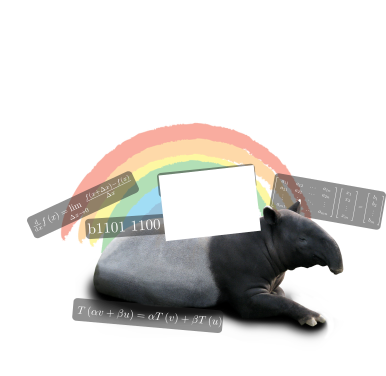
\includegraphics[width=5cm]{cover/tapir}};
				\node[rotate=-5, text=black!65] at (0.0,1.8) {$\langle \eb{i},\eb{j} \rangle = \delta_{ij}$};
				\node[rotate=5, text=black!45] at (-2.7,1.6) {$T\left( \alpha\vec{u} + \beta\vec{v} \right)=\alpha T\left( \vec{u} \right) + \beta T\left( \vec{v} \right)$};
				\node[rotate=-3, text=black!45] at (-0.5,2.7) {$A\vec{v}=\lambda\vec{v}$};
				\node[rotate=0, text=black!45] at (0.2,2.3) {$\int\limits_{a}^{b}f(x)\dif x = F(b)-F(a)$};
				\node[rotate=1, text=black!40] at (-3.0, 2.3) {$\Rot(\theta)=\begin{bmatrix}\cos(\theta) & -\sin(\theta) \\ \sin(\theta) & \cos(\theta) \end{bmatrix}$};
				\node[rotate=10, text=black!30] at (0.7,3.2) {$A=Q\Lambda Q^{-1}$};
				\node[rotate=-4, text=black!25] at (-0.8,3.4) {$\vec{v} = \sum\limits_{i=1}^{n}\alpha_{i}\eb{i}$};
				\node[rotate=0, text=black!20] at (0.9,3.8) {$\Rs{n}\overset{T}{\longrightarrow}\Rs{m}$};
				\node[rotate=0, text=black!20] at (-2.9,3.0) {$\od{f}{x}=\lim\limits_{\Delta x\rightarrow0}\frac{f(x+\Delta x)-f(x)}{\Delta x}$};
				\node[rotate=-3, text=black!10] at (-1.2,4.3) {$\int\limits_{a}^{b}f(x)\dif x = \lim\limits_{\Delta x\rightarrow0}\sum\limits_{k=1}^{N}f(x_{k})\Delta x$};
				\node[rotate=5, text=black!13] at (-2.5,3.7) {$\left( AB \right)^{\top} = B^{\top}A^{\top}$};
			\end{tikzpicture}
		}
	%\put(-10,85){%
	%
\includegraphics[width=6cm]{cover/gau_logo}
	%}
		\put(-10,-55){%
			\begin{minipage}[b][45mm][t]{226mm}
				\usebeamerfont{title}{\color{col2!20!black}\inserttitle\par}
				\color{col2!60!black}\rule{0.25\textwidth}{0.5pt}

				\vspace{3mm}
				\usebeamerfont{author}{\color{col2!40!black}\insertauthor}
			\end{minipage}
		}
  \end{picture}
}

\title{Basic Maths for Non-mathematicians}
\author{Peleg Bar Sapir}

%% ----- Document ----- %%

\begin{document}
\frame{\titlepage}

\ifdefined\full{
  \sectionpic{Introduction}{../figures/presentation_chapters/intro.pdf}

%% ----- Propositions ----- %%

\begin{frame}
  \frametitle{Mathematical Propositions}
  \begin{presentation_definition}
    A \emph{mathematical propostion} is a statement that can be either \true\ or \false.
  \end{presentation_definition}

  \onslide<2->{
    \begin{presentation_example}
      \begin{itemize}
          \onslide<2->{
          \item The Moon's radius is smaller than the Earth's radius (\true)
          }
          \onslide<3->{
          \item $1+2=3$ (\true)
          }
          \onslide<4->{
          \item Protons have no electric charge (\false)
          }
          \onslide<5->{
          \item $13 > 37$ (\false)
          }
      \end{itemize}
    \end{presentation_example}
  }
\end{frame}

\begin{frame}
  \frametitle{Operators: and, or}
  Propositions can be grouped together with \emph{operators} such as \textbf{and}, \textbf{or}.
  \begin{itemize}
      \onslide<2->{
      \item The \textbf{and} operator returns a \true\ statement only if \textbf{both} the statements it groups are themselves \true, otherwise it returns \false.
      }
      \onslide<3->{
      \item The \textbf{or} operator returns \true\ if \textbf{at least} one of the statements it groups is true.
      }
  \end{itemize}
\end{frame}

\begin{frame}
  \frametitle{Operators: and, or}
  \begin{presentation_example}
    \begin{align*}
      \onslide<1->{
        \thl{1+2=3} \text{ and } \thl{3-5=-2} &\Rightarrow \mtrue\\
      }
      \onslide<2->{
        \thl{1+2=3} \text{ and } \fhl{2\times4=7} &\Rightarrow \false\\
      }
      \onslide<3->{
        \fhl{\frac{10}{2}=1} \text{ and } \thl{2^{4}=16} &\Rightarrow \false\\
      }
      \onslide<4->{
        \fhl{7<5} \text{ and } \fhl{10+2=13} &\Rightarrow \false\\
      }
    \end{align*}
  \end{presentation_example}
\end{frame}

\begin{frame}
  \frametitle{Operators: and, or}
  \begin{presentation_example}
    \begin{align*}
      \onslide<1->{
        \thl{1+2=3} \text{ or } \fhl{3>7} &\Rightarrow \true\\
      }
      \onslide<2->{
        \fhl{0+3=-1} \text{ or } \thl{1=1} &\Rightarrow \true\\
      }
      \onslide<3->{
        \thl{2\times2=4} \text{ or } \thl{2+0=2} &\Rightarrow \true\\
      }
      \onslide<4->{
        \fhl{3\times7=10} \text{ or } \fhl{\frac{1}{2}<\frac{1}{10}} &\Rightarrow \false\\
      }
    \end{align*}
  \end{presentation_example}
\end{frame}

\begin{frame}
  \frametitle{Operators: Truth Table}
  We can summarize the behaviour of operators in a \emph{truth table}:
  \begin{table}
    \begin{tabular}[h]{p{1.5cm}p{1.5cm}p{1.5cm}p{1.5cm}}
      \toprule
      $A$ & $B$ & AND & OR\\
      \midrule
      \true & \true & \true & \true \\
      \true & \false & \false & \true \\
      \false & \true & \false & \true \\
      \false & \false & \false & \false \\
      \midrule
    \end{tabular}
  \end{table}
\end{frame}

\begin{frame}
  \frametitle{Mathematical Notation}
  Other \emph{notations} that will be used throughout this course:
  \begin{table}
    \begin{tabular}{ll}
      \toprule
      Symbol & In words\\
      \midrule
      $\neg a$ & \textbf{not} $a$\\
      $a \wedge b$ & $a$ \textbf{and} $b$\\
      $a \vee b$ & $a$ \textbf{or} $b$\\
      $a \Rightarrow b$ & $a$ \textbf{implies} $b$\\
      $a \Leftrightarrow b$ & $a$ \textbf{is equivalent to} $b$\\
      $\forall x$ & \textbf{For all} $x$ (...)\\
      $\exists x$ & \textbf{There exists} $x$ \textbf{such that} (...)\\
      $a\defeq b$ & $a$ \textbf{is defined to be} $b$\\
      \midrule
    \end{tabular}
  \end{table}
\end{frame}

%% ----- Sets ----- %%

\begin{frame}
  \frametitle{Sets}
  \onslide<1->{
    \begin{presentation_definition}
      A \emph{set} is a collection of \emph{elements}. Elements of a set can be any concept - be it physical (a chair, a car, a tapir) or abstract (a number, an idea).
    \end{presentation_definition}
  }

  \onslide<2->{
    \begin{presentation_note}
      In this course we consider only \emph{mathematical objects} as elements of sets.
    \end{presentation_note}
  }

  \onslide<3->{
    Sets can have a \emph{finite} or \emph{infinite} number of elements.
  }
\end{frame}

\begin{frame}
  \frametitle{Sets}
  \onslide<1->{
    Sets are denoted with curly brackets.
  }

  \onslide<2->{
    \begin{presentation_example}
      \begin{equation*}
        \left\{ 1,2,3,4 \right\},\quad\left\{ -4,\frac{3}{7},0,\pi,i,0.1 \right\},\quad\left\{ \text{all even numbers} \right\}.
      \end{equation*}
    \end{presentation_example}
  }
\end{frame}

\begin{frame}
  \frametitle{Sets}
  The order of elements in a set \textbf{does not matter}.

  \onslide<2->{
    \begin{presentation_example}
      The following sets are all identical:
      \begin{equation*}
        \left\{ 1,2,3,4 \right\} = \left\{ 1,3,2,4 \right\} = \left\{ 2,1,4,3 \right\}.
      \end{equation*}
    \end{presentation_example}
  }

  \onslide<3>{
    \begin{presentation_note}
      There is no repetition in sets, i.e. $\left\{ 1,1,3,3,3,3,5 \right\}$ is not a proper set, contrary to e.g. $\left\{ 1,3,5 \right\}$.
    \end{presentation_note}
  }
\end{frame}

\begin{frame}
  \frametitle{Sets}
  Sets can be denoted as conditions, using a vertical separator to denote \emph{conditions}.

  \onslide<2->{
    \begin{presentation_example}
      The following set contains all odd numbers between $0$ and $10$:
      \begin{equation*}
        \left\{ x \text{ is odd} \mid 0<x<10 \right\}.
      \end{equation*}

      \onslide<3>{
        It can also be written explicitly:
        \begin{equation*}
          \left\{ 1,3,5,7,9 \right\}.
        \end{equation*}
      }
    \end{presentation_example}
  }
\end{frame}

\begin{frame}
  \frametitle{Sets}
  Sets are usually denoted with an uppercase latin letter, while their elements as lowercase latin or greek letters. The notation $\in$ means that an element belongs to a set.
  \onslide<2>{
    \begin{presentation_example}
      For the two sets
      \begin{equation*}
        A = \left\{ 1,2,5,7 \right\},\quad B=\left\{ \text{even numbers} \right\},
      \end{equation*}
      all the following propostions are true:
      \begin{align*}
        &1\in A,\quad 2\in A,\quad 5\in A,\quad 7\in A,\\
        &2\in B,\quad 1\notin B,\quad 5\notin B,\quad 7\notin B.
      \end{align*}
    \end{presentation_example}
  }
\end{frame}

\begin{frame}
  \frametitle{Sets}
  The number of elements in a set (also called its \emph{cardinality}) is denoted with two vertical bars.

  \onslide<2>{
    \begin{presentation_example}
      \begin{equation*}
        S=\left\{ -3,0,-2,7,1 \right\}\quad\Rightarrow\quad|S|=5.
      \end{equation*}
    \end{presentation_example}
  }
\end{frame}

\begin{frame}
  \frametitle{The Empty Set}
  An important special set  is the \emph{empty set}, which is the set containing no elements. It is denoted by $\emptyset$, and has the unique property that
  \begin{equation*}
    \left| \emptyset \right| = 0.
  \end{equation*}
\end{frame}

\begin{frame}
  \frametitle{Subsets and Supersets}
  If a set $A$ contains all the elements in a set $B$ (and perhaps additional elements), then $B$ is said to be a \emph{subset} of $A$, and $A$ a \emph{superset} of $B$.

  \onslide<2>{
    \begin{presentation_example}
      The sets
      \begin{equation*}
        A=\left\{ 0,-3 \right\},\quad B=\left\{ 5,-3,1 \right\},\quad C=\left\{ -2,2,1 \right\},
      \end{equation*}
      are some of the subsets of
      \begin{equation*}
        D=\left\{ 0,-3,5,1,2,-2 \right\}.
      \end{equation*}
      Equivalently, $D$ is a superset of $A,B$ and $C$.
    \end{presentation_example}
  }
\end{frame}

\begin{frame}
  \frametitle{Subsets and Supersets}
  \begin{presentation_note}
    All sets are supersets and subsets of themselves. This is a direct consequence of the definition of supersets and subsets.
  \end{presentation_note}
\end{frame}

\begin{frame}
  \frametitle{Subsets and Supersets}
  We denote that $A$ is a superset of $B$ as
  \begin{equation*}
    B\subseteq A.
  \end{equation*}

  A \emph{Venn Diagram} representation of this fact looks as following:
  \begin{figure}[H]
    \centering
    \begin{tikzpicture}
      \def\firstcircle{(0,0) circle (2)}
      \def\secondcircle{(0.5,1) circle (0.75)}
      \begin{scope}
        \fill[col1!50]\firstcircle;
        \fill[col2!50]\secondcircle;
        \draw \firstcircle node[below] {$A$};
        \draw \secondcircle node [above] {$B$};
      \end{scope}
    \end{tikzpicture}
  \end{figure}
\end{frame}

\begin{frame}
  \frametitle{Subsets and Supersets}
  If for some two sets $A,B$ both $A\subseteq B$ \textbf{and} $B\subseteq A$, then the sets are identical.

  Formally, this fact is written as
  \begin{equation*}
    A\subseteq B \wedge B\subseteq A \Leftrightarrow A=B.
  \end{equation*}
\end{frame}

\begin{frame}
  \frametitle{Intersections and Unions}
  \begin{presentation_definition}
    The \emph{intersection} of two sets $A$ and $B$ is the set of all elements that are \textbf{both} in $A$ and in $B$.
  \end{presentation_definition}
  \onslide<2>{
    \begin{presentation_example}
      Given the sets
      \begin{equation*}
        A=\left\{ 1,2,5,6,7 \right\},\ B=\left\{ -1,0,1,5,10,13,15 \right\},
      \end{equation*}
      the intersection of $A$ and $B$ is $\left\{ 1, 5 \right\}$.
    }
  \end{presentation_example}
\end{frame}

\begin{frame}
  \frametitle{Intersections and Unions}
  The symbol denoting intersection is $\cap$. An intersection can be formally defined as
  \begin{equation*}
    A\cap B = \left\{ x \mid x\in A \wedge x\in B \right\}
  \end{equation*}
  (read: "the intersection of $A$ and $B$ is the set containing all elements $x$, such that $x$ is in $A$ and $x$ is in $B$")
\end{frame}

\begin{frame}
  \frametitle{Intersections and Unions}
  A Venn diagram visualization of $A\cap B$ (green area):
  \begin{figure}[H]
    \centering
    \begin{tikzpicture}
      \def\firstcircle{(0,0) circle (2)}
      \def\secondcircle{(2.3,0) circle (1.5)}
      \fill[col1!50]\firstcircle;
      \fill[col2!50]\secondcircle;
      \begin{scope}
        \clip \firstcircle;
        \fill[col3!50]\secondcircle;
      \end{scope}
      \draw\firstcircle node[left] {$A$};
      \draw\secondcircle node[right] {$B$};
      \draw (1.4,-0.2) node[above] {$A\cap B$};
    \end{tikzpicture}
  \end{figure}
\end{frame}

\begin{frame}
  \frametitle{Intersections and Unions}
  If the intersection of two sets is empty ($A\cap B=\emptyset$), then the sets are said to be \emph{disjoint}\index{Disjoint sets}:
  \begin{figure}[H]
    \centering
    \begin{tikzpicture}
      \def\firstcircle{(0,0) circle (2)}
      \def\secondcircle{(4,0) circle (1.5)}
      \fill[col1!50]\firstcircle;
      \fill[col2!50]\secondcircle;
      \draw\firstcircle node {$A$};
      \draw\secondcircle node {$B$};
    \end{tikzpicture}
  \end{figure}
\end{frame}

\begin{frame}
  \frametitle{Intersections and Unions}
  \begin{presentation_definition}
    The \emph{union}\index{Union of sets} of two sets $A,B$ is the set of all elements that are either in $A$ or in $B$ (or both).
  \end{presentation_definition}

  \onslide<2>{
    \begin{presentation_example}
      The union of the sets
      \begin{equation*}
        A=\left\{ -5, 7, 1\right\},\ B=\left\{ 10, -2, -5, 2 \right\},
      \end{equation*}
      is 
      \begin{equation*}
        A\cup B=\left\{ 10, -2, -5, 2, 7, 1 \right\}.
      \end{equation*}
    \end{presentation_example}
  }
\end{frame}

\begin{frame}
  \frametitle{Intersections and Unions}
  The symbol denoting union is $\cup$. A union can be formally defined as
  \begin{equation*}
    A\cup B = \left\{ x \mid x\in A \vee x\in B \right\}
  \end{equation*}
  (read: "the union of $A$ and $B$ is the set containing all elements $x$, such that $x$ is in $A$ or $x$ is in $B$")
\end{frame}

\begin{frame}
  \frametitle{Intersections and Unions}
  A Venn diagram visualization of $A\cup B$ (purple area):
  \begin{figure}[H]
    \centering
    \begin{tikzpicture}
      \def\firstcircle{(0,0) circle (2)}
      \def\secondcircle{(2.3,0) circle (1.5)}
      \fill[col4!50, draw=black]\firstcircle;
      \fill[col4!50, draw=black]\secondcircle;
      \draw\firstcircle node {$A$};
      \draw\secondcircle node {$B$};
    \end{tikzpicture}
  \end{figure}
\end{frame}

\begin{frame}
  \frametitle{Intersections and Unions}
  The number of elements in a union of two sets $A$ and $B$ is
  \begin{equation*}
    \left|A\cup B\right| = |A| + |B| - \left|A\cap B\right|
  \end{equation*}

  \onslide<2>{
    \begin{presentation_note}
      If $A,B$ are disjoint, $\left|A\cup B\right| = |A| + |B|$ (because $\left|A\cap B\right|=0$).
    \end{presentation_note}
  }
\end{frame}

\begin{frame}
  \frametitle{Difference of Sets}
  \begin{presentation_definition}
    The \emph{difference}\index{Difference of a set} of $A$ and $B$ is the set of all elements in $A$ that \emph{are not} elements of $B$. This is written as $A-B$ (or sometimes $A\setminus B$).
  \end{presentation_definition}
  \onslide<2>{
    \begin{presentation_example}
      For the sets
      \begin{equation*}
        A = \left\{ 1,5,9,10 \right\},\ B=\left\{ -3,2,5,9,13 \right\},
      \end{equation*}
      The differences are
      \begin{equation*}
        A-B=\left\{ 1,10 \right\},\ B-A=\left\{-3,2,13  \right\}.
      \end{equation*}
    \end{presentation_example}
  }
\end{frame}

\begin{frame}
  \frametitle{Difference of Sets}
  Formally:
  \begin{equation*}
    A-B = \left\{ x \mid x\in A,\ x\notin B\right\}
  \end{equation*}

  \onslide<2>{
    A Venn diagram visualization of $A-B$ (orange area):
    \begin{figure}[H]
      \centering
      \begin{tikzpicture}
        \def\firstcircle{(0,0) circle (2)}
        \def\secondcircle{(2.3,0) circle (1.5)}
        \begin{scope}
          \begin{scope}[even odd rule]% first circle without the second
            \clip \secondcircle (-3,-3) rectangle (3,3);
            \fill[col5!50] \firstcircle;
          \end{scope}
          \draw \firstcircle node {$A$};
          \draw \secondcircle node {$B$};
        \end{scope}
      \end{tikzpicture}
    \end{figure}
  }
\end{frame}

\begin{frame}
  \frametitle{Complement}
  \begin{presentation_definition}
    The \emph{complement}\index{Complement of a set} of a set $A$ in reltaion to a superset $Z\supset A$ is the difference $Z-A$, and is denoted $A^{\mathsf{c}}$.
  \end{presentation_definition}

  \onslide<2>{
    \begin{presentation_example}
      For the sets
      \begin{equation*}
        Z=\left\{ 1,2,3,4,5 \right\},\ A=\left\{ 1,2,3 \right\},
      \end{equation*}
      The complement of $A$ in relation to $Z$ is
      \begin{equation*}
        A^{\mathsf{c}}=\left\{ 4,5 \right\}
      \end{equation*}
    \end{presentation_example}
  }
\end{frame}

\begin{frame}
  \frametitle{Complement}
  Formally:
  \begin{equation*}
    A^{\mathsf{c}} = \left\{ x\in Z \mid x\notin A \right\}.
  \end{equation*}

  \onslide<2>{
    A Venn diagram representation:
    \begin{figure}[H]
      \centering
      \begin{tikzpicture}
        \def\firstcircle{(0,0) circle (2.5)}
        \def\secondcircle{(1,1) circle (1)}
        \fill[col1!50, draw=black]\firstcircle;
        \fill[col2!50, draw=black]\secondcircle;
        \node at (1.3,1) {$A$};
        \node at (-1,0) {$A^{\mathsf{c}}$};
        \node at (-2.7,1.9) {$Z$};
      \end{tikzpicture}
    \end{figure}
  }
\end{frame}

\begin{frame}
  \frametitle{Power Sets}
  \begin{presentation_definition}
    The set of all subsets of a given set $A$ is called the \emph{powerset of $A$}\index{Powerset}.
  \end{presentation_definition}
  \onslide<2>{
    \begin{presentation_example}
      All the subsets of $A=\left\{ 1,2,3 \right\}$ are:
      \begin{equation*}
        \emptyset, \left\{ 1 \right\}, \left\{ 2 \right\}, \left\{ 3 \right\}, \left\{ 1,2 \right\}, \left\{ 1,3 \right\}, \left\{ 2,3 \right\}, \left\{ 1,2,3 \right\}.
      \end{equation*}
      Thus, the power set of $A$ is
      \begin{equation*}
        P(A) = \left\{ \emptyset, \left\{ 1 \right\}, \left\{ 2 \right\}, \left\{ 3 \right\}, \left\{ 1,2 \right\}, \left\{ 1,3 \right\}, \left\{ 2,3 \right\}, \left\{ 1,2,3 \right\} \right\}.
      \end{equation*}
    \end{presentation_example}
  }
\end{frame}

\begin{frame}
  \frametitle{Power Sets}
  \begin{presentation_note}
    The empty set $\emptyset$ is a subset of all sets. Each set is also a subset of itself.
  \end{presentation_note}
\end{frame}

\begin{frame}
  \frametitle{Important Number Sets}
  Some important number sets, which will be used frequently in the course (all with infinite number of elements):
  \begin{itemize}
      \onslide<2->{
      \item \textbf{The natural numbers} (symbol: $\mathbb{N}$). These are the numbers $1,2,3,\dots$.
      }
      \onslide<3->{
      \item \textbf{The integers} (symbol: $\mathbb{Z}$). These are the "whole numbers" (i.e. not fractions). They include all the natural numbers together with their negatives (i.e. $-1,-2,-3,\dots$) and $0$.
      }
      \onslide<4->{
      \item \textbf{The rational} numbers (symbol: $\mathbb{Q}$). As their name suggests, they are ratios between two integers (e.g. $\frac{1}{2},\ \frac{-5}{3},\ \frac{7}{13}$).
      }
      \onslide<5->{
      \item \textbf{The real numbers} (symbol: $\mathbb{R}$). These are all the numbers on the number line (e.g. $2, \pi, \frac{\sqrt{3}}{17}, \sqrt{5}, -7.2, e^{\pi}$). A proper definition of the real numbers is beyond the scope of this course.
      }
  \end{itemize}
\end{frame}

\begin{frame}
  \frametitle{Important Number Sets}
  Additionaly, the \emph{Complex Numbers} are the set of all numbers
  \begin{equation*}
    z=a+bi,
  \end{equation*}
  where $a$ and $b$ are both real numbers, and $i$ is the imaginary unit, i.e. $i=\sqrt{-1}$.

  The complex number set has the notation $\mathbb{C}$.
\end{frame}

\begin{frame}
  \frametitle{Important Number Sets}
  Table summary:

  \begin{tabular}{lll}
    \toprule
    Symbol & Name & Definition \\
    \midrule
    $\mathbb{N}$ & Natural numbers & $\left\{1,2,3,4,\dots\right\}$\\
    $\mathbb{Z}$ & Integers & $\left\{ 0,\pm x \mid x\in\mathbb{N} \right\}$\\
    $\mathbb{Q}$ & Rational numbers & $\left\{ \frac{p}{q} \mid p\in\mathbb{Z}, q\in\mathbb{N} \right\}$\\
    $\mathbb{R}$ & Real numbers & Not in this course \\
    $\mathbb{C}$ & Complex numbers & $\left\{ a+ib \mid a,b\in\mathbb{R}, i=\sqrt{-1} \right\}$\\
    \midrule
  \end{tabular}
\end{frame}

\begin{frame}
  \frametitle{Important Number Sets}
  \begin{presentation_note}
    The relations between these sets are
    \begin{equation*}
      \mathbb{N}\subset \mathbb{Z}\subset\mathbb{Q}\subset\mathbb{R}\subset\mathbb{C}
    \end{equation*}
    (the symbol $\subset$ means "a proper subset")
  \end{presentation_note}
  \onslide<2>{
    \begin{presentation_note}
      Although each of these sets is infinite, the actual number of elements in $\mathbb{R}$ and $\mathbb{C}$ \textbf{is bigger} than the number of elements in $\mathbb{N},\mathbb{Z}$ and $\mathbb{Q}$. There are different kinds of infinities.
    \end{presentation_note}
  }
\end{frame}

\begin{frame}
  \frametitle{Intervals}
  The \emph{interval} $[a,b]$ is the subset of $\mathbb{R}$ defined as
  \begin{equation*}
    [a,b] = \left\{ x\in\mathbb{R} \mid a \leq x \leq b \right\}.
  \end{equation*}
  \begin{presentation_example}
    The interval $I=[-5,3]$ is the set of all real numbers that are \textbf{greater than or equal} to $-5$ and are \textbf{smaller than or equal} $3$.

    Some examples:
    \begin{equation*}
      -5.1 \notin I,\ -5 \in I,\ 0 \in I,\ 2 \in I,\ 3\in I,\ 4\notin I.
    \end{equation*}
  \end{presentation_example}
\end{frame}

\begin{frame}
  \frametitle{Intervals}
  The interval $(a,b)$ is the subset of $\mathbb{R}$ defined as
  \begin{equation*}
    [a,b] = \left\{ x\in\mathbb{R} \mid a < x < b \right\}.
  \end{equation*}
  (i.e. same as $[a,b]$ but excluding the actual values $a$ and $b$)
  \begin{presentation_example}
    The interval $I=(-5,3)$ is the set of all real numbers that are \textbf{greater than} $-5$ and are \textbf{smaller than} $3$.

    Some examples:
    \begin{equation*}
      -5.1\notin I,\ -5 \notin I,\ 0 \in I,\ 2 \in I,\ 3\notin I,\ 4\notin I.
    \end{equation*}
  \end{presentation_example}
\end{frame}

\begin{frame}
  \frametitle{Intervals}
  Similarily, the interval $[a,b)$ is the subset of $\mathbb{R}$ defined as
  \begin{equation*}
    [a,b) = \left\{ x\in\mathbb{R} \mid a \leq x < b \right\},
  \end{equation*}
  and the interval $(a,b]$ is the subset of $\mathbb{R}$ defined as
  \begin{equation*}
    (a,b] = \left\{ x\in\mathbb{R} \mid a < x \leq b \right\}.
  \end{equation*}
  (i.e. in the notation for intervals a square bracket means "less/more than or equal to", while a round braket means "less/more than" - without the "equal to" part)
\end{frame}

\begin{frame}
  \frametitle{Cartesian Products}
  \begin{presentation_definition}
    The \emph{cartesian product}\index{Cartesian product} of two sets $A,B$ (denoted $A\times B$) is the set of all possible \textbf{ordered} pairs, where the first component is an element of $A$ and the second component is an element of $B$.
  \end{presentation_definition}
  \onslide<2>{
    \begin{presentation_example}
      Consider $A=\left\{ 1,2,3 \right\},\ B=\left\{ x, y \right\}$. Then:
      \begin{equation*}
        A\times B = \left\{ \left( 1,x \right), \left( 1,y \right), \left( 2,x \right), \left( 2,y \right), \left( 3,x \right), \left( 3,y \right) \right\}
      \end{equation*}
    \end{presentation_example}
  }
\end{frame}

\begin{frame}
  \frametitle{Cartesian Products}
  \begin{presentation_note}
    The cartesian product of two sets $A,B$ is not commutative, i.e.
    \begin{equation*}
      A\times B \neq B\times A,
    \end{equation*}
    unless $A=B$ or any one of the sets (or both) is the empty set.
  \end{presentation_note}
\end{frame}

\begin{frame}
  \frametitle{Cartesian Products}
  Defining a cartesian product formally:
  \begin{equation*}
    A \times B = \left\{ (a,b) \mid a\in A,b\in B \right\}.
  \end{equation*}

  \onslide<2->{
    The number of elements in a cartesian product is
    \begin{equation*}
      \left|A\times B\right| = |A|\cdot|B|.
    \end{equation*}
  }

  \onslide<3>{
    The definition of a cartesian product can be expanded to $n\in\mathbb{N}$ sets $A_{1}, A_{2}, \dots, A_{n}$:
    \begin{equation*}
      A_{1}\times A_{2} \times \dots \times A_{n} = \left\{ \left(a_{1}, a_{2}, \dots, a_{n}\right) \mid a_{1}\in A_{1}, a_{2}\in A_{2}, \dots, a_{n}\in A_{n} \right\}
    \end{equation*}
  }
\end{frame}

\begin{frame}
  \frametitle{Cartesian Products}
  The definition can be made more compact by the use of the product symbol $\prod$:
  \begin{equation*}
    \prod\limits_{i=1}^{n} A_{i} = \left\{ \left( a_{1}, a_{2}, \dots, a_{i} \right) \mid a_{i}\in A_{i}, i=1,2,\dots,n\right\}.
  \end{equation*}

  \onslide<2>{
    \begin{presentation_note}
      The symbol $\prod$ is a generalized product notation. It will be discussed in more details later in the course.
    \end{presentation_note}
  }
\end{frame}

\begin{frame}
  \frametitle{Cartesian Products}
  A cartesian product of the same set is written in an similar way to a power. For example
  \begin{align*}
    \mathbb{R}\times\mathbb{R} &= \mathbb{R}^{2},\\
    \mathbb{R}\times\mathbb{R}\times\mathbb{R} &= \mathbb{R}^{3}.
  \end{align*}
  These are, respectively, sets of pairs of real numbers, e.g. $\left( -3,1 \right), (\pi,2), (-\frac{\sqrt{7}}{13}, 0)$, and triples of real numbers, e.g. $\left( 1,2,-\pi \right), \left( -6,\frac{1}{\sqrt{\pi}}, 0.2 \right), \left( \frac{1}{51}, \sqrt{3}, -4 \right)$.
\end{frame}

\begin{frame}
  \frametitle{Cartesian Products}
  \begin{presentation_example}
    For the set $A=\left\{ a,b \right\}$,
    \begin{equation*}
      A^{3}=\left\{(aaa),(aab),(aba),(abb),(baa),(bab),(bba),(bbb)\right\}.
    \end{equation*}

    \onslide<2>{
      For the set $B=\left\{ 1,2,3 \right\}$,
      \begin{align*}
        B^{2} = &\left\{(1,1),(1,2),(1,3),(2,1),(2,2),(2,3),\right.\\
        &\left.\ (3,1),(3,2),(3,3)\right\}.
      \end{align*}
    }
  \end{presentation_example}
\end{frame}

\begin{frame}
  \frametitle{Relations Between Sets}
  \begin{presentation_definition}
    A \emph{relation}\index{Relation between two sets} between two sets $A$ and $B$ is a way to "connect" the elements in the two sets in pairs. It is a subset of the cartesian product $A\times B$.
  \end{presentation_definition}

  \onslide<2>{
    \begin{presentation_example}
      An example relation between the sets $A=\left\{ 1,2,3,4,5 \right\}$ and $B=\left\{ \alpha,\beta,\gamma \right\}$ is
      \begin{equation*}
        R = \left\{(1,\alpha),(2,\alpha),(3,\beta),(3,\gamma),(5,\gamma)\right\}.
      \end{equation*}
    \end{presentation_example}
  }
\end{frame}

\tikzset{relation/.style={->, >=stealth, thick}}
\begin{frame}
  \frametitle{Relations Between Sets}
  The previous relation can be visually represented as following:
  \begin{figure}[H]
    \centering
    \begin{tikzpicture}[scale=0.8]
      \fill[col1!20, draw=col1, thick] (0,0) circle [x radius=0.75, y radius=2]; 
      \node (A1) at (0,1.5) {1};
      \node (A2) at (0,0.75) {2};
      \node (A3) at (0,0) {3};
      \node (A4) at (0,-0.75) {4};
      \node (A5) at (0,-1.5) {5};
      \node[above=5mm of A1] {\color{col1}$A$};

      \fill[col2!20, draw=col2, thick] (2,0) circle [x radius=0.75, y radius=1.5]; 
      \node (B1) at (2,1) {$\alpha$};
      \node (B2) at (2,0) {$\beta$};
      \node (B3) at (2,-1) {$\gamma$};
      \node[above=5mm of B1] {\color{col2}$B$};

      \draw[relation] (A1) -- (B1);
      \draw[relation] (A2) -- (B1);
      \draw[relation] (A3) -- (B2);
      \draw[relation] (A3) -- (B3);
      \draw[relation] (A5) -- (B3);
    \end{tikzpicture}
  \end{figure}

  \onslide<2>{
    \begin{presentation_note}
      Notice how not all elements are connected, and some elements in each set are connected to the same element in the other set. 
    \end{presentation_note}
  }
\end{frame}

\begin{frame}
  \frametitle{Reversed Relations}
  The previous relation can be reversed, yielding a subset of $B\times A$:
  \begin{equation*}
    R^{-1} = \left\{ (\alpha,1),(\alpha,2),(\beta,3),(\gamma,3),(\gamma,5) \right\}.
  \end{equation*}

  \onslide<2>{
    Graphically:
    \begin{figure}[H]
      \centering
      \begin{tikzpicture}[scale=0.8]
        \fill[col1!20, draw=col1, thick] (0,0) circle [x radius=0.75, y radius=2]; 
        \node (A1) at (0,1.5) {1};
        \node (A2) at (0,0.75) {2};
        \node (A3) at (0,0) {3};
        \node (A4) at (0,-0.75) {4};
        \node (A5) at (0,-1.5) {5};
        \node[above=5mm of A1] {\color{col1}$A$};

        \fill[col2!20, draw=col2, thick] (2,0) circle [x radius=0.75, y radius=1.5]; 
        \node (B1) at (2,1) {$\alpha$};
        \node (B2) at (2,0) {$\beta$};
        \node (B3) at (2,-1) {$\gamma$};
        \node[above=5mm of B1] {\color{col2}$B$};

        \draw[relation] (B1) -- (A1);
        \draw[relation] (B1) -- (A2);
        \draw[relation] (B2) -- (A3);
        \draw[relation] (B3) -- (A3);
        \draw[relation] (B3) -- (A5);
      \end{tikzpicture}
    \end{figure}
  }
\end{frame}

\begin{frame}
  \frametitle{Functions}
  \begin{presentation_definition}
    A \emph{function}\index{Function} between the sets $A,B$ is a relation in which for every element $a\in A$ there is exactly \textbf{one} connection to an element $b\in B$.
  \end{presentation_definition}

  \onslide<2>{
    \begin{presentation_example}
      A function from a set $A$ to a set $B$:
      \begin{figure}[H]
        \centering
        \begin{tikzpicture}[scale=0.6]
          \fill[col1!20, draw=col1, thick] (0,0) circle [x radius=0.75, y radius=2]; 
          \node (A1) at (0,1.5) {$1$};
          \node (A2) at (0,0.75) {$2$};
          \node (A3) at (0,0) {$3$};
          \node (A4) at (0,-0.75) {$4$};
          \node (A5) at (0,-1.5) {$5$};
          \node[above=5mm of A1] {\color{col1}$A$};

          \fill[col2!20, draw=col2, thick] (2,0) circle [x radius=0.75, y radius=1.75]; 
          \node (B1) at (2,1.2) {$\alpha$};
          \node (B2) at (2,0.4) {$\beta$};
          \node (B3) at (2,-0.4) {$\gamma$};
          \node (B4) at (2,-1.2) {$\delta$};
          \node[above=5mm of B1] {\color{col2}$B$};

          \draw[relation] (A1) -- (B1);
          \draw[relation] (A2) -- (B1);
          \draw[relation] (A3) -- (B2);
          \draw[relation] (A4) -- (B4);
          \draw[relation] (A5) -- (B3);
        \end{tikzpicture}
      \end{figure}

    \end{presentation_example}
  }
\end{frame}

\begin{frame}
  \frametitle{Functions}
  \begin{presentation_example}
    A relation which is \textbf{NOT} a function from $A$ to $B$:
    \begin{figure}[H]
      \centering
      \begin{tikzpicture}[scale=0.6]
        \fill[col1!20, draw=col1, thick] (0,0) circle [x radius=0.75, y radius=2]; 
        \node (A1) at (0,1.5) {$1$};
        \node (A2) at (0,0.75) {$2$};
        \node (A3) at (0,0) {$3$};
        \node (A4) at (0,-0.75) {$4$};
        \node (A5) at (0,-1.5) {$5$};
        \node[above=5mm of A1] {\color{col1}$A$};

        \fill[col2!20, draw=col2, thick] (2,0) circle [x radius=0.75, y radius=1.75]; 
        \node (B1) at (2,1.2) {$\alpha$};
        \node (B2) at (2,0.4) {$\beta$};
        \node (B3) at (2,-0.4) {$\gamma$};
        \node (B4) at (2,-1.2) {$\delta$};
        \node[above=5mm of B1] {\color{col2}$B$};

        \draw[relation] (A1) -- (B1);
        \draw[relation] (A2) -- (B1);
        \draw[relation] (A3) -- (B3);
        \draw[relation] (A4) -- (B4);
        \draw[relation, red] (A5) -- (B2.west);
        \draw[relation, red] (A5) -- (B4);
      \end{tikzpicture}
    \end{figure}
  \end{presentation_example}
\end{frame}

\begin{frame}
  \frametitle{Functions}
  Two additional terms that are used interchangeably with function are \emph{transformation} and \emph{map}. 
\end{frame}

\begin{frame}
  \frametitle{Functions}
  \begin{presentation_note}
    A function can have more than one element $a\in A$ connected to the same element $b\in B$. The only restriction is that no element $a\in A$ is connected to \textbf{more than one} element $b\in B$.
  \end{presentation_note}
\end{frame}

\tikzset{highlight/.style n args={1}{fill=col#1!20, draw=col#1, thick, rounded corners, minimum width=5mm, minimum height=5mm}}
\begin{frame}
  \frametitle{Functions}
  A common notation to a function $f$ connecting between elements of the sets $A$ and $B$ is
  \begin{equation*}
    \only<1>{
      f: \tikznode[highlight={1}, fill opacity=0, draw opacity=0, text opacity=1]{A}{A} \longrightarrow \tikznode[highlight={1}, fill opacity=0, draw opacity=0, text opacity=1]{B}{B}.
    }
    \only<2>{
      f: \tikznode[highlight={1}]{A}{A} \longrightarrow \tikznode[highlight={1}, fill opacity=0, draw opacity=0, text opacity=1]{B}{B}.
    }
    \only<3>{
      f: \tikznode[highlight={1}]{A}{A} \longrightarrow \tikznode[highlight={3}]{B}{B}.
    }
  \end{equation*}

  \begin{tikzpicture}[overlay, remember picture]
    \onslide<2->{
      \node[highlight={1}, below left=of A, xshift=1cm] (Atext) {Domain of $f$};
      \draw[vector, col1] (Atext.north) to [in=-90, out=90] (A.south);
    }
    \onslide<3>{
      \node[highlight={3}, below right=of B, xshift=-1cm] (Btext) {Image of $f$};
      \draw[vector, col3] (Btext.north) to [in=-90, out=90] (B.south);
    }
  \end{tikzpicture}
\end{frame}

\begin{frame}
  \frametitle{Functions}
  When used in practice, a common notation to show that an element $x\in A$ is connected to another element $y\in B$ is
  \begin{equation*}
    f(x) = y,
  \end{equation*}
  i.e. the function $f$ applied to the element $x\in A$ returns the element $y\in B$.
\end{frame}

\begin{frame}
  \frametitle{Real Functions}
  In part 3 of the course we will deal with functions of the form
  \begin{equation*}
    f:\mathbb{R} \longrightarrow \mathbb{R},
  \end{equation*}
  which we call \emph{real functions}, i.e. functions that take a real number $x$ and return a real number $y$.

  \onslide<2>{
    \begin{presentation_example}
      The functions
      \begin{equation*}
        f_{1}(x) = 2x^{2}-5,\quad f_{2}(x) = \sin\left( \frac{x}{3} \right),\quad f_{3}(x) = \frac{1}{\sqrt{2\pi}}e^{-\frac{x^{2}}{2}}
      \end{equation*}
      are all real functions.
    \end{presentation_example}
  }
\end{frame}

\begin{frame}
  \frametitle{Plotting Real Functions}
  \only<1>{
    We can plot a real function $f$ on a cartesian coordinate system by drawing a dot in each coordinate $(x,y)$, where $x$ is an element in the domain of $f$, and $y$ is its image (i.e. $f(x) = y$).
  }
  \only<2>{
    \begin{presentation_example}
      Plotting the function $f(x)=x^{2}-x-1.5$:
      \begin{figure}[H]
        \centering
        \begin{tikzpicture}
          \begin{axis}[
              width=0.75\textwidth,
              height=0.75\textwidth,
              xmin=-2, xmax=2,
              ymin=-2, ymax=2,
              scale=1.0, restrict y to domain=-2:2,
              axis line style={-stealth}
            ]
            \addplot[col1, thick, samples=500, smooth]
            plot (\x, { \x^2-\x-1.5} );
          \end{axis}
        \end{tikzpicture}
      \end{figure}
    \end{presentation_example}
  }
\end{frame}

\begin{frame}
  \frametitle{Injective, Surjective and Bijective Functions}
  A function is called \emph{injective} if each of the elements in its \textbf{image} is connected to by a single element in its \textbf{domain}.

  \onslide<2>{
    \begin{presentation_example}  
      \begin{figure}[H]
        \centering
        \begin{tikzpicture}[scale=0.9]
  % Injective function
          \fill[col1!20, draw=col1, thick] (0,0) circle [x radius=0.75, y radius=2]; 
          \node (A1) at (0,1.5) {$1$};
          \node (A2) at (0,0.5) {$2$};
          \node (A3) at (0,-0.5) {$3$};
          \node (A4) at (0,-1.5) {$4$};
          \node[above=5mm of A1] {\color{col1}$A$};

          \fill[col2!20, draw=col2, thick] (2,0) circle [x radius=0.75, y radius=1.75]; 
          \node (B1) at (2,1.2) {$\alpha$};
          \node (B2) at (2,0.4) {$\beta$};
          \node (B3) at (2,-0.4) {$\gamma$};
          \node (B4) at (2,-1.2) {$\delta$};
          \node[above=5mm of B1] {\color{col2}$B$};

          \draw[relation] (A1) -- (B2);
          \draw[relation] (A2) -- (B3);
          \draw[relation] (A3) -- (B1);
          \draw[relation] (A4) -- (B4);

          \node at (1,3.5) {\underline{Injective}};

  % Non injective function
          \fill[col1!20, draw=col1, thick] (6,0) circle [x radius=0.75, y radius=2]; 
          \node (A1b) at (6,1.5) {$1$};
          \node (A2b) at (6,0.75) {$2$};
          \node (A3b) at (6,0) {$3$};
          \node (A4b) at (6,-0.75) {$4$};
          \node (A5b) at (6,-1.5) {$5$};
          \node[above=5mm of A1b] {\color{col1}$A$};

          \fill[col2!20, draw=col2, thick] (8,0) circle [x radius=0.75, y radius=1.75]; 
          \node (B1b) at (8,1.2) {$\alpha$};
          \node (B2b) at (8,0.4) {$\beta$};
          \node (B3b) at (8,-0.4) {$\gamma$};
          \node (B4b) at (8,-1.2) {$\delta$};
          \node[above=5mm of B1b] {\color{col2}$B$};

          \draw[relation] (A1b) -- (B1b);
          \draw[relation, red] (A2b) -- (B2b);
          \draw[relation, red] (A3b) -- (B2b);
          \draw[relation] (A4b) -- (B3b);
          \draw[relation] (A5b) -- (B4b);

          \node at (7,3.5) {\underline{Not injective}};
        \end{tikzpicture}
      \end{figure}
    \end{presentation_example}
  }
\end{frame}

\begin{frame}
  \frametitle{Injective, Surjective and Bijective Functions}
  A function is called \emph{surjective} if all of the elements in its \textbf{image} are connected to by some element in its \textbf{domain}.

  \onslide<2>{
    \begin{presentation_example}  
      \begin{figure}[H]
        \centering
        \begin{tikzpicture}[scale=0.9]
  % Surjective function
          \fill[col1!20, draw=col1, thick] (0,0) circle [x radius=0.75, y radius=2]; 
          \node (A1) at (0,1.5) {$1$};
          \node (A2) at (0,0.5) {$2$};
          \node (A3) at (0,-0.5) {$3$};
          \node (A4) at (0,-1.5) {$4$};
          \node[above=5mm of A1] {\color{col1}$A$};

          \fill[col2!20, draw=col2, thick] (2,0) circle [x radius=0.75, y radius=1.75]; 
          \node (B1) at (2,1.2) {$\alpha$};
          \node (B2) at (2,0.4) {$\beta$};
          \node (B3) at (2,-0.4) {$\gamma$};
          \node (B4) at (2,-1.2) {$\delta$};
          \node[above=5mm of B1] {\color{col2}$B$};

          \draw[relation] (A1) -- (B2);
          \draw[relation] (A2) -- (B3);
          \draw[relation] (A3) -- (B1);
          \draw[relation] (A4) -- (B4);

          \node at (1,3.5) {\underline{Surjective}};

  % Non surjective function
          \fill[col1!20, draw=col1, thick] (6,0) circle [x radius=0.75, y radius=2]; 
          \node (A1b) at (6,1.5) {$1$};
          \node (A2b) at (6,0.5) {$2$};
          \node (A3b) at (6,-0.5) {$3$};
          \node (A4b) at (6,-1.5) {$4$};
          \node[above=5mm of A1b] {\color{col1}$A$};

          \fill[col2!20, draw=col2, thick] (8,0) circle [x radius=0.75, y radius=1.75]; 
          \node (B1b) at (8,1.2) {$\alpha$};
          \node (B2b) at (8,0.4) {$\beta$};
          \node (B3b) at (8,-0.4) {$\gamma$};
          \node[text=red] (B4b) at (8,-1.2) {$\delta$};
          \node[above=5mm of B1b] {\color{col2}$B$};

          \draw[relation] (A1b) -- (B1b);
          \draw[relation] (A2b) -- (B2b);
          \draw[relation] (A3b) -- (B3b);
          \draw[relation] (A4b) -- (B3b);

          \node at (7,3.5) {\underline{Not surjective}};
        \end{tikzpicture}
      \end{figure}
    \end{presentation_example}
  }
\end{frame}

\begin{frame}
  \frametitle{Injective, Surjective and Bijective Functions}
  A function that is both \textbf{injective} and \textbf{surjective} is called \emph{bijective}.
\end{frame}

\begin{frame}
  \frametitle{Injective, Surjective and Bijective Functions}
  \begin{presentation_example}
    Let's look at a few examples of real injective, surjective and bijective functions over $\mathbb{R}$:
    \begin{itemize}
      \item
        \only<1>{$f(x)=x$, injective + surjective = bijective.}
        \only<2>{$f(x)=x^{2}$, neither injective nor surjective.}
        \only<3>{$f(x)=x^{3}-2x^{2}$, surjective.}
        \only<4>{$f(x)=e^{x}$, injective.}
        \only<5>{$f(x)=\sin(x)$, neither injective nor surjective.}
        \begin{figure}[H]
          \centering
          \begin{tikzpicture}[scale=0.75]
            \tikzset{function/.style={ultra thick, samples=100}}
            \begin{axis}[
                domain=-4.5:4.5,
                xmin=-4.5, xmax=4.5,
                ymin=-4.5, ymax=4.5,
                every axis x label/.style={
                  at={(ticklabel* cs:1.03)},
                  anchor=west,
                },
                every axis y label/.style={
                  at={(ticklabel* cs:1.03)},
                  anchor=south,
                },
              axis line style={-stealth},]
              \only<1>{\addplot[function, col1] {x};}
              \only<2>{\addplot[function, col2] {x^2};}
              \only<3>{\addplot[function, col3] {x^3-2*x^2};}
              \only<4>{\addplot[function, col4] {exp(x)};}
              \only<5>{\addplot[function, col5] {sin(deg(x))};}
            \end{axis}
          \end{tikzpicture}
        \end{figure}
    \end{itemize}
  \end{presentation_example}
\end{frame}

\begin{frame}
  \frametitle{Injective, Surjective and Bijective Functions}
  \begin{presentation_note}
    Every non-surjective function can be made surjective by excluding the elements its image that are not connected to by any element in its domain.\\

    For example, the function $f(x)=\sin(x)$ is not surjective as a function $\func{f}{\mathbb{R}}{\mathbb{R}}$, but is surjective as a function $\func{f}{\mathbb{R}}{[-1,1]}$.
  \end{presentation_note}
\end{frame}

\begin{frame}
  \frametitle{Multivariable Functions}
  Functions may have several arguments and return several arguments.
  \onslide<2->{
    \begin{presentation_example}
      The following functions take as input three real numbers, and return a single real number ($f:\mathbb{R}^{3}\to\mathbb{R}$). The return value of some functions for a triplet of real numbers, $\left( -5,7,1 \right)$, are:
      \begin{itemize}
        \item $f\left( x,y,z \right)=x+y+z\Rightarrow f\left( -5,7,1 \right)=-5+7+1=3$
          \onslide<3->{
          \item $f\left( x,y,z \right)=x^{2}-y^{2}\Rightarrow f\left( -5,7,1 \right)=25-49=-24$
          }
          \onslide<4->{
          \item $f\left( x,y,z \right)=\frac{x}{\sqrt{y}+z}\Rightarrow f\left(-5,7,1  \right)=\frac{5}{\sqrt{7}+1}$
          }
      \end{itemize}
    \end{presentation_example}
  }
\end{frame}

\begin{frame}
  \frametitle{Multivariable Functions}
  \begin{presentation_example}
    The function $f:\mathbb{Z}\times\mathbb{N} \longrightarrow \mathbb{Q}$ is defined as
    \begin{equation*}
      f(p,q) = \frac{p}{q}.
    \end{equation*}
    The return values of $f$ for some example inputs are
    \begin{itemize}
        \onslide<2->{
        \item $f(1,2) = \frac{1}{2}$,
        }
        \onslide<3->{
        \item $f(-5,2) = -\frac{5}{2} = -2.5$,
        }
        \onslide<4>{
        \item $f(0,13) = \frac{0}{13} = 0$.
        }
    \end{itemize}
  \end{presentation_example}
\end{frame}

\begin{frame}
  \frametitle{Composition of Functions}
  Functions can be \emph{composed} together, generating new functions.
  \onslide<2->{
    \begin{presentation_example}
      Consider the functions
      \begin{equation*}
        f(x)=x^{2},\quad g(x)=\sin(x).
      \end{equation*}
      We can compose the two functions in two ways:
      \begin{itemize}
          \onslide<3-> \item $g_{1}(x) = f\left( g(x) \right) = \left[\sin(x)\right]^{2}$, and
          \onslide<4-> \item $g_{2}(x) = g\left( f(x) \right) = \sin(x^{2})$.
      \end{itemize}
    \end{presentation_example}
  }
\end{frame}

\begin{frame}
  \frametitle{Composition of Functions}
  We denote a composition of two functions $\func{f}{A}{B}$ and $\func{g}{B}{C}$ as
  \begin{equation*}
    \func{g \circ f}{A}{C}.
  \end{equation*}
  \begin{presentation_note}
    For a composition to be valid, the \textbf{domain} of the second function (here $g$) must be the same as the \textbf{image} of the first function.
  \end{presentation_note}
\end{frame}

\begin{frame}
  \frametitle{Composition of Functions}
  \begin{presentation_example}
    A graphical representation of composing two functions:
    \begin{figure}[H]
      \centering
      \begin{tikzpicture}[scale=0.9]
        \fill[col1!20, draw=col1, thick] (0,0) circle [x radius=0.75, y radius=2]; 
        \node (A1) at (0,1.5) {$1$};
        \node (A2) at (0,0.5) {$2$};
        \node (A3) at (0,-0.5) {$3$};
        \node (A4) at (0,-1.5) {$4$};
        \node[above=5mm of A1] {\color{col1}$A$};

        \onslide<1>{
          \fill[col2!20, draw=col2, thick] (3,0) circle [x radius=0.75, y radius=1.75]; 
          \node (B1) at (3,1.2) {$\alpha$};
          \node (B2) at (3,0.4) {$\beta$};
          \node (B3) at (3,-0.4) {$\gamma$};
          \node (B4) at (3,-1.2) {$\delta$};
          \node[above=5mm of B1] {\color{col2}$B$};

          \draw[relation, thick] (1,2) -- node [midway, above] {$f$} ++(1,0);
          \draw[relation, thick] (4,2) -- node [midway, above] {$g$} ++(1,0);
        }

        \fill[col3!20, draw=col3, thick] (6,0) circle [x radius=0.75, y radius=1.5]; 
        \node (C1) at (6,1) {$a$};
        \node (C2) at (6,0) {$b$};
        \node (C3) at (6,-1) {$c$};
        \node[above=5mm of C1] {\color{col3}$C$};

        \onslide<1>{
          \draw[relation] (A1) -- (B2);
          \draw[relation] (A2) -- (B4);
          \draw[relation] (A3) -- (B1);
          \draw[relation] (A4) -- (B3);
          \draw[relation] (B1) -- (C2);
          \draw[relation] (B2) -- (C3);
          \draw[relation] (B3) -- (C1);
          \draw[relation] (B4) -- (C3);
        }
        \onslide<2>{
          \draw[relation] (A1) -- (C3);
          \draw[relation] (A2) -- (C3);
          \draw[relation] (A3) -- (C2);
          \draw[relation] (A4) -- (C1);
          \draw[relation, thick] (1,2) -- node [midway, above] {$g\circ f$} ++(4,0);
        }
      \end{tikzpicture}
    \end{figure}
  \end{presentation_example}
\end{frame}

% -- Some definitions for graphs
\tikzset{
  between/.style args={#1 and #2}{
    at = ($(#1)!0.5!(#2)$)
  }
}

\begin{frame}
  \frametitle{Graphs}
  \begin{presentation_definition}
    A \emph{graph} is a mathematical structure composed of \emph{nodes} connected to other nodes by \emph{edges}.
  \end{presentation_definition}

  \onslide<2>{
    \begin{presentation_example}
      A graph with 5 nodes and 7 edges:
      \begin{figure}[H]
        \centering
        \begin{tikzpicture}
          \tikzset{every state/.style={graphstate, fill=col1}}
          \node[state] (A) {};
          \node[state] (B) [right=of A] {};
          \node[state] (C) [below=of A] {};
          \node[state] (D) [below=of B] {};
          \node[state] (E) [between=B and D, xshift=2cm] {};

          \path (A) edge node {} (B)
          (B) edge node {} (D)
          (C) edge node {} (A)
          (D) edge node {} (C)
          (E) edge node {} (B)
          (E) edge node {} (D)
          (A) edge node {} (D);

          \node[col1, left=of A] (nodetxt) {\textbf{Node}};
          \node[above left=of C, yshift=-4mm] (edgetxt) {\textbf{Edge}};
          \node[between=A and C] (edge) {};

          \draw[vector, densely dotted, col1] (nodetxt.east) to ($(A.west)+(-1mm,0)$);
          \draw[vector, densely dotted] (edgetxt.east) to (edge);
        \end{tikzpicture}
      \end{figure}
    \end{presentation_example}
  }
\end{frame}

\begin{frame}
  \frametitle{Graphs}
  In the graphical representation of a graph, the actual position of nodes does not matter - what matters are the connections (edges) between them.

  \onslide<2>{
    \begin{presentation_example}
      The following three graphs are identical:
      \begin{figure}[H]
        \centering
        \begin{tikzpicture}[-, >=stealth, auto, semithick]
          \tikzset{every state/.style={graphstate, fill=col2!75}}

  % First representation
          \node[state] (A1)  {};
          \node[state] (B1) [right=of A1]  {};
          \node (AB1) [between=A1 and B1]  {};
          \node[state] (C1) [below=of AB1] {};

          \path (A1) edge node {} (B1)
          (B1) edge node {} (C1)
          (C1) edge node {} (A1);

  % Second representation
          \node[state] (A2) [right=3cm of A1] {};
          \node[state] (B2) [below=of A2] {};
          \node[state] (C2) [below left=of B2, yshift=5mm]{};

          \path (A2) edge node {} (B2)
          (B2) edge node {} (C2)
          (C2) edge node {} (A2);

  % Third representation
          \node[state] (A3) [right=1cm of A2] {};
          \node[state] (B3) [below=of A3] {};
          \node[state] (C3) [right=of B3] {};

          \path (A3) edge node {} (B3)
          (B3) edge node {} (C3)
          (C3) edge [bend right] node {} (A3);
        \end{tikzpicture}
      \end{figure}
    \end{presentation_example}
  }
\end{frame}

\begin{frame}
  \frametitle{Graphs}
  \begin{presentation_definition}
    A graph in which edges have directions is called a \emph{directed graph}.
  \end{presentation_definition}

  \onslide<2>{
    \begin{presentation_example}
      A directed graph with 4 nodes and 6 edges:
      \begin{figure}[H]
        \centering
        \begin{tikzpicture}[->, >=stealth', auto, semithick]
          \tikzset{every state/.style={graphstate, fill=col3!75}}

          \node[state] (A) {};
          \node[state] (C) [below=of A] {};
          \node (AC) [between=A and C] {};
          \node[state] (B) [left=of AC] {};
          \node[state] (D) [right=of AC] {};

          \path (A) edge [bend left] node {} (B);
          \path (B) edge [bend left] node {} (A);
          \path (B) edge node {} (C);
          \path (C) edge node {} (D);
          \path (D) edge node {} (A);
          \path (D) edge [loop right] node {} (D);
        \end{tikzpicture}
      \end{figure}
    \end{presentation_example}
  }
\end{frame}

\begin{frame}
  \frametitle{Graphs}
  \begin{presentation_definition}
    A \emph{path} in a graph is a sequence of edges in which each edge shares a vertex with the previous edge (except the first edge).
  \end{presentation_definition}
  \onslide<2>{
    \begin{presentation_example}
      A path in a graph (note that the nodes are labeled):
      \begin{figure}[H]
        \centering
        \begin{tikzpicture}
          \tikzset{every state/.style={graphstate, fill=col4!50}}

          \node[state] (1) {1};
          \node[state, below=of 1] (2) {2};
          \node[state, right=of 2] (3) {3};
          \node[state, above=of 3] (4) {4};
          \node[state, right=of 4] (5) {5};
          \node[state, below=of 5] (6) {6};
          \node[state, right=of 6] (7) {7};
          \node[state, above=of 7] (8) {8};

          \path (1) edge [ultra thick, red] node {} (2);
          \path (1) edge node {} (3);
          \path (1) edge node {} (4);
          \path (2) edge [ultra thick, red] node {} (3);
          \path (3) edge node {} (4);
          \path (3) edge [ultra thick, red] node {} (5);
          \path (3) edge node {} (6);
          \path (4) edge node {} (5);
          \path (5) edge [ultra thick, red] node {} (6);
          \path (5) edge node {} (8);
          \path (5) edge node {} (7);
          \path (6) edge [ultra thick, red] node {} (7);
          \path (7) edge [ultra thick, red] node {} (8);
        \end{tikzpicture}
      \end{figure}
    \end{presentation_example}
  }
\end{frame}

\begin{frame}
  \frametitle{Graphs}
  \begin{presentation_definition}
    When the start and end vertices coincide the path is known as a \emph{circle}. A directed circle is known as a \emph{cycle}.
  \end{presentation_definition}
\end{frame}

\begin{frame}
  \frametitle{Graphs}
  \only<1>{
    \begin{presentation_definition}
      If one or more pathes exist between two vertices $a,b$ in a graph, the number of edges in the shortest path is defined to be the \emph{distance} between the two vertices, and is denoted as $\dist(a,b)$.
    \end{presentation_definition}
  }

  \only<2>{
    \begin{presentation_example}
      In the following graph three paths between vertices $a$ and $b$ are shown. The number of edges in the shortest path, highlighted in red, is defined as the distance $\dist(a,b)$, and is equal to 3.
      \begin{figure}[H]
        \centering
        \begin{tikzpicture}
          \tikzset{every state/.style={graphstate, fill=col2!75}}

          \node[state] (1) {a};
          \node[state, right=of 1] (a) { };
          \node[state, right=of a] (b) { };
          \node[state, right=of b] (2) {b};

          \path (1) edge [ultra thick, red] (a);
          \path (a) edge [ultra thick, red] (b);
          \path (b) edge [ultra thick, red] (2);

          \node[state, above right=of 1, xshift=-5mm] (c) { };
          \node[state, right=of c] (d) { };
          \node[state, right=of d] (e) { };

          \path (1) edge (c);
          \path (c) edge (d);
          \path (d) edge (e);
          \path (e) edge (2);

          \node[state, below right=of 1, xshift=-5mm] (f) { };
          \node[state, right=of f] (g) { };
          \node[state, right=of g] (h) { };

          \path (1) edge (f);
          \path (f) edge (g);
          \path (g) edge (h);
          \path (h) edge (2);
        \end{tikzpicture}
      \end{figure}
    \end{presentation_example}
  }
\end{frame}

\begin{frame}
  \frametitle{Graphs}
  \begin{presentation_definition}
    A \emph{tree} is a graph with no circles.
  \end{presentation_definition}
  \onslide<2>{
    \begin{presentation_example}
      A tree (notice that no circles are present):
      \begin{figure}[H]
        \centering
        \begin{tikzpicture}
          \tikzset{every state/.style={graphstate, minimum size=5mm, fill=col3!75}}
          \tikzset{node distance=5mm}

          \node[state] (1) { };
          \node[state, above left=of 1] (2) { };
          \node[state, above right=of 1] (3) { };
          \node[state, below=of 1] (4) { };
          \node[state, below left=of 4] (5) { };
          \node[state, below right=of 4] (6) { };
          \node[state, below=of 4] (7) { };
          \node[state, left=of 2] (8) { };
          \node[state, above right=of 3] (9) { };
          \node[state, below right=of 3] (10) { };

          \path (1) edge [ultra thick] (2);
          \path (1) edge [ultra thick] (3);
          \path (1) edge [ultra thick] (4);
          \path (4) edge [ultra thick] (5);
          \path (4) edge [ultra thick] (6);
          \path (4) edge [ultra thick] (7);
          \path (2) edge [ultra thick] (8);
          \path (3) edge [ultra thick] (9);
          \path (3) edge [ultra thick] (10);
        \end{tikzpicture}
      \end{figure}
    \end{presentation_example}
  }
\end{frame}

\begin{frame}
  \frametitle{Graphs}
  Some trees have a distinctive \emph{root} node, and are known as \emph{rooted trees}. A node that is "branched" from a higher level node is called a \emph{child node}. The last level nodes are called \emph{leaves} (singular: leaf). The rest of the nodes are known as \emph{inner nodes}.
\end{frame}

\begin{frame}
  \frametitle{Graphs}
  \begin{presentation_example}
    A rooted tree, with the root node highlighted in red and the leaves in green:
    \begin{figure}[H]
      \centering
      \begin{tikzpicture}[-, very thick]
        \tikzset{level/.style={sibling distance=4.2cm/####1, level distance=1.2cm}}
        \node [rnode] (root) { }
        child{ node (child1) [tnode] { }
          child{ node [tnode](child3) { }
            child{ node [lnode] (leaf1){ } edge from parent node[above left] {}}
          }
          child{ node [tnode] { }
            child{ node [lnode] (leaf2){ }}
            child{ node [lnode] (leaf3){}}
          }
        }
        child{ node [tnode](child2)  { }
          child{ node [tnode] { }
            child{ node [lnode] (leaf4) {}}
          }
          child{ node [tnode] { }
            child{ node [lnode] (leaf5){ }}
            child{ node [lnode] (leaf6){}}
            child{ node [lnode] (leaf7) {}}
          }
        }
        ;

        \node[annotationtext, right=of root] (roottxt) {Root};
        \draw[arr, annotation] (roottxt) to ($(root.east) + (2mm,0mm)$);

        \node[annotationtext, below=of root] (childtext) {Children of root};
        \draw[arr, annotation] (childtext) to ($(child1.east) + (2mm,0)$);
        \draw[arr, annotation] (childtext) to ($(child2.west) + (-2mm,0)$);

        \node[annotationtext, right=of child1.north] (br1) {};
        \node[annotationtext, right=of child3.south] (br2) {};
        \coordinate (A) at (-4.2,0);
        \draw[annotation, decorate, decoration={brace, amplitude=3pt, raise=-10pt, mirror}]
        (A |- br1) -- (A |- br2) node[annotationtext, midway, xshift=-1pt, rotate=90] {Inner nodes};

        \node[annotationtext, below = of root, yshift=-3.5cm] (leaves) {Leaves};
        \draw[annotation, arr] (leaves) -- ($(leaf1.south) + (0,-2mm)$);
        \draw[annotation, arr] (leaves) -- ($(leaf2.south) + (0,-2mm)$);
        \draw[annotation, arr] (leaves) -- ($(leaf3.south) + (0,-2mm)$);
        \draw[annotation, arr] (leaves) -- ($(leaf4.south) + (0,-2mm)$);
        \draw[annotation, arr] (leaves) -- ($(leaf5.south) + (0,-2mm)$);
        \draw[annotation, arr] (leaves) -- ($(leaf6.south) + (0,-2mm)$);
        \draw[annotation, arr] (leaves) -- ($(leaf7.south) + (0,-2mm)$);
      \end{tikzpicture}
    \end{figure}
  \end{presentation_example}
\end{frame}

\begin{frame}
  \frametitle{Graphs}
  \begin{presentation_definition}
    A tree with 2 children per node (except the leaves) is called a \emph{binary tree}. Similarily, trees can be ternary, quaternary, etc.
  \end{presentation_definition}
  \begin{presentation_example}
    A binary tree:
    \begin{figure}[H]
      \centering
      \begin{tikzpicture}[-, very thick]
        \tikzset{level/.style={sibling distance=3.5cm/####1, level distance=0.75cm}}
        \tikzset{tnode/.style = {treenode, circle, font=\sffamily\bfseries, draw=black,
        fill=col2!50, minimum size=4mm}}
        \node [tnode] (root) { }
        child{ node  [tnode] { }
          child{ node [tnode] { }
            child{ node [tnode] { }}
            child{ node [tnode] { }}
          }
          child{ node [tnode] { }
            child{ node [tnode] { }}
            child{ node [tnode] {}}
          }
        }
        child{ node [tnode]  { }
          child{ node [tnode] { }
            child{ node [tnode] { }}
            child{ node [tnode] { }}
          }
          child{ node [tnode] { }
            child{ node [tnode] { }}
            child{ node [tnode] {}}
          }
        };
      \end{tikzpicture}
    \end{figure}
  \end{presentation_example}
\end{frame}

\begin{frame}
  \frametitle{Graphs}
  Rooted trees are used to describe hierarchies, e.g. in biological systematics, organisations or nested directories of data.
\end{frame}

\begin{frame}
  \frametitle{Graphs}
  \begin{presentation_definition}
    The \emph{complete graph} $K_{n}$ is the graph with $n$ vertices where every pair of different vertices is connected by an edge (Also called a \emph{clique}).
  \end{presentation_definition}

  \onslide<2>{
    \begin{presentation_example}
      The cliques $K_{1}, \dots, K_{6}$:
      \newcommand{\clique}[3]{
        \pgfmathsetmacro{\ang}{180-((####1-2)*180/####1)}
        \pgfmathsetmacro{\anull}{90}
        \pgfmathsetmacro{\xnull}{####3}

        \foreach \n in {1,...,####1}{
          \node[state, fill=col####1!75] (p\n) at ({####2*cos(\n*\ang+\anull)+\xnull},{####2*sin(\n*\ang+\anull)}) { };
          \foreach \m in {1,...,\n}{
            \path (p\n) edge (p\m);
          }
        }

        \node at (\xnull,-1.5cm) {$K_{####1}$};
      }

      \begin{figure}[H]
        \centering
        \begin{tikzpicture}[node distance=1cm]
          \tikzset{every state/.style={graphstate, minimum size=2.5mm, fill=col2}}
          \foreach \K in {1,...,6}{
            \clique{\K}{0.5}{\K*1.75}
          }
        \end{tikzpicture}
      \end{figure}
    \end{presentation_example}
  }
\end{frame}

  \sectionpic{Vectors}{../figures/presentation_chapters/vectors.pdf}

\begin{frame}
  \frametitle{Basics of Vectors}
  There are 3 distinct approaches to describe what a vector is:
  \begin{itemize}
  \item The physicist's approach (geometric)
  \item The computer scientist's approach (algebraic)
  \item The mathematician's approach (abstract)
  \end{itemize}
\end{frame}

\begin{frame}
  \frametitle{Geometric Vectors}
  \begin{presentation_definition}
  A vector is an object with a length and a direction.
  \end{presentation_definition}

  \begin{figure}[H]
  \centering
  \begin{tikzpicture}[scale=0.75, align=center]
  \Large
  \draw[vector, col1] (0,0) -- (2,3);
  \draw[vector, col2] (-1,0) -- (-2,2);
  \draw[vector, col3] (0,-1) -- (-3,-1);
  \draw[vector, col4] (2,0) -- (1,-3);
  \draw[vector, col5] (-4,2) -- (-4,-2);
  \draw[vector, black] (-7,1) -- (-6,0);
  \end{tikzpicture}
  \end{figure}
\end{frame}

\begin{frame}
  \frametitle{Vector Notation}
  Vectors are denoted as latin letters with an arrow above them:
  \begin{equation*}
  \vec{u},\quad\vec{v},\quad\vec{x},\quad\vec{a},\quad\cdots
  \end{equation*}

  In maths and physics the following notations are mostly used:
  \begin{align*}
  \bm{u},\quad\bm{v},\quad\bm{x},\quad\bm{a},\quad\cdots\\
  \underline{\bm{u}},\quad\underline{\bm{v}},\quad\underline{\bm{x}},\quad\underline{\bm{a}},\quad\cdots\\
  \end{align*}
\end{frame}

\begin{frame}
  \frametitle{Geometric Vectors}
  We consider all vectors starting at the same point, called the \emph{origin}.

  \begin{figure}[H]
  \centering
  \begin{tikzpicture}[scale=0.75, align=center]
  \draw[vector, col1] (0,0) -- (2,3);
  \draw[vector, col2] (0,0) -- (-1,2);
  \draw[vector, col3] (0,0) -- (-3,0);
  \draw[vector, col4] (0,0) -- (-1,-3);
  \draw[vector, col5] (0,0) -- (0,-4);
  \draw[vector, black] (0,0) -- (1,-1);
  \filldraw[black] (0,0) circle (0.05);
  \end{tikzpicture}
  \end{figure}
\end{frame}

\begin{frame}
  \frametitle{Scaling Vectors}
  We can multiply a vector by a real number, which we refer to as a \emph{scalar}. This scales only the length of the vector while keeping its direction on the same line as before:
  \begin{figure}[H]
  \centering
  \begin{tikzpicture}[scale=0.75, align=center, every node/.style={midway, above}]
  \Large
  \draw [vector, col1] (0,0) -- ++(1.5,1) node {$\vec{v}$};
  \draw [vector, col2] (2,0) -- ++(3,2) node {$2\vec{v}$};
  \draw [vector, col4] (4,0) -- ++(4.5,3) node [xshift=-1mm] {$3\vec{v}$};
  \draw [vector, <-, thick, col6] (6,0) -- ++(1.5,1) node [xshift=-2mm] {$-1\vec{v}$};
  \draw [vector, <-, thick, black] (8,0) -- ++(3,2) node [xshift=-2mm] {$-2\vec{v}$};
  \end{tikzpicture}
  \end{figure}
\end{frame}

\begin{frame}
  \frametitle{Vector Addition}
  Adding two vectors is done by placing the origin of one vector at the head of the other vector. The addition results in a vector starting at the first vector’s origin and ending at the second vector’s head:

  \vspace{1cm}
  \begin{figure}[H]
  \centering
  \begin{tikzpicture}
  \Large
  \coordinate (o) at (0,0);
  \coordinate (u) at (-2,1);
  \coordinate (v) at (3,2);
  \coordinate (w) at ($(u)+(v)$);
  \onslide<1->{
  \draw[vector, col1] (o) -- ++(u) node[above left] {$\vec{u}$};
  }
  \onslide<1,4>{
  \draw[vector, col2] (o) -- ++(v) node[above left] {$\vec{v}$};
  }
  \onslide<2-3>{
  \draw[vector, col2] (u) -- ++(v) node[above left] {$\vec{v}$};
  }
  \onslide<3->{
  \draw[vector, col4] (o) -- ++($(u)+(v)$) node[below right] {$\vec{w}$};
  }
  \filldraw[black] (o) circle (0.05);
  \end{tikzpicture}
  \end{figure}
\end{frame}

\begin{frame}
  \frametitle{Vector Addition}
  Notice that adding vectors is a commutative operation, i.e.
  \begin{equation*}
  \rcolor{col1}{\vec{u}}+\rcolor{col2}{\vec{v}} = \rcolor{col2}{\vec{v}}+\rcolor{col1}{\vec{u}}
  \end{equation*}

  \begin{figure}[H]
  \centering
  \begin{tikzpicture}[every node/.style={midway, above}]
  \draw[vector, col1] (o) -- ++(u) node {$\vec{u}$};
  \draw[vector, col2] (o) -- ++(v) node {$\vec{v}$};
  \draw[vector, col1] (v) -- ++(u) node {$\vec{u}$};
  \draw[vector, col2] (u) -- ++(v) node {$\vec{v}$};
  \draw[vector, col4] (o) -- ++($(u)+(v)$) node [left] {$\vec{w}$};
  \filldraw[black] (o) circle (0.05);
  \end{tikzpicture}
  \end{figure}

  \onslide<2>{
  This is refered to as the \emph{parallelogram law of vector addition}.
  }
\end{frame}

\begin{frame}
  \frametitle{The Zero Vector}
  And important vector is the \emph{zero vector}, which has a length of $0$ and no direction. It is notated as $\vec{0}$, and is neutral to addition, i.e. for any vector $\vec{v}$:
  \begin{equation*}
  \vec{v}+\vec{0} = \vec{0}+\vec{v} = \vec{v}.
  \end{equation*}

  \onslide<2->{
  Similarily, any addition of a vector with its opposite vector results in the zero vector:
  \begin{equation*}
  \vec{v} + \left(-\vec{v}\right) = -\vec{v} + \vec{v} = \vec{0}.
  \end{equation*}
  }
\end{frame}

\begin{frame}
  \frametitle{Algebraic Vectors}
  \begin{onlyenv}<1>
  Placing a vector in a cartesian coordinate system:
  \end{onlyenv}
  \begin{onlyenv}<2>
  Then, drawing a perpendicular from $\vec{v}$ to the $x$-axis:
  \end{onlyenv}
  \begin{onlyenv}<3>
  And similarily for the $y$-axis:
  \end{onlyenv}
  \begin{onlyenv}<4>
  We call $u_{x}$ and $u_{y}$ the \emph{components} of $\vec{u}$.
  \end{onlyenv}
  \begin{figure}[H]
  \centering
  \begin{tikzpicture}
  \Large

  % Coordinate
  \coordinate (u) at (4,3);

  %\onslide<4->{
  %  % Angle
  %  \filldraw[-, thick, fill=col3!30] (0,0) -- (1.5,0) arc (0:36.9:1.5) -- (0,0);
  %  \node at (1,0.34) {$\theta$};
  %}

  \onslide<1->{
  % Vector
  \draw[vector, ultra thick, col1] (o) -- ++(u) node [above right] {$\vec{u}$};

  % Axes
  \draw[vector, <->] (-1,0) -- (5,0) node [right] {$x$};
  \draw[vector, <->] (0,-1) -- (0,5) node [above] {$y$};
  }

  % Perpendiculars
  \coordinate (dx) at (0.25,0);
  \coordinate (dy) at (0,0.25);
  \coordinate (-dx) at (-0.25,0);
  \coordinate (-dy) at (0,-0.25);
  \onslide<2->{
  \draw[perp] (u) -- (u|-o) node [below] {$u_{x}$};
  \draw[-, thick] ($(u|-o)+(dy)$) -- ++(-dx) -- ++(-dy);
  \filldraw (u|-o) circle (0.05);
  }
  \onslide<3->{
  \draw[perp] (u) -- (u-|o) node [left] {$u_{y}$};
  \draw[-, thick] ($(u-|o)+(dx)$) -- ++(-dy) -- ++(-dx);
  \filldraw (u-|o) circle (0.05);
  }

  % Components
  \onslide<4->{
  \draw [col2, thick, decorate, decoration={brace, amplitude=3pt, raise=3pt, mirror}]
  (o) -- ++(u|-o) node[midway, below , yshift=-5pt]{$x$-component};
  \draw [col3, thick, decorate, decoration={brace, amplitude=3pt, raise=3pt}]
  (o) -- ++(u-|o) node[rotate=90, left, yshift=15pt]{$y$-component};
  }
  \end{tikzpicture}
  \end{figure}
\end{frame}

\begin{frame}
  \frametitle{Column Vectors}
  We then notate the vector $\vec{u}$ as a \emph{column vector} with components $u_{x},u_{y}$:
  \begin{equation*}
  \vec{u} = \colvec{2}{u_{x}}{u_{y}}.
  \end{equation*}

  Since $\vec{u}$ has two real components, it is a member of $\Rs{2}$.
\end{frame}

\begin{frame}
  \frametitle{Higher-dimensional Vectors}
  This scheme can be extended to 3-dimensional vectors:
  \begin{figure}[H]
  \centering
  \begin{tikzpicture}[scale=0.75, every path/.style={->, >=stealth, very thick},
  scale=1.5]
  \Large

  \pgfmathsetmacro{\vx}{3};
  \pgfmathsetmacro{\vy}{2};
  \pgfmathsetmacro{\vz}{2};
  \coordinate (v) at (\vx,\vy,\vz);
  \coordinate (vxz) at (\vx, 0, \vz);
  \coordinate (dx) at (0.25,0,0);
  \coordinate (dy) at (0,0.25,0);
  \coordinate (dz) at (0,0,0.25);
  \coordinate (-dx) at (-0.25,0,0);
  \coordinate (-dy) at (0,-0.25,0);
  \coordinate (-dz) at (0,0,-0.25);
  \coordinate (dxz) at (0.21,0,0.14);

  \pgfmathsetmacro{\alen}{4};
  \draw[vector] (o) to (\alen,0,0) node [right] {$x$};
  \draw[vector] (o) to (0,\alen,0) node [above] {$y$};
  \draw[vector] (o) to (0,0,\alen) node [below left] {$z$};

  \draw[perp, col2] (vxz) -- (\vx,0,0) node [above] {$v_{x}$};
  \draw[perp, black!20] (v) -- (vxz);
  \draw[perp, col3] (v) -- (0,\vy,0) node [left] {$v_{y}$};
  \draw[perp, black!20] (vxz) -- (o);
  \draw[perp, col4] (vxz) -- (0,0,\vz) node [left] {$v_{z}$};
  \draw[vector, col1] (o) to (v) node [above right] {$\vec{v}$};

  \draw[-, thick] ($(\vx,0,0)+(-dx)$) -- ++(dz) -- ++(dx);
  \draw[-, thick] ($(0,\vy,0)+(-dy)$) -- ++(dxz) -- ++(dy);
  \draw[-, thick] ($(0,0,\vz)+(-dz)$) -- ++(dx) -- ++(dz);
  \end{tikzpicture}
  \end{figure}
\end{frame}

\begin{frame}
  \frametitle{Higher-dimensional Vectors}
  \onslide<1->{
  A column vector in $\Rs{3}$ looks as following:
  \begin{equation*}
  \vec{v} = \colvec{3}{v_{x}}{v_{y}}{v_{z}},
  \end{equation*}
  }
  \onslide<2->{
  and in $\Rs{4}$:
  \begin{equation*}
  \vec{a} = \colvec{4}{v_{x}}{v_{y}}{v_{z}}{v_{w}}.
  \end{equation*}
  }
\end{frame}

\begin{frame}
  \frametitle{Higher-dimensional Vectors}
  A general column vector in $\Rs{n}$ looks as following:
  \begin{equation*}
  \vec{v} = \colvec{4}{v_{1}\tikzmark{v1}}{v_{2}}{\vdots}{v_{n}\tikzmark{vn}}
  \end{equation*}
  \begin{tikzpicture}[overlay, remember picture]
  \node [above right=of v1, xshift=-8mm, yshift=-5mm] (v1b) {};
  \node [below right=of vn, xshift=-8mm, yshift= 8mm] (vnb) {};
  \draw [col1, thick, decorate, decoration={brace, amplitude=3pt, raise=3pt}]
  (v1b) -- (vnb) node[midway, right, xshift=10pt]{$n$ components};
  \end{tikzpicture}
\end{frame}

\begin{frame}
  \frametitle{The Zero Vector}
  As a column vector, the zero vector in $\Rs{2}$ is
  \begin{equation*}
  \vec{0} = \colvec{2}{0}{0}.
  \end{equation*}

  \onslide<2->{
  In $\Rs{3}$ it is
  \begin{equation*}
  \vec{0} = \colvec{3}{0}{0}{0}.
  \end{equation*}
  }

  \onslide<3->{
  And generally, in $\Rs{n}$, it is
  \begin{equation*}
  \vec{0} = \colvec{4}{0\tikzmark{01}}{0}{\vdots}{0\tikzmark{0n}}
  \end{equation*}
  \begin{tikzpicture}[overlay, remember picture]
  \node [above right=of 01, xshift=-8mm, yshift=-5mm] (01b) {};
  \node [below right=of 0n, xshift=-8mm, yshift= 8mm] (0nb) {};
  \draw [col1, thick, decorate, decoration={brace, amplitude=3pt, raise=3pt}]
  (01b) -- (0nb) node[midway, right, xshift=10pt]{$n$ components};
  \end{tikzpicture}
  }
\end{frame}

\begin{frame}
  \frametitle{Length and Angle of a Vector}
  \begin{onlyenv}<1>
  Using the Pythagorean theorem to calculate the length (norm) of a vector in $\Rs{2}$:
  \begin{equation*}
  \norm{\rcolor{col1}{\vec{u}}} = \sqrt{\rcolor{col2}{u}^{2}_{\rcolor{col2}{{x}}} + \rcolor{col3}{u}^{2}_{\rcolor{col3}{{y}}}}.
  \end{equation*}
  \end{onlyenv}
  \begin{onlyenv}<2>
  The angle $\rcolor{col4}{\theta}$ is then:
  \begin{equation*}
  \tan(\rcolor{col4}{\theta}) = \frac{\rcolor{col3}{u_{y}}}{\rcolor{col2}{u_{x}}}.
  \end{equation*}
  \end{onlyenv}

  \begin{figure}[H]
  \centering
  \begin{tikzpicture}[scale=0.75]
  \Large

  % Coordinate
  \coordinate (u) at (4,3);
  \coordinate (oo) at (4,0);
  \coordinate (uo) at ($(o)+(u)$);

  % Angle
  \onslide<2->{
  %\filldraw[-, thick, draw=col4, fill=col4!20] (0,0) -- (1.5,0) arc (0:36.9:1.5) -- (0,0);
  %\node[text=col4] at (1,0.34) {$\theta$};
  \filldraw[col4!20, draw=col4, thick] let
  \p1=(u), \p2=(oo), \n1={atan2(\y1,\x1)}, \n2={atan2(\y2,\x2)}
  in (o) -- ($(o)!1.5cm!(oo)$) arc[start angle=\n2, end angle=\n1, radius=1.5cm]
  node [text=col4] at ($(o)!1cm!(uo) + (1.5mm,-2.5mm)$) {$\theta$};
  }

  % Vector
  \draw[vector, ultra thick, col1] (o) -- node [midway, above] {$\vec{u}$} ++(u);

  % Axes
  \xaxis{-1}{5}
  \yaxis{-1}{5}

  % Perpendiculars
  \coordinate (dx) at (0.25,0);
  \coordinate (dy) at (0,0.25);
  \coordinate (-dx) at (-0.25,0);
  \coordinate (-dy) at (0,-0.25);
  \draw[perp] (u) -- (u|-o);
  \draw[-, thick] ($(u|-o)+(dy)$) -- ++(-dx) -- ++(-dy);

  % Components
  \draw [col3, thick, decorate, decoration={brace, amplitude=3pt, raise=3pt}]
  (u) -- (u|-o) node[midway, right, xshift=5pt]{$u_{y}$};
  \draw [col2, thick, decorate, decoration={brace, amplitude=3pt, raise=3pt, mirror}]
  (o) -- (u|-o) node[midway, below, yshift=-5pt]{$u_{x}$};

  \end{tikzpicture}
  \end{figure}
\end{frame}

\begin{frame}
  \frametitle{Length of a Vector}
  Similarily, the length of a column vector in $\Rs{3}$, $\vec{v}=\colvec{3}{v_{x}}{v_{y}}{v_{z}}$ is
  \begin{equation*}
  \norm{\vec{v}} = \sqrt{v_{x}^{2} + v_{y}^{2} + v_{z}^{2}}.
  \end{equation*}
\end{frame}

\begin{frame}
  \frametitle{Length of a Vector}
  \begin{presentation_challenge}
  Show that the above given formula is true, i.e. show that for a box of sides $\rcolor{col2}{a},\rcolor{col5!75}{b},\rcolor{col4}{c}$, the length of the line from A to B (see figure) is indeed $\sqrt{\rcolor{col2}{a}^{2} + \rcolor{col5!75}{b}^{2} + \rcolor{col4}{c}^{2}}$.
  \begin{figure}[H]
  \centering
  \begin{tikzpicture}[every path/.style={very thick}, node distance=1mm]
  \pgfmathsetmacro{\xside}{4};
  \pgfmathsetmacro{\yside}{2};
  \pgfmathsetmacro{\zside}{3};

  \coordinate (1) at (0,0,0);
  \coordinate (2) at (\xside,0,0);
  \coordinate (3) at (0,\yside,0);
  \coordinate (4) at (\xside,\yside,0);
  \coordinate (5) at (0,0,\zside);
  \coordinate (6) at (\xside,0,\zside);
  \coordinate (7) at (0,\yside,\zside);
  \coordinate (8) at (\xside,\yside,\zside);

  \draw (1) -- (2);
  \draw (1) -- (3);
  \draw (1) -- (5);
  \draw[densely dotted, red] (5) -- (4);
  \draw (5) -- (7);
  \draw (6) -- (8);
  \draw (2) -- (4);
  \draw (2) -- (6);
  \draw (3) -- (4);
  \draw (3) -- (7);
  \draw (4) -- (8);
  \draw (5) -- (6);
  \draw (7) -- (8);

  \node[left=of 5] {$A$};
  \node[above=of 4] {$B$};

  \draw [col2, thick, decorate, decoration={brace, amplitude=3pt, raise=3pt, mirror}]
  (5) -- (6) node[midway, below, yshift=-5pt]{$a$};
  \draw [col5!75, thick, decorate, decoration={brace, amplitude=3pt, raise=3pt, mirror}]
  (6) -- (2) node[midway, right, xshift=2pt, yshift=-8pt]{$b$};
  \draw [col4, thick, decorate, decoration={brace, amplitude=3pt, raise=3pt, mirror}]
  (2) -- (4) node[midway, right, xshift=5pt]{$c$};
  \end{tikzpicture}
  \end{figure}
  \end{presentation_challenge}
\end{frame}

\begin{frame}
  \frametitle{Length of a Vector}
  For a general $n$-dimensional vector $\vec{w}=\colvec{4}{w_{1}}{w_{2}}{\vdots}{w_{n}}$,
  \begin{align*}
  \norm{\vec{w}} &= \sqrt{w_{1}^{2} + w_{2}^{2} + \cdots + w_{n}^{2}}\\
  &= \sqrt{\sum\limits_{i=1}^{n}w_{i}^{2}}.
  \end{align*}
\end{frame}

\begin{frame}
  \frametitle{Scaling Vectors}
  Scaling a column vector $\vec{v}$ by a scalar $\alpha$ is done by multiplying each of its components by $\alpha$:
  \begin{equation*}
  \vec{v} = \colvec{4}{v_{1}}{v_{2}}{\vdots}{v_{n}} \quad \Rightarrow \quad \alpha\vec{v} = \colvec{4}{\alpha v_{1}}{\alpha v_{2}}{\vdots}{\alpha v_{n}}.
  \end{equation*}
  \onslide<2>{
  \begin{presentation_example}
  \begin{equation*} 
  \vec{a}=\colvec{3}{1}{-2}{7} \quad \Rightarrow \quad 5\vec{a}=\colvec{3}{5}{-10}{35}.
  \end{equation*}
  \end{presentation_example}
  }
\end{frame}

\begin{frame}
  \frametitle{Scaling Vectors}
  \begin{presentation_proof}
  The length of $\alpha\vec{v}=\colvec{4}{\alpha v_{1}}{\alpha v_{2}}{\vdots}{\alpha v_{n}}$ is
  \begin{align*}
  \onslide<2->{
  \norm{\alpha\vec{v}} &= \sqrt{\left( \alpha v_{1} \right)^{2} + \left( \alpha v_{2} \right)^{2} + \cdots + \left( \alpha v_{n} \right)^{2}}\\
  }
  \onslide<3->{
  &= \sqrt{\alpha^{2}v_{1}^{2} + \alpha^{2}v_{2}^{2} + \cdots + \alpha^{2}v_{n}^{2}}\\
  }
  \onslide<4->{
  &= \sqrt{\alpha^{2}\left[v_{1}^{2} + v_{2}^{2} + \cdots + v_{n}^{2}\right]}\\
  }
  \onslide<5->{
  &= \alpha\sqrt{v_{1}^{2} + v_{2}^{2} + \cdots + v_{n}^{2}}\\
  }
  \onslide<6->{
  &= \alpha\norm{\vec{v}}.
  }
  \end{align*}
  \end{presentation_proof}
\end{frame}

\begin{frame}
  \frametitle{Normalizing Vectors}
  \onslide<1->{
  A \emph{unit vector} is a vector with length (norm) $=1$.
  }

  \onslide<2->{
  \emph{Normalization} of a vector is an operation that scales the vector to be of length $1$ without changing its direction.
  }

  \onslide<3->{
  It is done by scaling the vector by the reciprocal of its norm. We notate the result by a "hat" symbol:
  \begin{equation*}
  \hat{v} = \frac{1}{\norm{\vec{v}}}\vec{v}.
  \end{equation*}
  }
\end{frame}

\begin{frame}
  \frametitle{Normalizing Vectors}
  \begin{presentation_example}
  \onslide<1->{
  For $\vec{w} = \colvec{2}{-3}{4}$,
  \begin{equation*}
  \norm{\vec{w}} = \sqrt{(-3)^{2}+4^{2}} = \sqrt{9+16} = \sqrt{25} = 5.
  \end{equation*}
  }
  \onslide<2>{
  Thus,
  \begin{align*}
  \hat{w} = \frac{1}{\norm{\vec{w}}}\vec{w} = \frac{1}{5}\colvec{2}{-3}{4} = \colvec{2}{-\frac{3}{5}}{\frac{4}{5}} = \colvec{2}{-0.6}{0.8}.
  \end{align*}
  }
  \end{presentation_example}
\end{frame}

\begin{frame}
  \frametitle{Normalizing Vectors}
  \begin{presentation_challenge}
  Show that dividing any vector
  \begin{equation*}
    \vec{v}=\colvec{4}{v_{1}}{v_{2}}{\vdots}{v_{n}}
  \end{equation*}
  by its norm always results in a vector of the same direction and a norm of $1$.
  \end{presentation_challenge}
\end{frame}

\begin{frame}
  \frametitle{Vector Addition}
  Addition of two column vectors is done \emph{component-wise}, i.e.
  \begin{equation*}
  \colvec{4}{a_{1}}{a_{2}}{\vdots}{a_{n}} + \colvec{4}{b_{1}}{b_{2}}{\vdots}{b_{n}} = \colvec{4}{a_{1}+b_{1}}{a_{2}+b_{2}}{\vdots}{a_{n}+b_{n}}.
  \end{equation*}
\end{frame}

\begin{frame}
  \frametitle{Vector Addition}
  \begin{presentation_example}
  \begin{align*}
  \colvec{2}{3}{-5} + \colvec{2}{2}{0} &= \colvec{2}{5}{-5},\quad\colvec{2}{-7}{2} + \colvec{2}{1}{0.5} = \colvec{2}{-6}{2.5},\\
  \colvec{3}{-1}{0}{2} + \colvec{3}{1}{0}{-2} &= \colvec{3}{0}{0}{0},\quad\colvec{3}{5}{0.5}{-1} + \colvec{3}{-5}{0.5}{1} = \colvec{3}{0}{1}{0}.
  \end{align*}
  \end{presentation_example}
\end{frame}

\begin{frame}
  \frametitle{Vector Addition}
  Subtraction of two vectors $\vec{u}$ and $\vec{v}$ is equivalent to the addition
  \begin{equation*}
  \vec{u} + \left( -\vec{v} \right).
  \end{equation*}

  \onslide<2>{
  \begin{presentation_example}
  \begin{equation*}
  \colvec{2}{3}{-1} - \colvec{2}{5}{2} = \colvec{2}{3}{-1} + \colvec{2}{-5}{-2} = \colvec{2}{-2}{-3}.
  \end{equation*}
  \end{presentation_example}
  }
\end{frame}

\begin{frame}
  \frametitle{Vector Addition}
  \begin{presentation_note}
  Addition of two vectors of different dimensionality (e.g. $\Rs{2}$ and $\Rs{3}$) is \textbf{undefined}.
  \end{presentation_note}
\end{frame}

\begin{frame}
  \frametitle{Linear Combination of Vectors}
  A \emph{linear combination} of two vectors $\vec{u},\vec{v}$ is an expression of the form
  \begin{equation*}
  \alpha\vec{u} + \beta\vec{v},
  \end{equation*}
  where $\alpha,\beta\in\mathbb{R}$.

  \onslide<2>{
  \begin{presentation_example}
  A linear combination of the vectors $\vec{u}=\colvec{2}{2}{-12},\ \vec{v}=\colvec{2}{0}{3}$:
  \begin{equation*}
  0.5\vec{u}+2\vec{v} = \colvec{2}{1}{-6} + \colvec{2}{0}{6} = \colvec{2}{1}{0}.
  \end{equation*}
  \end{presentation_example}
  }
\end{frame}

\begin{frame}
  \frametitle{Linear Combination of Vectors}
  The definition can be extended to any $n\in\mathbb{N}$ vectors:
  \begin{equation*}
  \alpha_{1}\vec{v}_{1} + \alpha_{2}\vec{v}_{2} + \cdots + \alpha_{n}\vec{v}_{n} = \sum\limits_{i=1}^{n}\alpha_{i}\vec{v}_{i}.
  \end{equation*}
  \onslide<2>{
  \begin{presentation_example}
  A linear combination of four vectors in $\Rs{3}$:
  \begin{equation*}
  \colvec{3}{1}{4}{0} + 3\colvec{3}{0}{-1}{5} - 7\colvec{3}{-2}{1}{2} + 0.5\colvec{3}{6}{4}{2} = \colvec{3}{18}{-4}{2}.
  \end{equation*}
  \end{presentation_example}
  }
\end{frame}

\begin{frame}
  \frametitle{Linear Combination of Vectors}
  \begin{presentation_note}
  Note that the result of a linear combination of vectors is always a vector.
  \end{presentation_note}
\end{frame}

\begin{frame}
  \frametitle{Linear (In)Dependence of Vectors}
  Two vectors $\vec{u}$ and $\vec{v}$ are \emph{linearly dependent} if one of them is a scale of the other, i.e. if
  \begin{equation*}
  \vec{u} = \alpha\vec{v}\ \text{or}\ \vec{v}=\beta\vec{u}.
  \end{equation*}
  \onslide<2->{
  \begin{presentation_example}
  Examples of sets of two linearly dependent vectors:
  % Horrible hack to keep the slide uniform
  \begin{onlyenv}<1>
  \color{white}
  \begin{equation*}
  \left\{ \colvec{2}{1}{-3},\ \colvec{2}{2}{-6} \right\}\quad\left\{ \colvec{3}{1}{1}{0},\ \colvec{3}{-3}{-3}{0} \right\}
  \end{equation*}
  \end{onlyenv}
  \begin{onlyenv}<2>
  \begin{equation*}
  \left\{ \colvec{2}{1}{-3},\ \colvec{2}{2}{-6} \right\}\quad\left\{ \colvec{3}{1}{1}{0},\ \colvec{3}{-3}{-3}{0} \right\}
  \end{equation*}
  \end{onlyenv}
  \begin{onlyenv}<3>
  \begin{equation*}
  \left\{ \colvec{3}{-2}{1}{4},\ \colvec{3}{1}{-0.5}{2} \right\}\quad\left\{ \colvec{4}{1}{-2}{5}{-3},\ \colvec{4}{3}{-6}{15}{-9} \right\}
  \end{equation*}
  \end{onlyenv}
  }
  \end{presentation_example}
\end{frame}

\begin{frame}
  \frametitle{Linear (In)Dependence of Vectors}
  The geometric interpretation of two linearly dependent vectors is that they lie on the same line in space.
  \begin{presentation_example}
  The following vectors all lie on the same line in $\Rs{2}$:
  \begin{figure}[H]
  \centering
  \begin{tikzpicture}
  \draw[vector, <->] (-1,0) -- (3,0) node [right] {$x$};
  \draw[vector, <->] (0,-0.5) -- (0,3) node [above] {$y$};
  \draw[vector, col1] (0,0) -- (3,2) node [above right] {$\vec{u}$};
  \draw[vector, col2] (0,0) -- node [midway, above] {$\vec{v}$} (1.5,1);
  \draw[vector, col4] (0,0) -- (-0.6,-0.4) node [below left] {$\vec{w}$};
  \end{tikzpicture}
  \end{figure}
  \end{presentation_example}
\end{frame}

\begin{frame}
  \frametitle{Linear (In)Dependence of Vectors}
  The definition of linear dependence can be extended to any number $n\in\mathbb{N}$ of vectors:

  \begin{presentation_definition}
  A set of vectors $\left\{ \vec{v}_{1},\vec{v}_{2},\cdots,\vec{v}_{n} \right\}$ is \textbf{linearly dependent} if there exists a set of coefficients $\left\{ \alpha_{1},\alpha_{2},\cdots,\alpha_{n} \right\}$, \textbf{not all of them 0}, such that
  \begin{equation*}
  \sum\limits_{i=1}^{n}\alpha_{i}\vec{v}_{i} = \alpha_{1}\vec{v}_{1} + \alpha_{2}\vec{v}_{2} + \cdots + \alpha_{n}\vec{v}_{n} = \vec{0}.
  \end{equation*}
  \end{presentation_definition}
\end{frame}

\begin{frame}
  \frametitle{Linear (In)Dependence of Vectors}
  The definition is equivalent to having at least one vector in the set which is a linear combination of the other vectors in the set.
  \begin{presentation_example}
  The following vectors in $\Rs{3}$ form a linearly dependent set:
  \begin{equation*}
  \vec{u}=\colvec{3}{1}{2}{3},\quad\vec{v}=\colvec{3}{-1}{6}{1},\quad\vec{w}=\colvec{3}{2}{0}{4},
  \end{equation*}
  since $\vec{v} = 3\vec{u}-2\vec{w}$.
  \end{presentation_example}
\end{frame}

\begin{frame}
  \frametitle{Linear (In)Dependence of Vectors}
  Another equivalent definition is that of a \emph{linearly independent} set of vectors:
  \begin{presentation_definition}
  A set of vectors $\left\{ \vec{v}_{1},\vec{v}_{2},\cdots,\vec{v}_{n} \right\}$ is \textbf{linearly independent} if the equation
  \begin{equation*}
  \sum\limits_{i=1}^{n}\alpha_{i}\vec{v}_{i} = \alpha_{1}\vec{v}_{1} + \alpha_{2}\vec{v}_{2} + \cdots + \alpha_{n}\vec{v}_{n} = \vec{0}
  \end{equation*}
  is only true when $\alpha_{1}=\alpha_{2}=\cdots=\alpha_{n}=0$ (i.e. if all the coefficients are equal to zero, also known as the \emph{trivial solution}).
  \end{presentation_definition}
\end{frame}

\begin{frame}
  \frametitle{Spaces, Subspaces and Basis Sets}
  Any vector in $\Rs{2}$ can be constructed from a linear combination of two \textbf{linearly independent} 2-dimensional vectors.
  \onslide<2->{
  \begin{presentation_example}
  Using the vectors $\vec{u}=\colvec{2}{1}{3},\ \vec{v}=\colvec{2}{0}{-2}$:
  \begin{equation*}
  \colvec{2}{2}{0} = 2\vec{u}+3\vec{v},\quad \colvec{2}{-1}{-11} = -\vec{u}+4\vec{v},\quad \colvec{2}{-2}{10} = -2\vec{u} - 8\vec{v}.
  \end{equation*}
  \onslide<3>{
  Generally:
  \begin{equation*}
  \colvec{2}{a}{b} = a\vec{u} + \frac{3a-b}{2}\vec{v}.
  \end{equation*}
  }
  \end{presentation_example}
  }
\end{frame}

\begin{frame}
  \frametitle{Spaces}
  \begin{presentation_note}
  The reason why any two linearly independent vectors in $\Rs{2}$, $\vec{u},\vec{v}$, span all of $\Rs{2}$, i.e. that any vector $\vec{w}=\colvec{2}{w_{x}}{w_{y}}$ can be expressed as a linear combination of $\vec{u}$ and $\vec{v}$, is that the linear system
  \begin{equation*}
  \left\{
  \begin{array}{ccccc}
  \alpha u_{x} & + &\beta v_{x} &=& w_{x}\\
  \alpha u_{y} & + &\beta v_{y} &=& w_{y}\\
  \end{array}
  \right.
  \end{equation*}
  always has a solution under the conditions forced by the linear independence of $\vec{u}$ and $\vec{v}$. Linear systems will be discussed in Chapter 5 (Systems of Linear Equations).
  \end{presentation_note}
\end{frame}

\begin{frame}
  \frametitle{Spaces}
  As with two linearly independent vectors in $\Rs{2}$, any three linearly independent vectors in $\Rs{3}$ span all of $\Rs{3}$.

  \onslide<2->{
  Generally, any set of $n\in\mathbb{N}$ linearly independent vectors in $\Rs{n}$ span all of $\Rs{n}$, i.e. any vector in $\Rs{n}$ can be expressed as a linear combination of a set of $n\in\mathbb{N}$ linearly independent vectors in $\Rs{n}$.
  }

  \onslide<3->{
  We call such a set a \emph{basis set} of $\Rs{n}$.
  }
\end{frame}

\begin{frame}
  \frametitle{Basis Sets}
  \begin{presentation_example}
  In $\Rs{2}$, the following sets of two vectors are all linearly independent, and thus are basis sets of $\Rs{2}$:
  \begin{equation*}
  \left\{ \colvec{2}{1}{-2},\ \colvec{2}{0}{3} \right\} \quad \left\{ \colvec{2}{1}{0},\ \colvec{2}{0}{-1} \right\} \quad \left\{ \colvec{2}{4}{-1},\ \colvec{2}{1}{1} \right\}
  \end{equation*}

  \onslide<2>{
  And similarily for $\Rs{3}$:
  \begin{equation*}
  \left\{ \colvec{3}{1}{2}{-1},\ \colvec{3}{0}{1}{0},\ \colvec{3}{-1}{-1}{2} \right\} \quad \left\{ \colvec{3}{1}{0}{1},\ \colvec{3}{0}{0}{2},\ \colvec{3}{2}{3}{0} \right\}
  \end{equation*}
  }
  \end{presentation_example}
\end{frame}

\begin{frame}
  \frametitle{Basis Sets}
  If all the vectors of a basis set are orhtogonal to each other, then the set is called an \emph{orthogonal basis set} \footnote{Orthogonality is a generalization of perpendicularity, i.e. having a right angle, for any abstract space. In this course we use the term \textbf{orthogonal} instead of \textbf{perpendicular}.}.

  \onslide<2>{
  If in addition to being orthogonal, all the vectors are also normalized, then the set is an \emph{orthonormal basis set}.
  }
\end{frame}

\begin{frame}
  \frametitle{Basis Sets}
  \begin{presentation_example}
  In $\Rs{2}$ the following set is an orthogonal set:
  \begin{equation*}
  \left\{ \colvec{2}{1}{1},\ \colvec{2}{-1}{1} \right\}
  \end{equation*}
  since the angle between $\colvec{2}{1}{1}$ and the $x$-axis is $\theta_{1}=\arctan\left( \frac{1}{1} \right)=\ang{45}$, the angle between $\colvec{2}{-1}{1}$ and the $x$-axis is $\theta_{2}=\arctan\left( \frac{1}{-1} \right)=\ang{135}$, and the difference between these angles is $\theta_{2}-\theta_{1}=\ang{90}$.
  \end{presentation_example}
\end{frame}

\begin{frame}
  \frametitle{Basis Sets}
  \begin{presentation_example}
  If we take the above set and normalize each vector (the normalization factor for both is $\frac{1}{\sqrt{2}}$), we get an orthonormal basis set:
  \begin{equation*}
  \left\{ \colvec{2}{\frac{1}{\sqrt{2}}}{\frac{1}{\sqrt{2}}},\ \colvec{2}{-\frac{1}{\sqrt{2}}}{\frac{1}{\sqrt{2}}} \right\}
  \end{equation*}
  \end{presentation_example}
\end{frame}

\begin{frame}
  \frametitle{Basis Sets}
  In $\Rs{2}$ the basis
  \begin{equation*}
  \left\{ \colvec{2}{1}{0},\ \colvec{2}{0}{1} \right\},
  \end{equation*}
  which is an orthonormal set, is known as the \emph{standard basis}.

  The vectors $\colvec{2}{1}{0}$ and $\colvec{2}{0}{1}$ are denoted as $\hat{x}$ and $\hat{y}$, respectively.
\end{frame}

\begin{frame}
  \frametitle{Basis Sets}
  \begin{figure}[H]
  \centering
  \begin{tikzpicture}
  \draw[vector, <->, black!75] (-3,0) -- (3,0) node [right] {$x$};
  \draw[vector, <->, black!75] (0,-3) -- (0,3) node [above] {$y$};
  \draw[vector, col1] (o) -- (1,0) node [midway, below right] {$\hat{x}=\colvec{2}{1}{0}$};
  \draw[vector, col2] (o) -- (0,1) node [midway, above left] {$\hat{y}=\colvec{2}{0}{1}$};
  \end{tikzpicture}
  \end{figure}
\end{frame}

\begin{frame}
  \frametitle{Basis Sets}
  Similarily, in $\Rs{3}$ the standard basis is
  \begin{equation*}
  \left\{ \colvec{3}{1}{0}{0},\ \colvec{3}{0}{1}{0},\ \colvec{3}{0}{0}{1} \right\},
  \end{equation*}
  with the vectors also named $\hat{x},\hat{y}$ and $\hat{z}$, respectively.

  \onslide<2>{
  \begin{presentation_note}
  On both $\Rs{2}$ and $\Rs{3}$, $\hat{x}$ and $\hat{y}$ are also sometimes called $\hat{i}$ and $\hat{j}$, respectively, while $\hat{z}$ in $\Rs{3}$ is also called $\hat{k}$.
  \end{presentation_note}
  }
\end{frame}

\begin{frame}
  \frametitle{Basis Sets}
  \begin{figure}[H]
  \centering
  \begin{tikzpicture}
  \draw[vector, <->, black!75] (-3,0,0) -- (3,0,0) node [right] {$x$};
  \draw[vector, <->, black!75] (0,-3,0) -- (0,3,0) node [above] {$y$};
  \draw[vector, <->, black!75] (0,0,-3) -- (0,0,3) node [below left] {$z$};

  \draw[vector, col1] (0,0,0) -- (1,0,0) node [above] {$\hat{x}$};
  \draw[vector, col2] (0,0,0) -- (0,1,0) node [left] {$\hat{y}$};
  \draw[vector, col3] (0,0,0) -- (0,0,1) node [left] {$\hat{z}$};
  \end{tikzpicture}
  \end{figure}
\end{frame}

\begin{frame}
  \frametitle{Basis Sets}
  In general, the standard basis set in $\Rs{n}$ is the set of vectors
  \begin{equation*}
  \left\{ \eb{1}=\colvec{4}{1}{0}{\vdots}{0},\ \eb{2}=\colvec{4}{0}{1}{\vdots}{0},\ \cdots,\ \eb{n}=\colvec{4}{0}{0}{\vdots}{1} \right\},
  \end{equation*}
  i.e. where the $i$-th basis vector is a vector that has $1$ as its $i$-th component, and the rest of the components are $0$.
\end{frame}

\begin{frame}
  \frametitle{Subspaces}
  \only<1>{
  In $\Rs{2}$ every non-zero vector spans a line in $\Rs{2}$, \textbf{going through the origin}. We call this line a \emph{subspace} of $\Rs{2}$.
  }
  \only<2>{
  \begin{presentation_example}
  The vector $\vec{u}=\colvec{2}{1}{2}$ spans a line of slope $m=3$ going through the origin. Any vector that is a scale of $\vec{u}$ lies on this line, and is in this subspace.
  \begin{figure}[H]
  \centering
  \begin{tikzpicture}
  \draw[-, thick, densely dotted, col1!50!black!50] (-1,-2) -- (1,2);
  \draw[vector, col1] (o) -- (0.5,1) node [above] {$\vec{v}$};
  
  \draw[vector, <->, black!75] (-2,0) -- (2,0) node [right] {$x$};
  \draw[vector, <->, black!75] (0,-1.5) -- (0,2) node [above] {$y$};
  \end{tikzpicture}
  \end{figure}
  \end{presentation_example}
  }
\end{frame}

\begin{frame}
  \frametitle{Subspaces}
  Similarily, any non-zero vector in $\Rs{3}$ also spans a line going through the origin. In addition, any two linearly independent vectors span a \emph{plane} going through the origin.
  \begin{figure}[H]
  \centering
  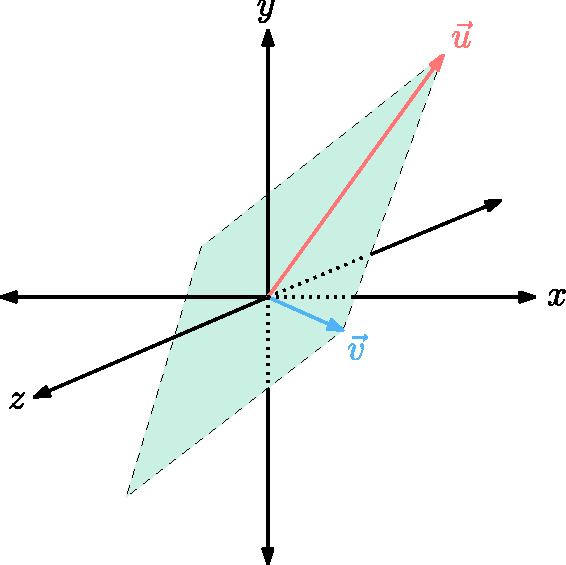
\includegraphics[scale=0.6]{subspaces/plane_in_3d.pdf}
  \end{figure}
\end{frame}

\begin{frame}
  \frametitle{Subspaces}
  And generally, any set of $m<n$ linearly independent vectors in $\Rs{n}$ span a subspace of $\Rs{n}$ which goes through the origin.
\end{frame}

\begin{frame}
  \frametitle{The Dot Product}
  As discussed, any two linearly independent vectors $\rcolor{col1}{\vec{u}},\rcolor{col2}{\vec{v}}\in\Rs{n}$ span a plane which goes through the origin of $\Rs{n}$. In that plane, there is some angle $\rcolor{col4}{\theta}$ between the vectors.

  \begin{figure}[H]
  \centering
  \begin{tikzpicture}
  \Large

  \coordinate (u) at (1,3);
  \coordinate (v) at (3,2);
  \coordinate (uv) at ($(u)+(v)$);
  \filldraw[col4!20, draw=col4, thick] let
  \p1=(u),\p2=(v),\n1={atan2(\y1,\x1)},\n2={atan2(\y2,\x2)}
  in (o) -- ($(o)!1cm!(v)$) arc[start angle=\n2, end angle=\n1, radius=1cm]
  node [text=col4] at ($(o)!7mm!(uv)$) {$\theta$};

  \draw[vector, col1] (o) -- ++(u) node [above right] {$\vec{u}$};
  \draw[vector, col2] (o) -- ++(v) node [above right] {$\vec{v}$};
  \filldraw (o) circle (0.03);
  \end{tikzpicture}
  \end{figure}

  \onslide<2>{
  \centering
  How can we calculate $\rcolor{col4}{\theta}$?
  }
\end{frame}

\begin{frame}
  \frametitle{The Dot Product}
  If we rotate the two vectors such that one of them lies on the horizontal direction, we can draw a perpendicular line from $\rcolor{col1}{\vec{u}}$ to $\rcolor{col2}{\vec{v}}$. Using trigonometry we get
  \begin{equation*}
  \cos(\rcolor{col4}{\theta}) = \frac{\projection}{\vnorm[col1]{u}},
  \end{equation*}
  where $\projection$ is the length of the projection of $\rcolor{col1}{\vec{u}}$ on $\rcolor{col2}{\vec{v}}$.
  \begin{figure}[H]
  \centering
  \begin{tikzpicture}
  \Large

  \coordinate (u) at (2.5,1.94);
  \coordinate (v) at (3.6,0);
  \coordinate (uv) at ($(u)+(v)$);
  \filldraw[col4!20, draw=col4, thick] let
  \p1=(u),\p2=(v),\n1={atan2(\y1,\x1)},\n2={atan2(\y2,\x2)}
  in (o) -- ($(o)!1cm!(v)$) arc[start angle=\n2, end angle=\n1, radius=1cm]
  node [text=col4] at ($(o)!7mm!(uv)$) {$\theta$};

  \draw[vector, col1] (o) -- ++(u) node [above right] {$\vec{u}$};
  \draw[vector, col2] (o) -- ++(v) node [above right] {$\vec{v}$};
  \filldraw (o) circle (0.03);

  \draw[perp, black] (u) -- ++(0,-1.94);
  \filldraw[black] ($(u)+(0,-1.94)$) circle (0.04);
  \draw [black, thick, decorate, decoration={brace, amplitude=3pt, raise=3pt, mirror}]
  (o) -- ($(u)+(0,-1.94)$) node[midway, below , yshift=-5pt]{$\projection$};
  \end{tikzpicture}
  \end{figure}
\end{frame}

\begin{frame}
  \frametitle{The Dot Product}
  We define the magnitude $\projection\cdot\vnorm[col2]{u}$ (i.e. the length of the projection of $\rcolor{col1}{\vec{u}}$ on $\rcolor{col2}{\vec{v}}$ multiplied by the length of $\rcolor{col2}{\vec{v}}$) as the \emph{dot product} of $\rcolor{col1}{\vec{u}}$ and $\rcolor{col2}{\vec{v}}$.

  \onslide<2->{
  Two common notations for the dot product of two vectors $\vec{a},\vec{b}$ are
  \begin{enumerate}
  \item $\vec{a}\cdot\vec{b}$ (the one used in this course), and
  \item $\langle \vec{a},\vec{b} \rangle$.
  \end{enumerate}
  }

  \onslide<3>{
  A more common formulation of the dot product is
  \begin{equation*}
  \rcolor{col1}{\vec{u}} \cdot \rcolor{col2}{\vec{v}} = \vnorm[col1]{u}\vnorm[col2]{v}\cos(\rcolor{col4}{\theta}).
  \end{equation*}
  }
\end{frame}

\begin{frame}
  \frametitle{The Dot Product}
  Some properties of the dot product:
  \begin{itemize}
  \onslide<1->{
  \item It is non-negative, i.e. $\vec{u}\cdot\vec{v}\geq0$.
  }
  \onslide<2->{
  \item It is commutative, i.e. $\vec{u}\cdot\vec{v} = \vec{v}\cdot\vec{u}$.
  }
  \onslide<3->{
  \item It equals zero in only one of two cases:
  \begin{enumerate}
  \onslide<4->{
  \item One of the vectors (or both) is the zero vector, or
  }
  \onslide<5->{
  \item The angle $\theta$ between the vectors is $\ang{90}$ (since then $\cos(\theta)=\cos\left(\ang{90}\right)=0)$.
  }
  \end{enumerate}
  }
  \end{itemize}
\end{frame}

\begin{frame}
  \frametitle{The Dot Product}
  The Last point is so important that it's worth framing it and hanging it on a wall\footnote{Preferably, above your bed so you see it when you wake up and when you go to sleep.}. We will forgoe the hanging part here, and only frame it:

  \onslide<2>{
  \begin{presentation_note}
  \textbf{When the dot product of two (non zero) vectors is equal to zero, they are orthogonal to each other.}
  \begin{equation*}
  \bm{\Updownarrow}
  \end{equation*}
  \textbf{When two (non zero) vectors are orthogonal to each other, their dot product is zero.}
  \end{presentation_note}
  }
\end{frame}

\begin{frame}
  \frametitle{The Dot Product}
  \begin{presentation_example}
  \only<1>{
  What is the dot product of the two vectors $\vec{v}=\colvec{2}{4}{4}$ and $\vec{v}=\colvec{2}{-1}{2}$?

  The angle $\theta$ between $\vec{u}$ and the $x$-axis is
  \begin{equation*}
  \tan(\theta) = \frac{4}{4} = 1 \quad \Rightarrow \quad \theta=\ang{45}.
  \end{equation*}

  The angle $\varphi$ between $\vec{v}$ and the $x$-axis is
  \begin{equation*}
  \tan(\varphi) = \frac{2}{-1} = -2 \quad \Rightarrow \quad \varphi \approx \ang{116.57}.
  \end{equation*}
  }
  
  \only<2>{
  Thus, the angle between the two vectors is $\omega=\varphi-\theta=\ang{71.57}$.

  The norm of $\vec{u}$ is
  \begin{equation*}
  \norm{\vec{u}} = \sqrt{4^{2}+4^{2}} = \sqrt{16+16} = \sqrt{32},
  \end{equation*}
  and of $\vec{v}$ is
  \begin{equation*}
  \norm{\vec{v}} = \sqrt{(-1)^{2}+2^{2}} = \sqrt{1+4} = \sqrt{5}.
  \end{equation*}

  Thus, the dot product of the two vectors is:
  \begin{equation*}
  \vec{u} \cdot \vec{v} = \sqrt{32}\sqrt{5}\cos(\ang{71.57}) = \sqrt{160} \cdot 0.32 = 4.
  \end{equation*}
  }
  \end{presentation_example}
\end{frame}

\begin{frame}
  \frametitle{The Dot Product}
  When two vectors are given as column vectors, their dot product can be calculated as the sum of their component-wise product, i.e.
  \begin{equation*}
  \colvec{4}{a_{1}}{a_{2}}{\vdots}{a_{n}} \cdot \colvec{4}{b_{1}}{b_{2}}{\vdots}{b_{n}} = a_{1}b_{1} + a_{2}b_{2} + \cdots + a_{n}b_{n} = \sum\limits_{i=1}^{n}a_{i}b_{i}.
  \end{equation*}
\end{frame}

\begin{frame}
  \frametitle{The Dot Product}
  \begin{presentation_example}
  Using the vectors $\vec{u}=\colvec{2}{4}{4}$ and $\vec{v}=\colvec{2}{-1}{2}$ from the previous example, we get
  \begin{equation*}
  \vec{u}\cdot\vec{v} = 4\cdot(-1) + 4\cdot2 = -4+8 = 4,
  \end{equation*}
  which is exactly the result we got in the previous example.
  \end{presentation_example}
\end{frame}

\begin{frame}
  \frametitle{The Cross Product}
  Another product of two vectors is the \emph{cross product}. Unlike the dot product, the cross product is only defined on $\Rs{3}$ (and with a somewhat different meaning on $\Rs{2}$ as well).

  \onslide<2->{
  Geometrically, the cross product of two vectors $\rcolor{col1}{\vec{u}}, \rcolor{col2}{\vec{v}} \in \Rs{3}$ is defined as a vector $\rcolor{col4}{\vec{w}}$ which is \textbf{orthogonal to both} $\rcolor{col1}{\vec{u}}$ and $\rcolor{col2}{\vec{v}}$, and has a magnitude
  \begin{equation*}
  \rcolor{col4}{r_{w}} = \vnorm[col1]{u}\vnorm[col2]{v}\sin(\rcolor{col4}{\theta}),
  \end{equation*}
  where $\rcolor{col4}{\theta}$ is the angle between $\rcolor{col1}{\vec{u}}$ and $\rcolor{col2}{\vec{v}}$.
  }
\end{frame}

\begin{frame}
  \frametitle{The Cross Product}
  \begin{figure}[H]
  \centering
  \begin{tikzpicture}
  \huge

  % Plane
  \draw[-, dashed, very thick, fill=col3!30] (0,0,0) -- (0,0,7) -- (7,0,7) -- (7,0,0) -- cycle;
   
  % Coordinates
  \coordinate (o) at (1,0,3);
  \coordinate (u) at (2,0,2.5);
  \coordinate (v) at (4,0,-2);
  \coordinate (w) at (0,3,0);
  
  % Angle
  \draw[very thick, col4, cap=round] (2,0,4.2) arc [start angle=-70, end angle=33, x radius=0.7, y radius=0.4];
  \node[text=col4] at ($(o)+(0.5,-0.13,0)$) {\large$\theta$};

  % Vectors
  \draw[vector, col1] (o) -- ++(u) node [right] {$\vec{u}$};
  \draw[vector, col2] (o) -- ++(v) node [right] {$\vec{v}$};
  \draw[vector, col4] (o) -- ++(w) node [right] {$\rcolor{col4}{\vec{w}}=\rcolor{col1}{\vec{u}}\times\rcolor{col2}{\vec{v}}$};

  % Perpendiculars
  \tikzset{rightangle/.style={-, thick, fill=gray!50, fill opacity=0.5}}
  \draw[rightangle] (o) -- ++(0.3,0,-0.15) -- ++(0,0.3,0) -- ++(-0.3,0,0.15) -- cycle;
  \draw[rightangle] (o) -- ++(0.4,0,0.5) -- ++(0,0.3,0) -- ++(-0.4,0,-0.5) -- cycle;
  \end{tikzpicture}
  \end{figure}
\end{frame}

\begin{frame}
  \frametitle{The Cross Product}
  The direction of $\rcolor{col1}{\vec{u}}\times\rcolor{col2}{\vec{v}}$ is determined by the \emph{right-hand rule}: using a person's right hand, when $\rcolor{col1}{\vec{u}}$ points in the direction of their index finger and $\rcolor{col2}{\vec{v}}$ in the direction of their middle finger, then $\rcolor{col4}{\vec{w}} = \rcolor{col1}{\vec{u}}\times\rcolor{col2}{\vec{v}}$ points in the direction of their thumb:

  \begin{figure}[H]
  \centering
  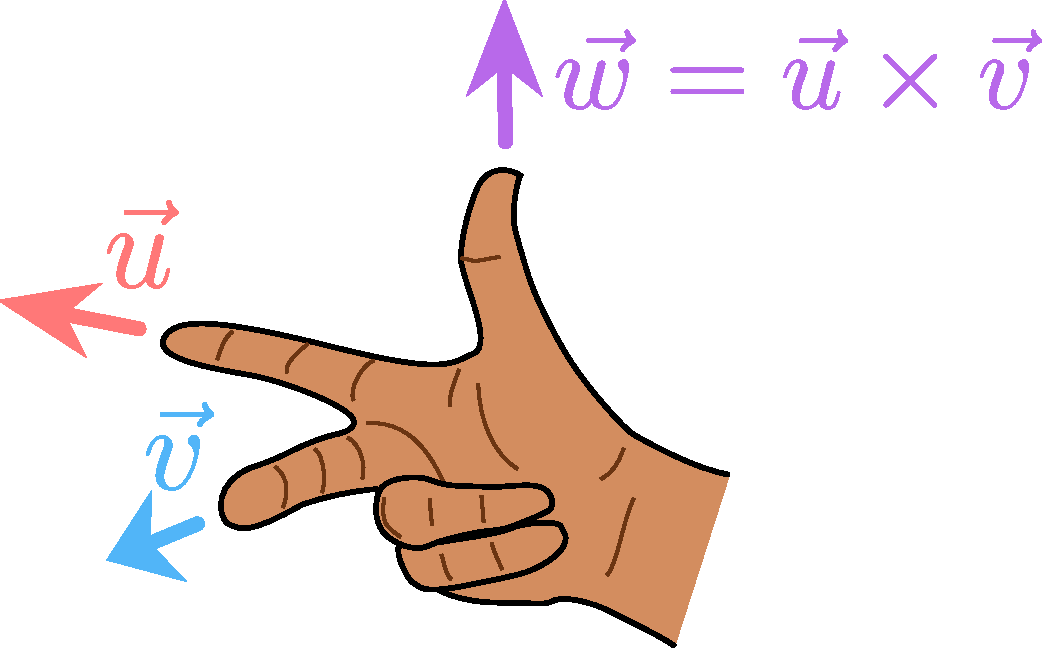
\includegraphics[scale=0.35]{cross_product/rhr.pdf}
  \end{figure}
\end{frame}

\begin{frame}
  \frametitle{The Cross Product}
  The cross product is \emph{anti-commutative}, i.e. changing the order of the vectors results in inverting the product:
  \begin{equation*}
  \rcolor{col1}{\vec{u}}\times\rcolor{col2}{\vec{v}} = -\left( \rcolor{col2}{\vec{v}}\times\rcolor{col1}{\vec{u}} \right).
  \end{equation*}

  \onslide<2>{
  When the vectors are given as column vectors $\rcolor{col1}{\vec{u}}=\colvec{3}{\rcolor{col1}{u_{x}}}{\rcolor{col1}{u_{y}}}{\rcolor{col1}{u_{z}}},\ \rcolor{col2}{\vec{v}}=\colvec{3}{\rcolor{col2}{v_{x}}}{\rcolor{col2}{v_{y}}}{\rcolor{col2}{v_{z}}}$, the resulting cross product is
  \begin{equation*}
  \rcolor{col1}{\vec{u}}\times\rcolor{col2}{\vec{v}} = \begin{pmatrix}\rcolor{col1}{u_{y}}\rcolor{col2}{v_{z}}-\rcolor{col1}{u_{z}}\rcolor{col2}{v_{y}}\\\rcolor{col1}{u_{z}}\rcolor{col2}{v_{x}}-\rcolor{col1}{u_{x}}\rcolor{col2}{v_{z}}\\\rcolor{col1}{u_{x}}\rcolor{col2}{v_{y}}-\rcolor{col1}{u_{y}}\rcolor{col2}{v_{x}}\end{pmatrix}
  \end{equation*}
  }
\end{frame}

\begin{frame}
  \frametitle{The Cross Product}
  \begin{presentation_example}
  What is the cross product of $\eb{1}=\colvec{3}{1}{0}{0}$ and $\eb{2}=\colvec{3}{0}{1}{0}$?
  \begin{equation*}
  \onslide<2->{
  \eb{1}\times\eb{2} = \begin{pmatrix}\cancel{0\cdot0}-\cancel{0\cdot1}\\\cancel{0\cdot0}-\cancel{1\cdot0}\\1\cdot1-\cancel{0\cdot0}\end{pmatrix}
  }
  \onslide<3->{
  = \colvec{3}{0}{0}{1}
  }
  \onslide<4->{
  = \eb{3}.
  }
  \end{equation*}
  \end{presentation_example}
\end{frame}

\begin{frame}
  \frametitle{The Cross Product}
  \begin{presentation_note}
  The cross product of two of the standard basis vectors in $\Rs{3}$ is the third basis vector. Its sign ($\pm$) is determined by a cyclic rule:
  \begin{equation*}
  \text{sign}\left( \eb{i}\times\eb{j} \right) =
  \begin{cases}
  1 & \text{if } (i,j)\in \left\{(1,2),\ (2,3),\ (3,1)\right\},\\
  -1 & \text{if } (i,j)\in \left\{(3,2),\ (2,1),\ (1,3)\right\},\\
  0 & \text{otherwise}.
  \end{cases}
  \end{equation*}
  \end{presentation_note}

  \onslide<2>{
  \begin{presentation_challenge}
  Using component calculation and utilizing the dot product, show that $\pcross{u}{v}$ is indeed orthogonal to both $\vec{u}$ and $\vec{v}$.
  \end{presentation_challenge}
  }
\end{frame}

  \sectionpic{Linear Transformations}{../figures/presentation_chapters/linear_trans.pdf}
\begin{frame}
  \frametitle{Linear Transformations: Definition}
  \begin{presentation_definition}
    A \emph{linear transformation} is a function $\func{T}{A}{B}$, that obeys the following two criteria:
    \begin{enumerate}
        \onslide<2->{
        \item \textbf{Scalability}: for each $x\in A$ and a scalar $\alpha\in\mathbb{R}$:
          \begin{equation*}
            T(\alpha x) = \alpha T(x).
          \end{equation*}
        }
        \onslide<3>{
        \item \textbf{Additivity}: For any $x,y\in A$:
          \begin{equation*}
            T(x+y) = T(x)+T(y).
          \end{equation*}
        }
    \end{enumerate}
  \end{presentation_definition}
\end{frame}

\begin{frame}
  \frametitle{Linear Transformations: Definition}
  \begin{presentation_example}
    The real function $f(x)=3x$ is linear. Proof by the above criteria:
    \begin{enumerate}
        \onslide<2->{
        \item \textbf{Scalability}: for any scalar $\alpha\in\mathbb{R}$, 
          \begin{equation*}
            f(\alpha x)=3(\alpha x)=\alpha \cdot (3x)=\alpha f(x).
          \end{equation*}
        }
        \onslide<3->{
        \item \textbf{Additivity}: for any two numbers $x,y\in\mathbb{R}$
          \begin{equation*}
            f(x+y)=3(x+y)=3x+3y=f(x)+f(y).
          \end{equation*}
        }
    \end{enumerate}
    \onslide<4>{
      Therefore, $f$ is linear.
    }
  \end{presentation_example}
\end{frame}

\begin{frame}
  \frametitle{Linear Transformations: Definition}
  \begin{presentation_example}
    Is the real function $g(x)=3x+5$ linear? Let's check:
    \begin{enumerate}
        \onslide<2->{
        \item \textbf{Scalability}:
          \begin{equation*}
            g(\alpha x) = 3\alpha x + 5,\quad \alpha g(x) = 3x\alpha + 5\alpha.
          \end{equation*}
        }
        \onslide<3->{
          If we subtitute $\alpha=0, x=1$, for example, we get
          \begin{equation*}
            g\left( \alpha x \right)=g\left( 0\cdot1 \right)=\cancel{3\cdot0} + 5=5,
          \end{equation*}
        }
        \onslide<4->{
          but on the other hand
          \begin{equation*}
            \alpha \cdot g(x) = \cancel{3\cdot1\cdot0} + \cancel{5\cdot0} = 0 \neq 5.
          \end{equation*}
        }
        \onslide<5->{
          Therefore, $g$ is \textbf{NOT} linear.
        }
    \end{enumerate}
  \end{presentation_example}
\end{frame}

\begin{frame}
  \frametitle{Linear Transformations: Definition}
  \begin{presentation_note}
    In order to prove that a function is linear, \textbf{both criteria} need to apply to \textbf{all} numbers $\alpha, x,$ and $y$.

    \vspace{5mm}
    \onslide<2->{
      In order to show that a function is \textbf{not} linear, it is enough to show that \textbf{just a single case} doesn't comply with \textbf{any of the criteria}.
    }
  \end{presentation_note}
  \onslide<3>{
    \begin{presentation_challenge}
      Check whether the function $g$ from before complies with the 2nd criterion (additivity).
    \end{presentation_challenge}
  }
\end{frame}

\begin{frame}
  \frametitle{Linear Transformations: Definition}
  \begin{presentation_example}
    Is the function $h(x) = x^{2}$ linear? Let's check additivity first:
    \begin{equation*}
      h(x+y) = (x+y)^{2} = x^{2}+2xy+y^{2}, \quad h(x)+h(y) = x^{2}+y^{2}.
    \end{equation*}
    \onslide<2->{
      Thus, for $x=1,y=-2$:
      \begin{equation*}
        h(x+y) =h(1-2) =h(-1) =(-1)^{2} =1.
      \end{equation*}
    }
    \onslide<3->{
      On the other hand,
      \begin{align*}
        h(x)+h(y)&=h(1)+h(-2)=1^{2} + (-2)^{2}\\&=1+4=5\neq 1.
      \end{align*}
    }
    \onslide<4>{
      Thus, $h$ is also \textbf{NOT} linear.
    }
  \end{presentation_example}
\end{frame}

\begin{frame}
  \frametitle{Linear Transformations: Definition}
  \begin{presentation_challenge}
    Check whether $h$ fulfills the 1st criterion (scalability).
  \end{presentation_challenge}

  \onslide<2->{
    We can combine both criteria to a single test for linearity of a transformation $T$:
    \begin{presentation_definition}
      A transformation $\func{T}{A}{B}$ is linear, if for all $x,y\in A$ and $\alpha,\beta\in\mathbb{R}$ 
      \begin{equation*}
        T\left(\alpha x + \beta y \right) = \alpha T(x) + \beta T(y).
      \end{equation*}
    \end{presentation_definition}
  }
\end{frame}

\begin{frame}
  \frametitle{Transforming Vectors}
  Vectors can also be transformed, specifically by functions of the type $\func{T}{\Rs{n}}{\Rs{m}}$, with $n, m\in\mathbb{N}$.

  \onslide<2->{
    In this course we will mostly concentrate on transformations of the types
  \begin{itemize}
      \item $\func{T}{\Rs{2}}{\Rs{2}}$ and
      \item $\func{T}{\Rs{3}}{\Rs{3}}$.
  \end{itemize}
    since they are more easy to conceptualize (and infintely easier to draw than higher dimensional transformations).
  }

  \onslide<3>{
    However, everything we learn about these transformations is applicable for any linear transformation, \textbf{regardless of its dimensionality}.
  }
\end{frame}

\begin{frame}
  \frametitle{Transforming Vectors}
  \begin{presentation_example}
    Applying the transformation $\func{T}{\Rs{2}}{\Rs{2}}$,
    \begin{equation*}
      T\colvec{2}{\xhl}{\yhl} = \colvec{2}{-\xhl}{3\yhl}
    \end{equation*}
    to the vector $\vec{u}=\colvec{2}{\xhl[3]}{\yhl[1]}$:
    \begin{equation*}
      T\colvec{2}{\xhl[3]}{\yhl[1]} = \colvec{2}{-\xhl[3]}{3\cdot\yhl[1]} = \colvec{2}{-3}{3}.
    \end{equation*}
  \end{presentation_example}
\end{frame}

\begin{frame}
  \frametitle{Transforming Vectors}
  \begin{presentation_example}
    Graphically, the transformation looks as follows:
    \begin{figure}[H]
      \centering
      \begin{tikzpicture}[scale=0.75]
        \Large

        \coordinate (o) at (0,0);
        \coordinate (u) at (3,1);
        \coordinate (Tu) at (-3,3);

        \drawaxes{-4}{-1}{4}{4}

        \draw[vector, col4] (o) --(u) node [above right, yshift=-1mm] {$\vec{v}$};
        \draw[vector, col4!65] (o) --(Tu) node [above] {$T(\vec{v})$};

        \draw[vector, ultra thick, densely dotted, col5!40!col4] (2,1) to [out=120, in=30] node [midway, above, text=col5!40!col4] {$T$} (-1.5,1.75);
        \;
      \end{tikzpicture}
    \end{figure}
  \end{presentation_example}
\end{frame}

\begin{frame}
  \frametitle{Transforming Spaces}
  \only<1>{
    We can visualize the way an entire space is transformed by a transformation $\rcolor{col4}{T}$ by looking at how the axes and main gridlines of the space are transformed.
  }
  \only<2>{
    This method also allows us to see how the basis vectors $\rcolor{col1}{\hat{x}}$ and $\rcolor{col2}{\hat{y}}$ are transformed by linear transformations, and also the transformations of shapes (all this will come in handy later).
  }
  \begin{presentation_example}
    \begin{figure}[H]
      \centering
      \begin{tikzpicture}[scale=0.35]
        \drawaxes{-5}{-5}{5}{5}[0.5][black!50][-][white]
        \only<2>{
          \draw[vector, col1] (0,0) -- (2.5,0);
          \draw[vector, col2] (0,0) -- (0,2.5);
          \draw[col1, thick, fill=col1!50, fill opacity=0.5] (3,2) -- (4,4) -- (2,3) -- cycle;
          \draw[col2, thick, fill=col2!50, fill opacity=0.5] (3,-3) circle (1.2);
          \draw[col3, thick, fill=col3!50, fill opacity=0.5] (-4,4) rectangle (-3,-3);
        }
        \pgftransformcm{1}{0.3}{0.4}{0.7}{\pgfpoint{14cm}{0cm}}
        \drawaxes{-5}{-5}{5}{5}[0.5][black!50][-][white]
        \only<2>{
          \draw[vector, col1] (0,0) -- (2.5,0);
          \draw[vector, col2] (0,0) -- (0,2.5);
          \draw[col1, thick, fill=col1!50, fill opacity=0.5] (3,2) -- (4,4) -- (2,3) -- cycle;
          \draw[col2, thick, fill=col2!50, fill opacity=0.5] (3,-3) circle (1.2);
          \draw[col3, thick, fill=col3!50, fill opacity=0.5] (-4,4) rectangle (-3,-3);
        }
        \pgftransformreset
        \draw[vector, col4] (2,1) -- node[midway, above] {$T$} ++(1.5,0);
      \end{tikzpicture}
    \end{figure}
  \end{presentation_example}
\end{frame}

\begin{frame}
  \frametitle{Properties of Linear Transformations}
  Some important properties of linear transformations are:
  \begin{itemize}
      \onslide<2->{
      \item The origin is preserved, i.e.
        \begin{equation*}
          T\left( \vec{0} \right) = \vec{0}.
        \end{equation*}
      }
      \onslide<3->{
      \item Parallel lines remain parallel.
      }
      \onslide<4->{
      \item All areas are scaled by the same number.
      }
  \end{itemize}
  \onslide<5->{
    \begin{presentation_challenge}
      Show that these properties can be derived from the definition of linear transformations.
    \end{presentation_challenge}
  }
\end{frame}

\begin{frame}
  \frametitle{Types of Linear Transformations}
  Many linear transformations $\func{T}{\Rs{2}}{\Rs{2}}$ can be created by composition of two or more of the following basic transformations:

  \onslide<2->{
    \begin{figure}[H]
      \centering
      \begin{tikzpicture}[scale=0.35]
        \draw[opacity=0] (-6,-5) rectangle (23,11);

        \drawaxes{-5}{-5}{5}{5}[0.5][black!50][-][white]
        \draw[col1, thick, fill=col1!50, fill opacity=0.5] (3,2) -- (4,4) -- (2,3) -- cycle;
        \draw[col2, thick, fill=col2!50, fill opacity=0.5] (3,-3) circle (1.2);
        \draw[col3, thick, fill=col3!50, fill opacity=0.5] (-4,4) rectangle (-3,-3);

        \only<2> \pgftransformcm{0.7}{0}{0}{1}{\pgfpoint{14cm}{0cm}}
        \only<3> \pgftransformcm{1}{0}{0}{0.5}{\pgfpoint{16cm}{0cm}}
        \only<4> \pgftransformcm{0.87}{0.5}{-0.5}{0.87}{\pgfpoint{16cm}{0cm}}
        \only<5> \pgftransformcm{1}{0}{0.3}{1}{\pgfpoint{16cm}{0cm}}
        \only<6> \pgftransformcm{1}{-0.5}{0}{1}{\pgfpoint{16cm}{0cm}}
        \only<7> {
          \draw[-, densely dotted, col4, very thick] (-5,-5) -- (5,5);
          \pgftransformcm{0}{1}{1}{0}{\pgfpoint{16cm}{0cm}}
          \draw[-, densely dotted, col4, very thick] (-5,-5) -- (5,5);
        }

        \drawaxes{-5}{-5}{5}{5}[0.5][black!50][-][white]
        \draw[col1, thick, fill=col1!50, fill opacity=0.5] (3,2) -- (4,4) -- (2,3) -- cycle;
        \draw[col2, thick, fill=col2!50, fill opacity=0.5] (3,-3) circle (1.2);
        \draw[col3, thick, fill=col3!50, fill opacity=0.5] (-4,4) rectangle (-3,-3);

        \pgftransformreset

        \draw[vector, col4] (2,1) -- node[midway, above] (T) {$T$} ++(1.5,0);
        \node[above=of T, yshift=5mm] {
          \only<2>{Scaling in the $x$-axis}
          \only<3>{Scaling in the $y$-axis}
          \only<4>{Rotation around the origin}
          \only<5>{Shear in the $x$-axis}
          \only<6>{Shear in the $y$-axis}
          \only<7>{Reflection by a line going through the origin}
        };
      \end{tikzpicture}
    \end{figure}
  }
\end{frame}

\begin{frame}
  \frametitle{Types of Linear Transformations}
  \begin{presentation_example}
    The following transformation is a composition of a scaling transformation in the $y$-axis, followed by a rotation around the origin:
    \begin{figure}[H]
      \centering
      \begin{tikzpicture}[scale=0.35]
      \end{tikzpicture}
    \end{figure}
  \end{presentation_example}
\end{frame}

  \sectionpic{Matrices}{../figures/presentation_chapters/matrices.pdf}
\begin{frame}
  \frametitle{Matrices from Linear Transformations}
  Any vector in a space $\Rs{n}$ can be written as a linear combination of the elements of a base in $\Rs{n}$.
  \onslide<2->{
    \begin{presentation_example}
      The vector $\colvec{2}{1}{-3}$ can be written as a linear combination of the standard basis vectors in $\Rs{2}$:
      \begin{align*}
        \onslide<3->{\vec{v} &= \colvec{2}{1}{0} + \colvec{2}{0}{-3}\\}
        \onslide<4->{&= \colvec{2}{1}{0} -3\colvec{2}{0}{1}\\}
        \onslide<5->{&= \eb{1} -3\eb{2}\\}
        \onslide<6->{&= \hat{x} -3\hat{y}.}
      \end{align*}
    \end{presentation_example}
  }
\end{frame}

\begin{frame}
  \frametitle{Matrices from Linear Transformations}
  When a linear transformation $T$ is applied to a vector $\vec{v}=\alpha_{1}\eb{1} + \alpha_{2}\eb{2} + \cdots + \alpha_{n}\eb{n}$, linearity dictates the following:
  \begin{align*}
    \onslide<2->{T\left( \vec{v} \right) &= T\left( \alpha_{1}\eb{1} + \alpha_{2}\eb{2} + \cdots + \alpha_{n}\eb{n} \right)\\}
    \onslide<3->{&\ \tikznode{add}{=}\ T\left( \alpha_{1}\eb{1} \right) + T\left( \alpha_{2}\eb{2} \right) + \cdots + T\left( \alpha_{n}\eb{n} \right)\\}
    \onslide<4->{&\ \tikznode{scl}{=}\ \alpha_{1}T\left( \eb{1} \right) + \alpha_{2}T\left( \eb{2} \right) + \cdots + \alpha_{n}T\left( \eb{n} \right),}
  \end{align*}
  \begin{tikzpicture}[overlay, remember picture]
    \onslide<3->{
      \node[nodehl, left=of add, draw=col1, fill=col1!20] (addtxt) {Additivity};
      \draw[arrowhl, col1] (addtxt.east) -- (add.west);
    }
    \onslide<4->{
      \node[nodehl, left=of scl, draw=col2, fill=col2!20] (scltxt) {Scalability};
      \draw[arrowhl, col2] (scltxt.east) -- (scl.west);
    }
  \end{tikzpicture}

  \onslide<5->{
    i.e. - the transformed vector is a linear combination of the transformed standard basis vectors, with the components of the original vector as coefficients.
  }
\end{frame}

\begin{frame}
  \frametitle{Matrices from Linear Transformations}
  \begin{presentation_example}
    \only<1>{
      Consider the vector $\vec{v}=\colvec{2}{3}{-1}$, and the transformation $T\colvec{2}{\xhl}{\yhl} = \colvec{2}{-2\xhl+\yhl}{3\xhl-2\yhl}$. We can calculate the transformation $T\left( \vec{v} \right)$ directly:
      \begin{equation*}
        T\left( \vec{v} \right) = \colvec{2}{-2(\xhl[3])+(\yhl[-1])}{3(\xhl[3])-2(\yhl[-1])} = \colvec{2}{-6-1}{9+2} = \colvec{2}{-7}{11}.
      \end{equation*}
    }
    \only<2->{
      Alternatively, we can first look at how the transformation affects the basis vectors $\eb{1}$ and $\eb{2}$:
      \begin{align*}
        \onslide<3->{
          T\left( \eb{1} \right) &= T\colvec{2}{\xhl[1]}{\yhl[0]} = \colvec{2}{-2(\xhl[1])+1(\yhl[0])}{3(\xhl[1])-2(\yhl[0])} = \colvec{2}{-2}{3},\\
        }
        \onslide<4->{
          T\left( \eb{2} \right) &= T\colvec{2}{\xhl[0]}{\yhl[1]} = \colvec{2}{-2(\xhl[0])+1(\yhl[1])}{3(\xhl[0])-2(\yhl[1])} = \colvec{2}{1}{-2}.\\
        }
      \end{align*}

      \onslide<5->{
        \vspace{-1cm}
        Thus, $T$ applied to $\vec{v}=\colvec{2}{3}{-1}$ is
        \begin{align*}
          T\left( \vec{v} \right) &= 
          \onslide<6->{\xhl[3]\colvec{2}{-2}{3} - \yhl[1]\colvec{2}{1}{-2}}
          \onslide<7->{= \colvec{2}{-6}{9} - \colvec{2}{1}{-2}}
          \onslide<8->{= \colvec{2}{-7}{11}.}
        \end{align*}
      }
    }
  \end{presentation_example}
\end{frame}

\begin{frame}
  \frametitle{Matrices from Linear Transformations}
  Generalizing this for any vector $\vec{v}=\colvec{2}{x}{y}\in\Rs{2}$ yields
  \begin{equation*}
    T\colvec{2}{x}{y} = \colvec{2}{ax+by}{cx+dy},
  \end{equation*}
  where $a,b,c,d\in\mathbb{R}$.

  This form of writing a linear transformation applied to a vector has a nice structure: the first component of the resulting vector is the dot product
  \begin{equation*}
    \colvec{2}{a}{b} \cdot \colvec{2}{x}{y},
  \end{equation*}
  while the second component is the dot product
  \begin{equation*}
    \colvec{2}{c}{d} \cdot \colvec{2}{x}{y}.
  \end{equation*}
\end{frame}

\begin{frame}
  \frametitle{Matrices from Linear Transformations}
  We can collect the coefficients $a,b,c$ and $d$ together to a compact structure called a \emph{matrix}:
  \begin{equation*}
    M = \begin{pmatrix} a & b \\ c & d \end{pmatrix}.
  \end{equation*}

  Then, we can define the product of that matrix with a vector $\vec{v}=\colvec{2}{x}{y}$ as
  \begin{equation*}
    M\cdot\vec{v} = \begin{pmatrix} a & b \\ c & d \end{pmatrix}\colvec{2}{x}{y} = \colvec{2}{ax+by}{cx+dy}.
  \end{equation*}
\end{frame}

\begin{frame}
  \frametitle{Matrices from Linear Transformations}
  \begin{presentation_note}
    In the matrix
    \begin{equation*}
      M = \begin{pmatrix} a & b \\ c & d \end{pmatrix},
    \end{equation*}
    The column $\colvec{2}{a}{c}$ shows us how $\eb{1}$ is transformed by the matrix $M$, while the column $\colvec{2}{b}{d}$ shows us how $\eb{2}$ is transformed by the matrix.
  \end{presentation_note}
\end{frame}

\begin{frame}
  \frametitle{Matrices from Linear Transformations}
  Of course, this can be generalized to any transformation $\func{T}{\Rs{n}}{\Rs{n}}$ as
  \begin{equation*}
    M = \begin{pmatrix}
      \onslide<2>{\tmi{3}{eb1}}\mel[a][1][1] & \onslide<2>{\tmi{4}{eb2}}\mel[a][1][2] & \cdots & \onslide<2>{\tmi{5}{ebn}}\mel[a][1][n]\\
      \mel[a][2][1] & \mel[a][2][2] & \cdots & \mel[a][2][n]\\
      \vdots & \vdots & \ddots & \vdots\\
      \mel[a][n][1]\onslide<2>{\tikzmarkend{eb1}} & \mel[a][n][2]\onslide<2>{\tikzmarkend{eb2}} & \cdots & \mel[a][n][n]\onslide<2>{\tikzmarkend{ebn}}
    \end{pmatrix}.
  \end{equation*}

  \onslide<2>{
    \begin{tikzpicture}[overlay, remember picture,
        every node/.style={nodehl, text=black, xshift=3.5mm, yshift=-7mm},
      every path/.style={arrowhl}]
      \tiny
      \node[above=of eb1, draw=col3, fill=col3!20] (eb1txt) {$T\left(\eb{1}\right)$};
      \node[above=of eb2, draw=col4, fill=col4!20] (eb2txt) {$T\left(\eb{2}\right)$};
      \node[above=of ebn, draw=col5, fill=col5!20] (ebntxt) {$T\left(\eb{n}\right)$};

      \draw[col3] (eb1txt.south) -- ($(eb1.north)+(3.5mm,-1mm)$);
      \draw[col4] (eb2txt.south) -- ($(eb2.north)+(3.5mm,-1mm)$);
      \draw[col5] (ebntxt.south) -- ($(ebn.north)+(3.5mm,-1mm)$);
    \end{tikzpicture}
  }

  The numbers $\mel$ are called the \emph{elements} of the Matrix, where $\xhl[i]$ is the \textbf{row} of the element, and $\yhl[j]$ is the \textbf{column} of the element.

  \onslide<2>{
    In addition, each column of the matrix tells us how the respective standard basis vector is transformed.
  }
\end{frame}

\begin{frame}
  \frametitle{Matrices from Linear Transformations}
  \begin{presentation_example}
    The transformation $\func{T}{\Rs{3}}{\Rs{3}}$ which scales space by $2$ in the $x$-direction, by $0.75$ in the $y$-direction and by $1.5$ in the $z$-direction, transforms the standard basis vectors $\hat{x}, \hat{y}$ and $\hat{z}$ as following:
    \onslide<2->{
      \begin{equation*}
        T\left( \hat{x} \right) = \colvec{3}{2}{0}{0},\ 
        T\left( \hat{y} \right) = \colvec{3}{0}{0.75}{0},\ 
        T\left( \hat{z} \right) = \colvec{3}{0}{0}{1.5}.
      \end{equation*}
    }
    \onslide<3->{
      Thus, the corresponding matrix $M$ is
      \begin{equation*}
        M = \begin{pmatrix}
          2 & 0 & 0\\
          0 & 0.75 & 0\\
          0 & 0 & 1.5
        \end{pmatrix}.
      \end{equation*}
    }
  \end{presentation_example}
\end{frame}

\begin{frame}
  \frametitle{Matrices from Linear Transformations}
  Generalizing even further, a matrix representing a linear transformation of a type $\func{T}{\Rs{n}}{\Rs{m}}$ is constructed from $n$ column vectors, each of $m$ components:
  \onslide<2>{
    \begin{equation*}
      M = \begin{pmatrix}
        \mel[a][1][1] & \mel[a][1][2] & \cdots & \mel[a][1][n]\tikznode{v}{}\\
        \mel[a][2][1] & \mel[a][2][2] & \cdots & \mel[a][2][n]\\
        \vdots & \vdots & \ddots & \vdots\\
        \tikznode{h}{}a_{\xhl[m]\yhl[1]} & a_{\xhl[m]\yhl[2]} & \cdots & a_{\xhl[m]\yhl[n]}\tikznode{e}{}
      \end{pmatrix}
    \end{equation*}
    \begin{tikzpicture}[overlay, remember picture]
      \draw[annotation, draw=col2, thick, cap=round, decorate, decoration={brace, amplitude=3pt, raise=5mm, mirror}]
      (h) -- (e) node[annotationtext, midway, yshift=-1cm, col2] {$n$ column vectors};
      \draw[annotation, draw=col1, thick, cap=round, decorate, decoration={brace, amplitude=3pt, raise=5mm}]
      ($(v)+(1mm,3mm)$) -- ($(e)+(0,-3mm)$) node[annotationtext, midway, xshift=2.4cm, text width=3cm, col1] {$m$ components per vector};
    \end{tikzpicture}
  }
\end{frame}

\begin{frame}
  \frametitle{Matrices from Linear Transformations}
  \begin{presentation_example}
    The matrix
    \begin{equation*}
      M = \begin{pmatrix}
        1 & -3 & 7\\
        2 & 0 & -5
      \end{pmatrix}
    \end{equation*}
    takes vectors in $\Rs{3}$ and transforms them to vectors in $\Rs{2}$.

    For example,
    \begin{align*}
      M\cdot\colvec{3}{\xhl[1]}{\yhl[2]}{\zhl[3]} &= \colvec{2}{1\cdot\xhl[1] -3\cdot\yhl[2] + 7\cdot\zhl[3]}{2\cdot\xhl[1] + 0\cdot\yhl[2] - 5\cdot\zhl[3]}\\
      &= \colvec{2}{1-6+21}{2-15} = \colvec{2}{16}{-13}.
    \end{align*}
  \end{presentation_example}
\end{frame}

\setbeamertemplate{background}{\begin{tikzpicture}[overlay, remember picture]
    \draw[-, line width=5mm, cap=round, col3, opacity=0.35]
    ([xshift=0.5ex]start.north west) -- ([xshift=-0.5ex]end.south east);
\end{tikzpicture}}
\begin{frame}
  \frametitle{Types of Matrices}
  A matrix which represents a linear transformation $\func{T}{\Rs{n}}{\Rs{n}}$ is called a \emph{square matrix} (since it has $n\times n$ elements, i.e. $n$ rows and $n$ columns).

  In a square matrix, the elements $\mel[a][1][1],\mel[a][2][2],\dots,\mel[a][n][n]$ are called together the \emph{principal diagonal} (also \emph{main diagonal}) of the matrix.
  \begin{equation*}
    \begin{pmatrix}
      \tikznode{start}{\mel[a][1][1]} & \mel[a][1][2] & \cdots & \mel[a][1][n]\\
      \mel[a][2][1] & \mel[a][2][2] & \cdots & \mel[a][n][n]\\
      \vdots & \vdots & \ddots & \vdots\\
      \mel[a][n][1] & \mel[a][n][2] & \cdots & \tikznode{end}{\mel[a][n][n]}\\
    \end{pmatrix}
  \end{equation*}
\end{frame}
\setbeamertemplate{background}{}

\begin{frame}
  \frametitle{Types of Matrices}
  %write: minor diagonal, diagonal matrix, upper/lower triangular matrix, trace.
  %(also add at some place in the beginning something about matrix notation)
  A \emph{diagonal matrix} is a matrix in which any element outside the main diagonal is zero.
  \begin{presentation_example}
    Some diagonal matrices:
    \begin{equation*}
      \begin{pmatrix} 1 & 0 \\ 0 & -3 \end{pmatrix},\quad
      \begin{pmatrix} -4 & 0 & 0 \\ 0 & 2 & 0 \\ 0 & 0 & 5 \end{pmatrix},\quad
      \begin{pmatrix} 1 & 0 & 0 & 0 \\ 0 & 3 & 0 & 0 \\ 0 & 0 & 3 & 0 \\ 0 & 0 & 0 & 7 \end{pmatrix}.
    \end{equation*}
  \end{presentation_example}
\end{frame}

\begin{frame}
  \frametitle{Types of Matrices}
  An \emph{upper triangular matrix} is a matrix in which all the elements \textbf{below} the main diagonal are equal to zero.
  
  Similarily, a \emph{lower triangular matrix} is a matrix in which all the elements \textbf{above} the main diagonal are equal to zero.
\end{frame}

\begin{frame}
  \frametitle{Types of Matrices}
  \begin{presentation_example}
    An upper triangular matrix:
    \begin{equation*}
      \begin{pmatrix}
        1 & 4 & 3 & -1 \\
        0 & 2 & 3 & -1 \\
        0 & 0 & 7 & 7 \\
        0 & 0 & 0 & -2 \\
      \end{pmatrix}
    \end{equation*}

    A lower triangular matrix:
    \begin{equation*}
      \begin{pmatrix}
        -1 & 0 & 0 & 0 \\
        2 & 5 & 0 & 0 \\
        6 & 4 & 7 & 0 \\
        1 & 0 & 3 & -2 \\
      \end{pmatrix}
    \end{equation*}
  \end{presentation_example}
\end{frame}

\begin{frame}
  \frametitle{Trace}
	The \emph{trace} of a square matrix is the sum of its main diagonal elements, i.e. for an $n\times n$ matrix $A$ with elements $a_{\xhl[i]\yhl[j]}$,
  \begin{equation*}
		\tr(A) = \sum\limits_{i=1}^{n} a_{\xhl[i]\yhl[i]}.
  \end{equation*}
  \begin{presentation_example}
    The trace of
    \begin{equation*}
      A =
      \begin{pmatrix}
        1 & 0 & 2 & -5\\
        5 & 3 & 1 & 2\\
        -4 & 9 & 3 & -1\\
        1 & 0 & 2 & 7\\
      \end{pmatrix}
    \end{equation*}
    is $1+3+3+7=14$.
  \end{presentation_example}
\end{frame}

\begin{frame}
  \frametitle{Transposing Matrices}
  An important operator that can be applied to matrices is the \emph{transpose}. The transpose exchanges the rows of the matrix with its columns, i.e.
  \begin{equation*}
    \mel \xrightarrow[] {\text{transpose}} \mel[a][j][i].
  \end{equation*}

  The notation for the transpose of a matrix $A$ is $A^{\top}$.
\end{frame}

\begin{frame}
  \frametitle{Transposing Matrices}
  \begin{presentation_example}
    \begin{align*}
      \begin{pmatrix}
        \xhl[1] & \whl[2] & \whl[3]\\
        \zhl[4] & \xhl[5] & \whl[6]\\
        \zhl[7] & \zhl[8] & \xhl[9]\\
      \end{pmatrix}^{\top}&=
      \begin{pmatrix}
        \xhl[1] & \zhl[4] & \zhl[7]\\
        \whl[2] & \xhl[5] & \zhl[8]\\
        \whl[3] & \whl[6] & \xhl[9]\\
      \end{pmatrix},\\[5mm]
      \begin{pmatrix}
        \zhl[0] & \zhl[1] & \zhl[-1]\\
        \whl[2] & \whl[-3] & \whl[5]
      \end{pmatrix}^{\top}&=
      \begin{pmatrix}
        \zhl[0]  & \whl[2]\\
        \zhl[1]  & \whl[-3]\\
        \zhl[-1] & \whl[5]
      \end{pmatrix}.
    \end{align*}
  \end{presentation_example}
\end{frame}

\begin{frame}
  \frametitle{Transposing Matrices}
  \onslide<1->{
    \begin{presentation_note}
      In square matrices, the main diagonal elements stay at the same place when the matrix is transposed (since $\mel[a][i][i] = \mel[a][i][i]$). This also means that $\tr(A) = \tr\left( A^{\top} \right)$.
    \end{presentation_note}
  }
  \onslide<2>{
    \begin{presentation_note}
      The transpose of a transposed matrix is the original matrix, i.e.
      \begin{equation*}
        \left( A^{\top}\right )^{\top} = A.
      \end{equation*}
    \end{presentation_note}
  }
\end{frame}

\begin{frame}
  \frametitle{Adding Matrices}
  Like with vectors, addition of two matrices is done element-wise, i.e.
  \begin{align*}
    &\begin{pmatrix}
      \mel[a][1][1] & \mel[a][1][2] & \cdots & \mel[a][1][m]\\
      \mel[a][2][1] & \mel[a][2][2] & \cdots & \mel[a][2][m]\\
      \vdots & \vdots & \ddots & \vdots\\
      \mel[a][n][1] & \mel[a][n][2] & \cdots & \mel[a][n][m]
    \end{pmatrix} + 
    \begin{pmatrix}
      \mel[b][1][1] & \mel[b][1][2] & \cdots & \mel[b][1][m]\\
      \mel[b][2][1] & \mel[b][2][2] & \cdots & \mel[b][2][m]\\
      \vdots & \vdots & \ddots & \vdots\\
      \mel[b][n][1] & \mel[b][n][2] & \cdots & \mel[b][n][m]
    \end{pmatrix} =\\
    &\begin{pmatrix}
      \mel[a][1][1] + \mel[b][1][1] & \mel[a][1][2] + \mel[b][1][2] & \cdots & \mel[a][1][m] + \mel[b][1][m]\\
      \mel[a][2][1] + \mel[b][2][1] & \mel[a][2][2] + \mel[b][2][2] & \cdots & \mel[a][2][m] + \mel[b][2][m]\\
      \vdots & \vdots & \ddots & \vdots\\
      \mel[a][n][1] + \mel[b][n][1] & \mel[a][n][2] + \mel[b][n][2] & \cdots & \mel[a][n][m] + \mel[b][n][m]
    \end{pmatrix}.
  \end{align*}
\end{frame}

\begin{frame}
  \frametitle{Adding Matrices}
  \begin{presentation_example}
    \begin{align*}
      \begin{pmatrix}
        1 & 3 & -7\\
        2 & 0 & 1\\
        0 & -4 & 5
      \end{pmatrix} +
      \begin{pmatrix}
        0 & -2 & 1\\
        3 & 2 & 3\\
        5 & 6 & -1
      \end{pmatrix} &=
      \begin{pmatrix}
        1 & 1 & -6\\
        5 & 2 & 4\\
        5 & 2 & 4
      \end{pmatrix},\\[5mm]
      \begin{pmatrix}
        2 & -1 & 0\\
        1 & 5 & 9
      \end{pmatrix} +
      \begin{pmatrix}
        1 & 3 & 1\\
        0 & 0 & 1
      \end{pmatrix} &=
      \begin{pmatrix}
        3 & 2 & 1\\
        1 & 5 & 10
      \end{pmatrix}.
    \end{align*}
  \end{presentation_example}
\end{frame}

\begin{frame}
  \frametitle{Multiplying a Matrix by a Scalar}
  Also like with vectors, multiplying a matrix $A$ by a scalar $\alpha$ results in multiplying each element $\mel$ of the matrix by $\alpha$, i.e.
  \begin{equation*}
    \alpha\cdot\begin{pmatrix}
      \mel[a][1][1] & \mel[a][1][2] & \cdots & \mel[a][1][m]\\
      \mel[a][2][1] & \mel[a][2][2] & \cdots & \mel[a][2][m]\\
      \vdots & \vdots & \ddots & \vdots\\
      \mel[a][n][1] & \mel[a][n][2] & \cdots & \mel[a][n][m]
    \end{pmatrix} = 
    \begin{pmatrix}
      \mel[\alpha \cdot a][1][1] & \mel[\alpha \cdot a][1][2] & \cdots & \mel[\alpha \cdot a][1][m]\\
      \mel[\alpha \cdot a][2][1] & \mel[\alpha \cdot a][2][2] & \cdots & \mel[\alpha \cdot a][2][m]\\
      \vdots & \vdots & \ddots & \vdots\\
      \mel[\alpha \cdot a][n][1] & \mel[\alpha \cdot a][n][2] & \cdots & \mel[\alpha \cdot a][n][m]
    \end{pmatrix}.
  \end{equation*}
\end{frame}

\begin{frame}
  \frametitle{Adding Matrices}
  \begin{presentation_example}
    \begin{align*}
      5\cdot\begin{pmatrix}
        1 & 3 & -7\\
        2 & 0 & 1\\
        0 & -4 & 5
      \end{pmatrix} &=
      \begin{pmatrix}
        5 & 15 & -35\\
        10 & 0 & 5\\
        0 & -20 & 25
      \end{pmatrix},\\[5mm]
      -\frac{1}{2}\cdot\begin{pmatrix}
        2 & -6 & 2\\
        0 & 0 & -2
      \end{pmatrix} &=
      \begin{pmatrix}
        -1 & 3 & -1\\
        0 & 0 & 1
      \end{pmatrix}.
    \end{align*}
  \end{presentation_example}
\end{frame}

\begin{frame}
  \frametitle{The Identity Matrix}
  Since the columns in a matrix represent the transformation of the standard basis vectors, a matrix which is composed from the standard basis vectors in their original order does not change the space at all. We call such a matrix the \emph{identity matrix}, denoted by $I_{n}$, where $n$ is the dimentionality of the space.
  \begin{equation*}I_{n}=
    \begin{pmatrix}
      1 & 0 & \cdots & 0\\
      0 & 1 & \cdots & 0\\
      \vdots & \vdots & \ddots & \vdots\\
      0 & 0 & \cdots & 1\\
    \end{pmatrix}.
  \end{equation*}
\end{frame}

\begin{frame}
  \frametitle{The Identity Matrix}
  \begin{presentation_example}
    \begin{equation*}
      I_{2} = \begin{pmatrix}
        1 & 0\\
        0 & 1
      \end{pmatrix},\ 
      I_{3} = \begin{pmatrix}
        1 & 0 & 0 \\
        0 & 1 & 0 \\
        0 & 0 & 1
      \end{pmatrix},\ 
      I_{4} = \begin{pmatrix}
        1 & 0 & 0 & 0 \\
        0 & 1 & 0 & 0 \\
        0 & 0 & 1 & 0 \\
        0 & 0 & 0 & 1
      \end{pmatrix},\dots
    \end{equation*}
  \end{presentation_example}
\end{frame}

\begin{frame}
  \frametitle{The Identity Matrix}
  A shorthand way of writing the elements of the identity matrix is by using the \emph{Kronecker delta}, which is defined as
  \begin{equation*}
    \mel[\delta][i][j] = \begin{cases}
      1 & \text{if } \xhl[i]=\yhl[j],\\
      0 & \text{if } \xhl[i]\neq \yhl[j].
    \end{cases}
  \end{equation*}
\end{frame}

\begin{frame}
  \frametitle{Basic Matrices}
  Let's now go over the basic linear transformations $\func{T}{\Rs{2}}{\Rs{2}}$ mentioned in the previous chapter and construct a matrix for each one.

    We will construct each matrix by looking at what effects does the respective transformation have on the basis vectors $\hat{x}=\colvec{2}{1}{0}$ and $\hat{y}=\colvec{2}{0}{1}$, and then joining them together to form the matrix.

    When possible, we will generalize to $\Rs{n}$.
\end{frame}

\begin{frame}
  \frametitle{Scaling Matrices}
  \textbf{Scaling in the $x$- and $y$-axes}

  Scaling in the $x$-axis by $\alpha$ should transform $\hat{x}$ to $\colvec{2}{\alpha}{0}$.\\
  Similarily, scaling in the $y$-axis by $\beta$ should transform $\hat{y}$ to $\colvec{2}{0}{\beta}$.

  \begin{figure}[H]
    \centering
    \begin{tikzpicture}
      \coordinate (o) at (0,0);
      \coordinate (xhat) at (1,0);
      \coordinate (yhat) at (0,1);
      \xaxis{-4}{4}
      \yaxis{-1}{3}
      \draw[vector, col4] (o) -- ($3*(xhat)$) node [above] {$\alpha\hat{x}=\colvec{2}{\alpha}{0}$};
      \draw[vector, col3] (o) -- ($2*(yhat)$) node [left] {$\beta\hat{y}=\colvec{2}{0}{\beta}$};
      \xhat
      \yhat
    \end{tikzpicture}
  \end{figure}
\end{frame}

\begin{frame}
  \frametitle{Scaling Matrices}
  Thus, a general scaling matrix in $\Rs{2}$ is
  \begin{equation*}
    S = \begin{pmatrix} \alpha & 0 \\ 0 & \beta \end{pmatrix}.
  \end{equation*}

  \onslide<2->{
    This can be generalized to $\Rs{n}$ as a diagonal matrix
    \begin{equation*}
      S = \begin{pmatrix}
        s_{1} & 0 & \cdots & 0\\
        0 & s_{2} & \cdots & 0\\
        \vdots & \vdots & \ddots & \vdots\\
        0 & 0 & \cdots & s_{n}\\
      \end{pmatrix}
    \end{equation*}
  }
\end{frame}

\begin{frame}
  \frametitle{Rotation Matrices}
  When rotating $\hat{x}$ by an angle $\theta$, we get a vector that has norm $1$ (because rotation doesn't change the norm) and thus the components
  \begin{align*}
    x &= \cos(\theta),\\
    y &= \sin(\theta).
  \end{align*}

  \begin{figure}[H]
    \centering
    \begin{tikzpicture}[scale=3]
      \coordinate (Tx) at (0.71,0.71);
      \coordinate (Txp) at ($0.7*(xhat)+0.3*(Tx)$);
      \filldraw[col4!20, draw=col4, thick] let
      \p1=(Tx), \p2=(xhat), \n1={atan2(\y1,\x1)}, \n2={atan2(\y2,\x2)}
      in (o) -- ($(o)!.25cm!(xhat)$) arc[start angle=\n2, end angle=\n1, radius=.25cm]
      node [text=col4] at ($(o)!.17cm!(Txp)$) {$\theta$};
			\draw[vector, col4] (o) -- (Tx)  node [above] {$A\cdot\hat{x}$} node [midway, above] (1) {};
      \draw[perp] (Tx) -- (Tx|-xhat);
      \draw [col1, thick, decorate, decoration={brace, amplitude=3pt, raise=3pt, mirror}]
      (o) -- (Tx|-xhat) node[midway, below , yshift=-5pt]{$\cos(\theta)$};
      \draw [col2, thick, decorate, decoration={brace, amplitude=3pt, raise=3pt, mirror}]
      (Tx|-xhat) -- (Tx) node[midway, right , xshift=5pt]{$\sin(\theta)$};
      \xaxis{-0.2}{1}
      \yaxis{-0.2}{1}
			\node[nodehl, above left=of 1, xshift=5mm, yshift=-5mm, col4, fill=col4!30] (1txt) {norm=$1$};
			\draw[vector, thick, col4!30] (1txt.south) to [out=-90, in=135] (1);
    \end{tikzpicture}
  \end{figure}
\end{frame}

\begin{frame}
  \frametitle{Rotation Matrices}
  Since $\hat{y}$ is $\ang{90}$ "ahead" of $\hat{x}$ (i.e. its angle to the $x$-axis is always $\ang{90}$ more than that of $\hat{x}$), we excpet the rotated $\hat{y}$ to have the components
  \begin{align*}
    x &= \cos\left( \theta+\ang{90} \right),\\
    y &= \sin\left( \theta+\ang{90} \right).\\
  \end{align*}

  Two trigonometric identities come in handy:
  \begin{enumerate}
    \item $\cos\left( \theta+\ang{90} \right) = -\sin(\theta)$, and
    \item $\sin\left( \theta+\ang{90} \right) = \cos(\theta)$.
  \end{enumerate}

  Thus, $\hat{y}$ transforms to $\colvec{2}{-\sin(\theta)}{\cos(\theta)}$.
\end{frame}

\begin{frame}
  \frametitle{Rotation Matrices}
  Alltogether, in $\Rs{2}$ the matrix representing a counter clock-wise rotation by $\theta$ around the origin is
  \begin{equation*}
    \Rot(\theta) = \RotMat.
  \end{equation*}
\end{frame}

\begin{frame}
  \frametitle{Rotation Matrices}
  \begin{presentation_example}
    Rotation by $\ang{45}$ around the origin is given by
    \begin{equation*}
      \Rot\left( \ang{45} \right) = \RotMat[\ang{45}][\ang{45}][\ang{45}][\ang{45}]
      = \begin{pmatrix}
        \frac{2}{\sqrt{2}} & -\frac{2}{\sqrt{2}}\\
        \frac{2}{\sqrt{2}} & \frac{2}{\sqrt{2}}
      \end{pmatrix}.
    \end{equation*}

    Applying this to the vector $\vec{v}=\colvec{2}{1}{3}$ results in
    \begin{align*}
      \vec{u}=
      \Rot\left( \ang{45} \right)\cdot\vec{v}
      &= \begin{pmatrix}
        \frac{2}{\sqrt{2}} & -\frac{2}{\sqrt{2}}\\
        \frac{2}{\sqrt{2}} & \frac{2}{\sqrt{2}}
      \end{pmatrix}\colvec{2}{1}{3}
      = \frac{\sqrt{2}}{2}\colvec{2}{1-3}{1+3}\\
      &= \frac{\sqrt{2}}{2}\colvec{2}{-2}{4}
      = \colvec{2}{-\sqrt{2}}{2\sqrt{2}}.
    \end{align*}
  \end{presentation_example}
\end{frame}

\begin{frame}
  \frametitle{Rotation Matrices}
  \begin{presentation_example}
    Let's verify our result.

    The norm of the original vector is
    \begin{equation*}
      \norm{\vec{v}} = \sqrt{1^{2}+3^{2}} = \sqrt{10}.
    \end{equation*}

    The norm of the resulting vector is
    \begin{equation*}
      \norm{\vec{u}} = \sqrt{\left( -\sqrt{2} \right)^{2} + \left( 2\sqrt{2} \right)^{2}} = \sqrt{2+8} = \sqrt{10} = \norm{\vec{v}}.
    \end{equation*}

    The cosine of the angle $\theta$ between the two vectors is
    \tikzset{hl/.style={font=\Large, draw=col1, fill=col1!50, thick, rounded corners}}
    \begin{equation*}
      \cos(\theta) = \frac{\vec{v}\cdot\vec{u}}{\norm{\vec{v}}\norm{\vec{u}}} = \frac{-1\sqrt{2}+3\left( 2\sqrt{2} \right)}{\sqrt{10}\sqrt{10}} = \frac{5\sqrt{2}}{10} = \only<1>{\frac{\sqrt{2}}{2}}\only<2>{\tikznode[hl]{A}{\frac{\sqrt{2}}{2}}}.
    \end{equation*}
    \only<2>{
      \begin{tikzpicture}[overlay, remember picture]
        \node[hl, above left=of A, xshift=1cm, yshift=-5mm] (Atxt) {$\cos\left( \ang{45} \right)=\frac{\sqrt{2}}{2}$};
        \draw[->, >=stealth, thick, col1] (Atxt.east) to [out=0, in=90] (A.north);
      \end{tikzpicture}
    }
  \end{presentation_example}
\end{frame}

\begin{frame}
  \frametitle{Rotation Matrices}
  In $\Rs{3}$ the three matrices representing rotations by the angles $\theta, \varphi$ and $\psi$ around the $x,y$- and $z$-axes, respectively, are
  \begin{align*}
    \Rot_{x}(\theta) &= \begin{pmatrix}
      1 & 0 & 0\\
      0 & \cos(\theta) & -\sin(\theta)\\
      0 & \sin(\theta) & \cos(\theta)
    \end{pmatrix},\\
    \Rot_{y}(\varphi) &= \begin{pmatrix}
      \cos(\varphi) & 0 & \sin(\varphi)\\
      0 & 1 & 0\\
      -\sin(\varphi) & 0 & \cos(\varphi)
    \end{pmatrix},\\
    \Rot_{z}(\psi) &= \begin{pmatrix}
      \cos(\psi) & -\sin(\psi)& 0\\
      \sin(\psi) & \cos(\psi) & 0\\
      0 & 0 & 1
    \end{pmatrix}.\\
  \end{align*}
\end{frame}

\begin{frame}
  \frametitle{Skew (Shear) Matrices}
  A shear transformation in the $x$-direction doesn't change $\hat{x}$, but adds some number $k_{x}$ to the $x$-component of $\hat{y}$, i.e.
  \begin{equation*}
    T\left( \hat{y} \right) = \colvec{2}{k_{x}}{1}.
  \end{equation*}
  \begin{figure}[H]
    \centering
    \begin{tikzpicture}
      \pgftransformcm{1}{0}{0.5}{1}{\pgfpoint{0}{0}}
      \drawaxes{-3}{0}{3}{3}
      \xhat
      \yhat
      \pgftransformreset
    \end{tikzpicture}
  \end{figure}
\end{frame}

\begin{frame}
  \frametitle{Skew (Shear) Matrices}
  Therefore, the matrix representing an $x$-direction shear by $k_{x}$ is
  \begin{equation*}
    K = \begin{pmatrix}
      1 & k_{x}\\
      0 & 1
    \end{pmatrix}.
  \end{equation*}
  Similarily, a matrix representing a $k_{y}$ shear in the $y$-direction is
  \begin{equation*}
    K = \begin{pmatrix}
      1 & 0\\
      k_{y} & 1
    \end{pmatrix}.
  \end{equation*}
\end{frame}

\begin{frame}
  \frametitle{Reflection Matrices}
  Reflection across the $x$-axis keeps $\hat{x}$ the same, and flips the $y$-component of $\hat{y}$.
  \begin{figure}[H]
    \centering
    \begin{tikzpicture}[scale=0.75]
      \pgftransformcm{1}{0}{0}{-1}{\pgfpoint{0}{0}}
      \drawaxes{-3}{-3}{3}{3}
      \xhat
      \yhat
      \pgftransformreset
    \end{tikzpicture}
  \end{figure}
\end{frame}

\begin{frame}
  \frametitle{Reflection Matrices}
  Thus, the matrix that reflects space across the $x$-axis is
  \begin{equation*}
    \Reflect_{x} =
    \begin{pmatrix}
      1 & 0\\
      0 & -1
    \end{pmatrix}.
  \end{equation*}

  Similarily, the matrix that reflects space across the $y$-axis is
  \begin{equation*}
    \Reflect_{y} =
    \begin{pmatrix}
      -1 & 0\\
      0 & 1
    \end{pmatrix}.
  \end{equation*}
\end{frame}

\begin{frame}
  \frametitle{Reflection Matrices}
  A general matrix which reflects space across a line going through the origin with slope $m$ is
  \begin{equation*}
    \Reflect(\theta) =
    \begin{pmatrix}
      \cos\left( 2\theta \right) & \sin\left( 2\theta \right)\\
      \sin\left( 2\theta \right) & -\cos\left( 2\theta \right)
    \end{pmatrix},
  \end{equation*}
  where $\theta = \arctan(m)$.

  \begin{presentation_note}
    The derivition of $\Reflect(\theta)$ from $\Reflect_{x}$ requires a concept which we will introduce later in this chapter, and thus will not be given here. 
  \end{presentation_note}
\end{frame}

\begin{frame}
  \frametitle{Determinants}
  The \emph{determinant} of an $n\times n$ matrix $A$, denoted $|A|$ or $\det(A)$, is a measurement of how volumes scale when applying the transformation represented by $A$ to a space $\Rs{n}$.

	\vspace{1cm}
  \begin{presentation_note}
    A determinant of a matrix can be negative, while volumes (technically speaking) must be non-negative. We will see the meaning of a negative determinant later in this chapter.
  \end{presentation_note}
\end{frame}

\begin{frame}
  \frametitle{Determinants}
  \begin{presentation_example}
    The determinant of a $2\times2$ matrix $A$ measures the change in \textbf{area} after applying $A$ to $\Rs{2}$. In the following example, the area denoted by $S_{1}$ is transformed into the area $S_{2}$ after application of the transformation (i.e. $|A|=\frac{S_{2}}{S_{1}}$).
    \begin{figure}[H]
      \centering
      \begin{tikzpicture}[scale=0.4]
        \tikzset{
          area/.style={fill opacity=0.5, draw=black, thick},
          fnode/.style={fill opacity=0.5, text=black, text opacity=1}
        }
        \drawaxes{-4}{-4}{4}{4}[1][black!50][densely dotted][black][0]
        \filldraw[area, col1] (2,2) rectangle ++(1,1) node [fnode, midway] {$S_{1}$};

        \pgftransformcm{0.5}{0.1}{0.1}{1.1}{\pgfpoint{10cm}{0cm}}
        \drawaxes{-4}{-4}{4}{4}[1][black!50][densely dotted][black][0]
        \filldraw[area, col2] (2,2) rectangle ++(1,1) node [midway] (S2) {};

        \pgftransformreset
        \node[above right=of S2, xshift=-5mm, yshift=-5mm] (S2txt) {$S2$};
        \draw[->, >=stealth, thick, cap=round] (S2txt) to [out=-90, in=0] (S2);

        \draw[->, >=stealth, thick, cap=round, col4] (2,2) -- node [midway, above] {$T$} ++(1,0);
      \end{tikzpicture}
    \end{figure}
  \end{presentation_example}
\end{frame}

\begin{frame}
  \frametitle{Determinants}
  \begin{presentation_example}
    Since linear transformations scale all areas (volumes) by the same amount, in the following example, the determinant is equal to the ratio between the areas of each shape after and before application of the transformation (i.e. $|A|=\frac{S_{\text{after}}}{S_{\text{before}}}$).
    \begin{figure}[H]
      \centering
      \begin{tikzpicture}[scale=0.4]
        \tikzset{
          sh/.style={fill opacity=0.5, draw=black, thick},
        }
        \drawaxes{-4}{-4}{4}{4}[1][black!50][densely dotted][black][0]
        \filldraw[sh, col1] (1,2) circle (1.5);
        \filldraw[sh, col2] (-3,-1) rectangle ++(5,-2);
        \filldraw[sh, col3] (-3,1) -- (-3,3) -- (-1,1) -- cycle;

        \pgftransformcm{1}{0.5}{0.1}{0.6}{\pgfpoint{12cm}{0cm}}
        \drawaxes{-4}{-4}{4}{4}[1][black!50][densely dotted][black][0]
        \filldraw[sh, col1] (1,2) circle (1.5);
        \filldraw[sh, col2] (-3,-1) rectangle ++(5,-2);
        \filldraw[sh, col3] (-3,1) -- (-3,3) -- (-1,1) -- cycle;

        \pgftransformreset

        \draw[->, >=stealth, thick, cap=round, col4] (2,1) -- node [midway, above] {$A$} ++(1,0);
      \end{tikzpicture}
    \end{figure}
  \end{presentation_example}
\end{frame}

\begin{frame}
  \frametitle{Determinants}
  When the image of a linear transformation $\func{T}{\Rs{n}}{\Rs{n}}$ can be spanned by $m < n$ vectors (i.e. when it "loses" a dimension or more) the determinant of the matrix representing it is zero.
\end{frame}

\begin{frame}
  \frametitle{Determinants}
  \begin{presentation_example}
    A sequence of linear transformations with the determinants of their respective matrices going to zero. When $|A|=0$ all of space is "squished" into a line, i.e. it has zero area.
    \begin{figure}[H]
      \centering
      \begin{tikzpicture}[scale=0.35]
        \tikzset{
          sh/.style={fill opacity=0.5, draw=black, thick},
        }
        \draw[opacity=0] (-7,-7) rectangle (7,7);
        \only<1>{\pgftransformcm{1}{0}{0}{1}{\pgfpoint{0cm}{0cm}}}
        \only<2>{\pgftransformcm{1}{0.25}{0.125}{0.825}{\pgfpoint{0cm}{0cm}}}
        \only<3>{\pgftransformcm{1}{0.5}{0.25}{0.75}{\pgfpoint{0cm}{0cm}}}
        \only<4>{\pgftransformcm{1}{0.75}{0.375}{0.625}{\pgfpoint{0cm}{0cm}}}
        \only<5>{\pgftransformcm{1}{1}{0.5}{0.5}{\pgfpoint{0cm}{0cm}}}
        \drawaxes{-4}{-4}{4}{4}[1][black!50][densely dotted][black][0]
        \filldraw[sh, col1] (1,2) circle (1.5);
        \filldraw[sh, col2] (-3,-1) rectangle ++(5,-2);
        \filldraw[sh, col3] (-3,1) -- (-3,3) -- (-1,1) -- cycle;
        \pgftransformreset
        \node[align=left, text width=2cm] at (0.5,-2.5) {$|A|=
          \only<1>{1}
          \only<2>{0.8}
          \only<3>{0.625}
          \only<4>{0.35}
          \only<5>{0}
        $};
      \end{tikzpicture}
    \end{figure}
  \end{presentation_example}
\end{frame}

\begin{frame}
  \frametitle{Determinants}
  Square matrices of size $3\times3$ (representing transformations of the type $\func{T}{\Rs{3}}{\Rs{3}}$) have zero determinants when they "squish" 3D-space into a single plane, a line or a point.
\end{frame}

\begin{frame}
  \frametitle{Determinants}
  A matrix with zero determinant has columns that are \textbf{linearly dependent}. This is because the columns of a matrix represent the transformations of the basis vectors $\eb{1},\eb{2},\cdots,\eb{n}$. If this set is linearly dependent, the space the vectors span has a lower dimentionality than the original space.
  \begin{presentation_example}
    The following matrix has a zero determinant:
    \begin{equation*}
      \begin{pmatrix}
        1 & 0 & 2\\
        3 & 1 & 5\\
        0 & 4 & -4
      \end{pmatrix}\Rightarrow2\colvec{3}{1}{3}{0} - \colvec{3}{0}{1}{4} = \colvec{3}{2}{5}{-4}.
    \end{equation*}
  \end{presentation_example}
\end{frame}

\begin{frame}
  \frametitle{Determinants}
  Matrices can have negative determinants, which means that after application of their respective transformation, the space chages its \emph{orientation}.
  \begin{presentation_example}
    \begin{figure}[H]
      \centering
      \begin{tikzpicture}[scale=0.35]
        \tikzset{
          sh/.style={fill opacity=0.5, draw=black, thick},
        }
        \draw[opacity=0] (-7,-7) rectangle (7,7);
        \only<1>{\pgftransformcm{1}{0}{0}{1}{\pgfpoint{0cm}{0cm}}}
        \only<2>{\pgftransformcm{0.99}{0.13}{0.13}{0.99}{\pgfpoint{0cm}{0cm}}}
        \only<3>{\pgftransformcm{0.97}{0.26}{0.26}{0.97}{\pgfpoint{0cm}{0cm}}}
        \only<4>{\pgftransformcm{0.93}{0.37}{0.37}{0.93}{\pgfpoint{0cm}{0cm}}}
        \only<5>{\pgftransformcm{0.87}{0.5}{0.5}{0.87}{\pgfpoint{0cm}{0cm}}}
        \only<6>{\pgftransformcm{0.79}{0.61}{0.61}{0.79}{\pgfpoint{0cm}{0cm}}}
        \only<7>{\pgftransformcm{0.70}{0.70}{0.70}{0.70}{\pgfpoint{0cm}{0cm}}}
        \only<8>{\pgftransformcm{0.61}{0.79}{0.79}{0.61}{\pgfpoint{0cm}{0cm}}}
        \only<9>{\pgftransformcm{0.5}{0.87}{0.87}{0.5}{\pgfpoint{0cm}{0cm}}}
        \only<10>{\pgftransformcm{0.37}{0.93}{0.93}{0.37}{\pgfpoint{0cm}{0cm}}}
        \only<11>{\pgftransformcm{0.26}{0.97}{0.97}{0.26}{\pgfpoint{0cm}{0cm}}}
        \only<12>{\pgftransformcm{0.13}{0.99}{0.99}{0.13}{\pgfpoint{0cm}{0cm}}}
        \only<13>{\pgftransformcm{0}{1}{1}{0}{\pgfpoint{0cm}{0cm}}}
        
				\drawaxes{-4}{-4}{4}{4}[1][black!50][densely dotted][black][0]
        \filldraw[sh, col1] (1,2) circle (1.5);
        \filldraw[sh, col2] (-3,-1) rectangle ++(5,-2);
        \filldraw[sh, col3] (-3,1) -- (-3,3) -- (-1,1) -- cycle;
				\filldraw[col1] (-3,1) circle (0.2);
				\filldraw[col2] (-3,3) circle (0.2);
				\filldraw[col4] (-1,1) circle (0.2);
        \pgftransformreset
        
				\node[align=left, text width=2cm] at (0,-2) {$|A|=
          \only<1>{1}
          \only<2>{0.97}
          \only<3>{0.87}
          \only<4>{0.71}
          \only<5>{0.5}
          \only<6>{0.26}
          \only<7>{0}
          \only<8>{-0.26}
          \only<9>{-0.5}
          \only<10>{-0.71}
          \only<11>{-0.87}
          \only<12>{-0.97}
          \only<13>{-1}
        $};
      \end{tikzpicture}
    \end{figure}
  \end{presentation_example}
\end{frame}

\begin{frame}
  \frametitle{Determinants}
  The orientation of $\Rs{2}$ is determined by the relative direction between the $x$- and $y$-axes:
  \begin{itemize}
    \item If the $x$-axis is to the \textbf{right} of the $y$-axis, the space is \rcolor{col1}{\textbf{right-handed}}.
    \item If the $x$-axis is to the \textbf{left} of the $y$-axis, the space is \rcolor{col2}{\textbf{left-handed}}.
  \end{itemize}
  \begin{figure}[H]
    \centering
    \begin{tikzpicture}
      \draw[vector, <->] (-1,0) -- (1,0) node [right] {$x$};
      \draw[vector, <->] (0,-1) -- (0,1) node [above] {$y$};
      \node[text=col1] at (0,-1.5) {Right-handed};
      \pgftransformcm{1}{0}{0}{1}{\pgfpoint{4cm}{0cm}}
      \draw[vector, <->] (-1,0) -- (1,0) node [right] {$y$};
      \draw[vector, <->] (0,-1) -- (0,1) node [above] {$x$};
      \node[text=col2] at (0,-1.5) {Left-handed};
    \end{tikzpicture}
  \end{figure}
\end{frame}

\begin{frame}
  \frametitle{Determinants}
  The orientation of $\Rs{3}$ is determined by the right-hand rule, similar to the cross-product:
  \begin{itemize}
    \item If $\hat{x}\times\hat{y}=\hat{z}$, the space is \rcolor{col1}{\textbf{right-handed}}.
    \item If $\hat{x}\times\hat{z}=\hat{y}$, the space is \rcolor{col2}{\textbf{left-handed}}.
  \end{itemize}
  \begin{figure}[H]
    \centering
    \begin{tikzpicture}
      \draw[vector, <->] (-1,0,0) -- (1,0,0) node [right] {$x$};
      \draw[vector, <->] (0,-1,0) -- (0,1,0) node [above] {$y$};
      \draw[vector, <->] (0,0,-1) -- (0,0,1) node [below left] {$z$};
      \node[text=col1] at (0,-1.5) {Right-handed};
      \pgftransformcm{1}{0}{0}{1}{\pgfpoint{4cm}{0cm}}
      \draw[vector, <->] (-1,0,0) -- (1,0,0) node [right] {$x$};
      \draw[vector, <->] (0,-1,0) -- (0,1,0) node [above] {$y$};
      \draw[vector, <->] node [above right, xshift=3mm, yshift=3mm] {$z$} (0,0,-1) -- (0,0,1);
      \node[text=col2] at (0,-1.5) {Left-handed};
    \end{tikzpicture}
  \end{figure}
\end{frame}

\begin{frame}
  \frametitle{Determinants}
  Any flip of an \rcolor{col2}{\textbf{odd}}\ number of axes \rcolor{col2}{\textbf{flips}}\ the orientation of a space.

  Any flip of an \rcolor{col1}{\textbf{even}}\ number of axes \rcolor{col1}{\textbf{keeps}}\ the orientation of a space.

  \begin{figure}[H]
    \centering
    \begin{tikzpicture}
      \draw[vector, <->] (-1,0,0) -- (1,0,0) node [right] {$x$};
      \draw[vector, <->] (0,-1,0) -- (0,1,0) node [above] {$y$};
      \draw[vector, <->] (0,0,-1) -- (0,0,1) node [below left] {$z$};
      \node[text=col1] at (0,-2) {Right-handed};
      \draw[->, >=stealth] (1.5,1) -- node [midway, above] {flip $\hat{z}$} ++(1,0);
      \pgftransformcm{1}{0}{0}{1}{\pgfpoint{4cm}{0cm}}
      \draw[vector, <->] (-1,0,0) -- (1,0,0) node [right] {$x$};
      \draw[vector, <->] (0,-1,0) -- (0,1,0) node [above] {$y$};
      \draw[vector, <->] node [above right, xshift=3mm, yshift=3mm] {$z$} (0,0,-1) -- (0,0,1);
      \node[text=col2] at (0,-2) {Left-handed};
      \draw[->, >=stealth] (1.5,1) -- node [midway, above] {flip $\hat{y}$} ++(1,0);
      \pgftransformcm{1}{0}{0}{1}{\pgfpoint{4cm}{0cm}}
      \draw[vector, <->] (-1,0,0) -- (1,0,0) node [right] {$x$};
      \draw[vector, <->] node [below, yshift=-9mm] {$y$} (0,-1,0) -- (0,1,0);
      \draw[vector, <->] node [above right, xshift=3mm, yshift=3mm] {$z$} (0,0,-1) -- (0,0,1);
      \node[text=col1] at (0,-2) {Right-handed};
    \end{tikzpicture}
  \end{figure}
\end{frame}

\setbeamertemplate{background}{
  \begin{tikzpicture}[overlay, remember picture]
    \tikzset{hl/.style={-, line width=3mm, cap=round, opacity=0.5}}
    \draw[hl, col1] (a11.north west) -- (a22.south east);
    \draw[hl, col2] (a12.north east) -- (a21.south west);
  \end{tikzpicture}
}
\begin{frame}
  \frametitle{Determinants}
  Determinants can be calculated numerically directly from matrices.

  The determinant of a $2\times2$ matrix
  \begin{equation*}
    A =
    \begin{pmatrix}
      \tikznode{a11}{a_{11}} & \tikznode{a12}{a_{12}}\\
      \tikznode{a21}{a_{21}} & \tikznode{a22}{a_{22}}
    \end{pmatrix}
  \end{equation*}
  is
  \begin{equation*}
    |A| = \rcolor{col1}{a_{11}a_{22}} - \rcolor{col2}{a_{12}a_{21}}.
  \end{equation*}
\end{frame}
\setbeamertemplate{background}{}

\begin{frame}
  \frametitle{Determinants}
  \begin{presentation_example}
    Some $2\times2$ matrices and their determinants:
    \begin{align*}
      \begin{vmatrix}
        1 & 2\\
        -3 & 1
      \end{vmatrix} &= 1\cdot1 - 2\cdot(-3) = 1+6 = 7.\\
      \begin{vmatrix}
        1 & 0\\
        0 & 1
      \end{vmatrix} &= 1\cdot1 - 0\cdot0 = 1.\\
      \begin{vmatrix}
        0 & 1\\
        1 & 0
      \end{vmatrix} &= 0\cdot0 - 1\cdot1 = -1.\\
      \begin{vmatrix}
        \cos(\theta) & -\sin(\theta)\\
        \sin(\theta) & \cos(\theta)
      \end{vmatrix} &= \cos(\theta)^{2} + \sin(\theta)^{2} = 1.
    \end{align*}
  \end{presentation_example}
\end{frame}

\begin{frame}
  \frametitle{Determinants}
  For calculating a the determinant of a $3\times3$ matrix we introduce a new concept, a \emph{minor of a matrix}:
  \begin{presentation_definition}
    The $i,j$-minor of a  matrix $A$, denoted $m_{ij}$, is the determinant of a matrix produced when the $i$-th row and $j$-th column of $A$ are removed.
  \end{presentation_definition}
\end{frame}

\begin{frame}
  \frametitle{Determinants}
  \begin{presentation_example}
    Two example minors of the matrix $A=\begin{pmatrix} 1 & 2 & 3 \\ 4 & 5 & 6 \\ 7 & 8 & 9\end{pmatrix}$:
    \begin{align*}
      m_{11} &=
      \begin{vmatrix}
        \minorblack{m11A}\minorblack{m11B}1 & 2 & 3\tikzmarkend{m11A}\\
        4 & 5 & 6\\
        7\tikzmarkend{m11B} & 8 & 9
      \end{vmatrix} = 5\cdot9 - 6\cdot8 = 45 - 48 = -3.\\[5mm]
      m_{32} &=
      \begin{vmatrix}
        1 & \minorblack{m32B}2 & 3\\
        4 & 5 & 6\\
        \minorblack{m32A}7 & 8\tikzmarkend{m32B} & 9\tikzmarkend{m32A}
      \end{vmatrix} = 1\cdot6 - 3\cdot4 = 6-12 = -6.
    \end{align*}
  \end{presentation_example}
\end{frame}

\begin{frame}
  \frametitle{Determinants}
  The determinant of a $3\times3$ matrix
  \begin{equation*}
    A =
    \begin{pmatrix}
      a_{11} & a_{12} & a_{13}\\
      a_{21} & a_{22} & a_{23}\\
      a_{31} & a_{32} & a_{33}
    \end{pmatrix}
  \end{equation*}
  is
  \begin{equation*}
    |A| = a_{11}m_{11} - a_{12}m_{12} + a_{13}m_{13},
  \end{equation*}
  where $m_{ij}$ is the $i,j$-minor of $A$.
\end{frame}

\begin{frame}
  \frametitle{Determinants}
  \begin{presentation_example}
    Let's calculate the determinant of the matrix
    \begin{equation*}
      A =
      \begin{pmatrix}
        -1 & 2 & 0\\
        3 & 1 & 5\\
        2 & 6 & -9
      \end{pmatrix}.
    \end{equation*}
    \begin{enumerate}
      \item $m_{11} = \begin{vmatrix} 1 & 5 \\ 6 & -9 \end{vmatrix} = 1\cdot(-9)-5\cdot6 = -9 - 30 = -39$.
      \item $m_{12} = \begin{vmatrix} 3 & 5 \\ 2 & -9 \end{vmatrix} = 3\cdot(-9)-5\cdot2 = -27 - 10 = -37$.
      \item $m_{13} = \begin{vmatrix} 3 & 1 \\ 2 & 6 \end{vmatrix}  = 3\cdot6 - 1\cdot2  = 18 - 2 = 16$.
    \end{enumerate}
  \end{presentation_example}
\end{frame}

\begin{frame}
  \frametitle{Determinants}
  \begin{presentation_example}
    Thus,
    \begin{align*}
      |A| &= a_{11}m_{11} - a_{12}m_{12} + a_{13}m_{13}\\
      &= -1\cdot(-39) -2\cdot(-37) + 0\cdot16\\
      &= 39 + 74\\
      &= 113.
    \end{align*}
  \end{presentation_example}
\end{frame}

\begin{frame}
  \frametitle{Determinants}
  The determinant of higher order $n\times n$ matrices proceeds recursively from that of $\left( n-1 \right)\times\left( n-1 \right)$ matrices.

  The definition will not be given here\footnote{and such determinants will not be in the exam in any way, don't worry.}.
\end{frame}

\begin{frame}
	\frametitle{Matrix-Vector Product}
	As we saw in the beginning of the chapter, multiplying a matrix with a vector is essencially a way to apply the transformation represented by the matrix on the vector. This was developed for vectors in $\Rs{2}$ and $2\times2$ matrices.

	We will now review a general product of an $n\times m$ matrix by an $m$-dimentional vector.
\end{frame}

\begin{frame}
	\frametitle{Matrix-Vector Product}
	The product of an $n\times m$ matrix $A$ and an $m$-dimentional vector $\vec{u}$ is an $n$-dimentional vector $\vec{v}$, with the $i$-th component of $\vec{v}$ being
	\begin{equation*}
		v_{i} = A_{i}\cdot\vec{u},
	\end{equation*}
	where $A_{i}$ is the $i$-th row of $A$.
  
	\begin{equation*}
    \begin{pmatrix}
			\only<1>{\tmi{3}{r1}}\mel[a][1][1] & \mel[a][1][2] & \cdots & \mel[a][1][m]\only<1>{\tikzmarkend{r1}}\\
			\only<2>{\tmi{3}{r2}}\mel[a][2][1] & \mel[a][2][2] & \cdots & \mel[a][2][m]\only<2>{\tikzmarkend{r2}}\\
      \vdots & \vdots & \ddots & \vdots\\
			\only<3>{\tmi{3}{rn}}\mel[a][n][1] & \mel[a][n][2] & \cdots & \mel[a][n][m]\only<3>{\tikzmarkend{rn}}\\
		\end{pmatrix}\colvec{4}{\tmi{3}{u}u_{\yhl[1]}}{u_{\yhl[2]}}{\vdots}{u_{\yhl[m]}\tikzmarkend{u}}
		=\colvec{4}{\only<1>{\tmi{3}{c1}}v_{\xhl[1]}\only<1>{\tikzmarkend{c1}}}{\only<2>{\tmi{3}{c2}}v_{\xhl[2]}\only<2>{\tikzmarkend{c2}}}{\vdots}{\only<3>{\tmi{3}{cn}}v_{\xhl[n]}\only<3>{\tikzmarkend{cn}}}
	\end{equation*}
\end{frame}

\begin{frame}
	\frametitle{Matrix-Vector Product}
	\begin{presentation_example}
		\begin{align*}
			\begin{pmatrix}
				1 & -3 & 0\\
				4 & 2 & 7\\
				-2 & 3 & -5\\
				6 & 0 & -9\\
			\end{pmatrix}\colvec{3}{7}{-1}{0}&=\colvec{4}{1\cdot7+(-3)\cdot(-1)+0\cdot0}{4\cdot7+2\cdot(-1)+7\cdot0}{-2\cdot7+3\cdot(-1)+(-5)\cdot0}{6\cdot7+0\cdot(-1)+(-9)\cdot0}\\
			&=\colvec{4}{10}{26}{-17}{42}.
		\end{align*}
	\end{presentation_example}
\end{frame}

\begin{frame}
  \frametitle{Matrix-Matrix Product}
  Matrices can be multiplied together. The result of the product of two matrices $A$ and $B$, $A\cdot B$, is a matrix $C$, in which the $i$-th column is the product of the matrix $A$ by the $i$-th column of the matrix $B$.

  \begin{presentation_example}
    \begin{equation*}
      \begin{pmatrix*}[r]
        \tmi{4}{A}\phantom{-}3 & -2 & 8 \\
        -2 & -4 & 0 \\
        -9 & -2 & 3\tikzmarkend{A} \\
      \end{pmatrix*}\cdot
      \begin{pmatrix*}[r]
        \onslide<1>{\tmi{1}{B1}}\phantom{-}7 & \onslide<2>{\tmi{2}{B2}}-8 & \onslide<3>{\tmi{3}{B3}}-2 \\
        -8 & 1 & -6 \\
        1\onslide<1>{\tikzmarkend{B1}} & 7 \onslide<2>{\tikzmarkend{B2}} & -3\onslide<3>{\tikzmarkend{B3}} \\
      \end{pmatrix*} =
      \begin{pmatrix*}[r]
        \onslide<1>{\tmi{1}{C1}}\phantom{-}45 & \onslide<2>{\tmi{2}{C2}}\phantom{-}30 & \onslide<3>{\tmi{3}{C3}}-18 \\
        18 & 12 & 28 \\
        -44\onslide<1>{\tikzmarkend{C1}} & 91\onslide<2>{\tikzmarkend{C2}} & 21 \onslide<3>{\tikzmarkend{C3}} \\
      \end{pmatrix*}.
    \end{equation*}
  \end{presentation_example}
\end{frame}

\begin{frame}
  \frametitle{Matrix-Matrix Product}
  Another way to formulize the matrix-matrix product of two matrices $A$ and $B$ is by considering the dot product of rows of $A$ with columns of $B$, i.e.
  \begin{presentation_definition}
    The product $C=AB$ of two matrices $A$ and $B$ is a matrix in which the element $c_{\xhl[i]\yhl[j]}$ is
    \begin{equation*}
      c_{\xhl[i]\yhl[j]} = A^{\xhl[i]}\cdot B_{\yhl[j]},
    \end{equation*}
    where $A^{\xhl[i]}$ is the $\xhl[i]$-th row of $A$ (considered as a vector), and $B_{\yhl[j]}$ is the $\yhl[j]$-th column of $B$ (considered as a vector).
  \end{presentation_definition}
\end{frame}

\begin{frame}
  \frametitle{Matrix-Matrix Product}
  Of course, for the above matrix-matrix product to be defined, the number of elements in each column vector of $B$ must be equal to the number of columns in $A$, i.e.
  \begin{presentation_definition}
    For the matrix-matrix product $C=AB$ to be defined, the dimensions of $A$ and $B$ must respectively be
    \begin{equation*}
      m\times n,\ n\times k.
    \end{equation*}

    The resulting matrix $C$ has dimensions
    \begin{equation*}
      m\times k.
    \end{equation*}
  \end{presentation_definition}
\end{frame}

\begin{frame}
  \frametitle{Matrix-Matrix Product}
  Graphically:
  \begin{figure}
    \centering
    \begin{tikzpicture}[scale=0.75]
      \tikzset{letter/.style={rounded corners, thick}}

      \boxmatrix[6][3][][][][][4][M][N]
      \boxmatrix[4][6][][][4][][5][N][K]
      \boxmatrix[4][3][][][9][][8][M][K]

      \node[letter, draw=col4, fill=col4!50] at (0,-3) {$A$};
      \node[letter, draw=col5, fill=col5!50] at (4,-3) {$B$};
      \node[letter, draw=col8, fill=col8!50] at (9,-3) {$C$};


      \node at (2,-3) {$\cdot$};
      \node at (2, 0) {$\cdot$};
      \node at (6,-3) {$=$};
      \node at (6, 0) {$=$};
    \end{tikzpicture}
  \end{figure}
\end{frame}

\begin{frame}
  \frametitle{Matrix-Matrix Product}
  Matrix-matrix product (even for square matrices of the same dimensions) is \textbf{non-commutative}, i.e. for most matrices $A,B$
  \begin{equation*}
    AB \neq BA.
  \end{equation*}

  \begin{presentation_example}
    For $A=\begin{pmatrix} 1 & 2 \\ 0 & 1 \end{pmatrix}$ and $B=\begin{pmatrix} 0 & 3 \\ -1 & 1 \end{pmatrix}$:
    \begin{align*}
      AB &= \begin{pmatrix} 1 & 2 \\ 0 & 1 \end{pmatrix} \cdot \begin{pmatrix} 0 & 3 \\ -1 & 1 \end{pmatrix} = \begin{pmatrix} -2&5 \\ -1&1 \\\end{pmatrix},\\
      BA &=  \begin{pmatrix} 0 & 3 \\ -1 & 1 \end{pmatrix} \cdot \begin{pmatrix} 1 & 2 \\ 0 & 1 \end{pmatrix} = \begin{pmatrix} 0&3 \\ -1&-1 \end{pmatrix} \neq AB.\\
    \end{align*}
  \end{presentation_example}
\end{frame}

\begin{frame}
  \frametitle{Matrix-Matrix Product}
  For two matrices $A$ and $B$, where $A$ represents the linear transformation $T_{A}$ and $B$ represents the linear transformation $T_{B}$, the product $C=AB$ represents the composit transformation $T_{C}=T_{A}\circ T_{B}$.
\end{frame}

\begin{frame}
  \frametitle{Matrix-Matrix Product}
  \begin{presentation_example}
    The matrix $A=\begin{pmatrix} 2 & 0 \\ 0 & 1 \end{pmatrix}$ represents a scaling of space by $2$ in the $x$-direction.
    The matrix $B=\begin{pmatrix} 0 & -1 \\ 1 & 0 \end{pmatrix}$ represents a rotation of space by $\ang{90}$ counter clock-wise.
    The product
    \begin{equation*}
      C = AB = \begin{pmatrix} 2 & 0 \\ 0 & 1 \end{pmatrix}\cdot\begin{pmatrix} 0 & -1 \\ 1 & 0 \end{pmatrix} = \begin{pmatrix} 0 & -2 \\ 1 & 0 \end{pmatrix}
    \end{equation*}
    represents a $\ang{90}$ counter clock-wise rotation, followed by scaling by $2$ in the $x$-direction.
  \end{presentation_example}
\end{frame}

\begin{frame}
  \frametitle{Matrix-Matrix Product}
  \begin{presentation_note}
    The product $D=BA$ represents the composition of the transformations in the opposite order: first scaling space by $2$ in the $x$-direction, followed by a $\ang{90}$ counter clock-wise rotation, i.e. $T_{D}=T_{B}\circ T_{A}$.
  \end{presentation_note}
\end{frame}

\begin{frame}
  \frametitle{Matrix-Matrix Product}
  Since the product of two matrices is in fact composition of the respective transformations they represent, the determinant of the product of two matrices $A$ and $B$ is simply the product of the determinants of the two matrices, i.e. if $C=AB$ then
  \begin{equation*}
    |C| = |A||B|.
  \end{equation*}
\end{frame}

\begin{frame}
  \frametitle{Matrix-Matrix Product}
  \begin{presentation_example}
    For $A=\begin{pmatrix} 1 & -3 \\ 0 & 4 \end{pmatrix}$ and $B=\begin{pmatrix} 0 & 1 \\ 2 & 2 \end{pmatrix}$,
    \begin{align*}
      |A| &= 1\cdot4 - \cancel{(-3)\cdot0} = 4,\\
      |B| &= \cancel{0\cdot2} - 1\cdot2 = -2,\\
      |AB| &= \left|\begin{pmatrix} -6&-5 \\ 8&8 \\ \end{pmatrix}\right| = -6\cdot8 - (-5)\cdot8\\
      &= -48 + 40 = -8 = |A|\cdot|B|.
    \end{align*}
  \end{presentation_example}
\end{frame}

\begin{frame}
  \frametitle{Matrix-Matrix Product}
  The transpose of the product of two matrices is the opposite product of the transpose of each matrix, i.e.
  \begin{equation*}
    \left( AB \right)^{\top} = B^{\top}A^{\top}.
  \end{equation*}
\end{frame}

\begin{frame}
  \frametitle{Matrix-Matrix Product}
  \begin{presentation_example}
    For $A=\begin{pmatrix} 1 & -3 \\ 0 & 4 \end{pmatrix}$ and $B=\begin{pmatrix} 0 & 1 \\ 2 & 2 \end{pmatrix}$,
    \begin{equation*}
      AB = \begin{pmatrix} -6&-5 \\ 8&8 \\ \end{pmatrix},
    \end{equation*}
    and so
    \begin{equation*}
      \left( AB \right)^{\top} = \begin{pmatrix} -6 & 8 \\ -5 & 8 \\ \end{pmatrix}.
    \end{equation*}
  \end{presentation_example}
\end{frame}

\begin{frame}
  \frametitle{Matrix-Matrix Product}
  \begin{presentation_example}
    On the other hand,
    \begin{align*}
      B^{\top}A^{\top} &= \begin{pmatrix} 0 & 2 \\ 1 & 2 \end{pmatrix}\cdot\begin{pmatrix} 1 & 0 \\ -3 & 4 \end{pmatrix}\\
      &= \begin{pmatrix} -6 & 8 \\ -5 & 8 \\ \end{pmatrix}\\
      &= \left( AB \right)^{\top}.
    \end{align*}
  \end{presentation_example}
\end{frame}

\begin{frame}
  \frametitle{Matrix-Matrix Product}
  The trace of a Matrix-Matrix Product $AB$ does not depend on the order of multiplication, i.e.
  \begin{equation*}
    \tr\left( AB \right) = \tr\left( BA \right).
  \end{equation*}
  \begin{presentation_challenge}
    Prove the above statement.
  \end{presentation_challenge}
\end{frame}

\begin{frame}
  \frametitle{Inverse Matrices}
  An inverse matrix $A^{-1}$ of a matrix $A$ is a matrix for which
  \begin{equation*}
    AA^{-1} = A^{-1}A = I.
  \end{equation*}

  Not every matrix $A$ has an inverse matrix; if $|A|=0$, then $A$ "loses" at least one dimension, which results in more than one vector in its image being connected to by more than one vector in its domain. Therefore, $A^{-1}$ does not exist.

  More formally:
  \begin{equation*}
    \exists A^{-1} \Leftrightarrow |A|\neq0.
  \end{equation*}
\end{frame}

\begin{frame}
  \frametitle{Inverse Matrices}
  \begin{presentation_example}
    The matrix
    \begin{equation*}
      A =
      \begin{pmatrix}
        3 & -1 & 1\\
        0 & -1 & -2\\
        1 & 0  & 1\\
      \end{pmatrix}
    \end{equation*}
    has zero determinant, since $A_{3} = A_{1} + 2A_{2}$. Therefore, $A^{-1}$ doesn't exist.
  \end{presentation_example}
\end{frame}

\begin{frame}
  \frametitle{Inverse Matrices}
  \begin{presentation_example}
    The matrix
    \begin{equation*}
      B =
      \begin{pmatrix}
        2 & -4 & 2\\
        0 & 1 & 0\\
        1 & 5 & 3\\
      \end{pmatrix}
    \end{equation*}
    has a determinant of 4, and thus $B^{-1}$ exists, and is equal to 
    \begin{equation*}
      B^{-1} =
      \begin{pmatrix}
        0.75 & 5.5 & -0.5 \\
        0 & 1 & 0 \\
        -0.25 & -3.5 & 0.5
      \end{pmatrix}.
    \end{equation*}
  \end{presentation_example}
\end{frame}

\begin{frame}
  \frametitle{Inverse Matrices}
  A matrix that \textbf{does not} have an inverse matrix is called a \emph{singular matrix} (also a \emph{degenerate matrix}). A matrix with an inverse is called an \emph{invertible matrix} (also a \emph{nonsingular matrix} and a \emph{nondegenerate matrix}).\\

  \onslide<2>{
    Finding the inverse of a nonsingular matrix is not straight-forward, and there are many methods that were developed for this purpose. Some examples are \emph{Gaussian elimination}, \emph{Newton's method} and \emph{Eigendecomposition}. We will not discuss these methods in these lectures, and will only show the practical inversion of $2\times2$ matrices.
  }
\end{frame}

\begin{frame}
  \frametitle{Inverse Matrices}
  The inverse of a nonsingular $2\times2$ matrix
  \begin{equation*}
    A = \begin{pmatrix} a & b \\ c & d \end{pmatrix}
  \end{equation*}
  is
  \begin{align*}
    A^{-1} &= \frac{1}{\only<1>{|A|}\only<2>{\tikznode[nodehl, draw=col1, fill=col1!20]{Ainv}{|A|}}}\begin{pmatrix} d & -b \\ -c & a \end{pmatrix}.\\
    &= \frac{1}{\only<1>{ad-bc}\only<2>{\tikznode[nodehl, draw=col1, fill=col1!20]{Ainv2}{|ad-bc|}}}\begin{pmatrix} d & -b \\ -c & a \end{pmatrix}.
  \end{align*}

  \only<2>{
    \begin{tikzpicture}[overlay, remember picture]
      \node[nodehl, draw=col1, fill=col1!20, left=of Ainv, xshift=-1cm, yshift=-5mm, text width=2.5cm] (Ainvtxt) {equal $0$ when $A$ is singular};
      \draw[arrowhl, col1] ($(Ainvtxt.east)+(0,2mm)$) to [out=0, in=180] (Ainv.west);
      \draw[arrowhl, col1] ($(Ainvtxt.east)-(0,2mm)$) to [out=0, in=180] (Ainv2.west);
    \end{tikzpicture}
  }
\end{frame}

\begin{frame}
  \frametitle{Inverse Matrices}
  \begin{presentation_example}
    The inverse of the matrix
    \begin{equation*}
      A = \begin{pmatrix} 3 & -1 \\ 0 & 2 \end{pmatrix}
    \end{equation*}
    is 
    \begin{align*}
      A^{-1} &= \frac{1}{3\cdot2 - \cancel{(-1)\cdot0}} \begin{pmatrix} 2 & 1 \\ 0 & 3 \end{pmatrix}\\
      &= \frac{1}{6}\begin{pmatrix} 2 & 1 \\ 0 & 3 \end{pmatrix}.
    \end{align*}
  \end{presentation_example}
\end{frame}

\begin{frame}
  \frametitle{Inverse Matrices}
  Since multiplying a nonsingular matrix by its inverse results in the identity matrix, inverse matrices represent the inverse transformations, i.e. if $A$ represents the transformation $T$, then $A^{-1}$ represents the transformation $T^{-1}$.
\end{frame}

\begin{frame}
	\frametitle{Inverse Matrices}
	Let's use inverse matrices to construct the general $2\times2$ reflection matrix.

	We know how to reflect across the $x$-axis: this simply means inverting the $y$-component.

	\begin{figure}[H]
		\centering
		\begin{tikzpicture}[scale=0.4]
			\drawaxes{-5}{-5}{5}{5}[][black!15][][][0]
			\draw[vector, col1] (0,0) -- (4,3) node [above] {$\vec{v}$};
			\draw[vector, col2] (0,0) -- (4,-3) node [below] {$\vec{u}$};
		\end{tikzpicture}
	\end{figure}
\end{frame}

\begin{frame}
	\frametitle{Inverse Matrices}
	For a reflection across any line going through the origin, we can do the following:
	\begin{enumerate}
		\item Rotate space to align the reflection line with the horizontal direction.
		\item Reflect across the horizontal direction (i.e. flip the $y$-components of all vectors).
		\item Rotate space back, i.e. by the opposite angle as before.
	\end{enumerate}
\end{frame}

\begin{frame}
	\frametitle{Inverse Matrices}
	\begin{figure}[H]
		\centering
		\begin{tikzpicture}[scale=0.5]
			\draw[opacity=0] (-8,-8) rectangle (8,8);
			\only<2>{\pgftransformcm{0.71}{-0.71}{0.71}{0.71}{\pgfpoint{0}{0}}}
			\only<3>{\pgftransformcm{0.71}{0.71}{0.71}{-0.71}{\pgfpoint{0}{0}}}
			\only<4>{\pgftransformcm{0}{1}{1}{0}{\pgfpoint{0}{0}}}
			\drawaxes{-5}{-5}{5}{5}[][black!15][][][0]
			\draw[-, thick, dashed, col4] (-5,-5) -- (5,5);
			\draw[vector, col1] (0,0) -- (1.5,3);
			\draw[thick, col3, fill=col3, fill opacity=0.3] (-5,4) rectangle (-3,-1);
			\only<5>{\pgftransformcm{0}{1}{1}{0}{\pgfpoint{0}{0}}}
			\draw[vector, col1] (0,0) -- (1.5,3);
			\draw[thick, col3, fill=col3, fill opacity=0.3] (-5,4) rectangle (-3,-1);
		\end{tikzpicture}
	\end{figure}
\end{frame}

\begin{frame}
	\frametitle{Inverse Matrices}
	Writing all these operations as a matrix product:
	\vspace{2cm}
	\begin{align*}
		\Reflect(\theta) &=
		\tikznode[nodehl, fill=col3!30]{Rinv}{
			\begin{pmatrix}
				\cos(\theta) & -\sin(\theta)\\
				\sin(\theta) & \cos(\theta)
			\end{pmatrix}
		}
		\tikznode[nodehl, fill=col2!30]{flip}{
			\begin{pmatrix}
				1 & 0\\
				0 & -1
			\end{pmatrix}
		}
		\tikznode[nodehl, fill=col1!30]{R}{
			\begin{pmatrix}
				\cos(\theta) & \sin(\theta)\\
				-\sin(\theta) & \cos(\theta)
			\end{pmatrix}
		}\\[5mm]
		&=
		\begin{pmatrix}
			\cos(2\theta) & \sin(2\theta)\\
			\sin(2\theta) & -\cos(2\theta)
		\end{pmatrix}.
	\end{align*}
	\begin{tikzpicture}[overlay, remember picture]
		\node[nodehl, fill=col3!30, above=of Rinv, yshift=-5mm] (Rinvtxt) {3. Rotate back};
		\node[nodehl, fill=col2!30, above=of flip, yshift=2mm] (fliptxt) {2. Flip vertically};
		\node[nodehl, fill=col1!30, above=of R, yshift=5mm] (Rtxt) {1. Rotate};

		\draw[vector, col3!30] (Rinvtxt.south) -- (Rinv.north);
		\draw[vector, col2!30] (fliptxt.south) -- (flip.north);
		\draw[vector, col1!30] (Rtxt.south) -- (R.north);
	\end{tikzpicture}
\end{frame}

\begin{frame}
  \frametitle{Kernel, Null Space}
  The \emph{kernel} (also \emph{null space}) of a linear transformation $\func{T}{\Rs{n}}{\Rs{m}}$ is the set of all vectors that the linear transformation maps to the zero vector in $\Rs{m}$, i.e.
  \begin{equation*}
    \ker(T) = \left\{ \vec{v}\in\Rs{n} \mid T\left( \vec{v} \right)=\vec{0} \right\}.
  \end{equation*}

  The kernel of a matrix $A$ is the kernel of the linear transformation it represents.
\end{frame}

\begin{frame}
  \frametitle{Kernel, Null Space}
  Any linear combination of vectors in the kernel of a transformation $T$ is also in its kernel.
  \begin{presentation_proof}
    Suppose that $\vec{v} = \sum\limits_{i=1}^{k}\alpha_{k}\vec{w}_{k}$, where $\vec{w}_{i}\in\ker(T)$ and $\alpha_{i}\in\mathbb{R}$.

    Due to the linearity of $T$,
    \begin{align*}
      T\left(\vec{v}\right) &= T\left(\alpha_{1}\vec{w}_{1} + \alpha_{2}\vec{w}_{2} + \cdots + \alpha_{k}\vec{v}_{k}\right)\\
      &= \alpha_{1}T\left( \vec{w}_{1} \right) + \alpha_{2}T\left( \vec{w}_{2} \right) + \cdots + \alpha_{k}T\left( \vec{w}_{k} \right)\\
      &= \alpha_{1}\vec{0} + \alpha_{2}\vec{0} + \cdots + \alpha_{k}\vec{0}\\
      &= \vec{0}.
    \end{align*}
    Therefore, $\vec{v}\in\ker(T)$.
  \end{presentation_proof}
\end{frame}

\begin{frame}
  \frametitle{Kernel, Null Space}
  This means that $\ker(T)$ is a subspace of the domain of $T$.
  \begin{figure}[H]
    \centering
    \begin{tikzpicture}
      \node[ellipse, draw=black, thick, fill=col1!50, minimum width=2cm, minimum height=4cm, label={[label distance=-1cm]90:$\Rs{n}$}] (domain) {};
      \node[circle, draw=black, thick, fill=col2!50, minimum size=1cm] (kernel) {$\ker(T)$};
      
      \node[ellipse, draw=black, thick, fill=col3!50, minimum width=2cm, minimum height=3cm, label={[label distance=-1cm]90:$\Rs{m}$}] (image) at (4cm,0) {};
      \node[circle, fill=black] (zero) at (4cm,0) {};
      \node[right=of zero, xshift=-1cm] {$\vec{0}$};

      \draw[thick, densely dotted] (domain.north) -- (image.north);
      \draw[thick, densely dotted] (domain.south) -- (image.south);
      \draw[thick, densely dotted] (kernel.north) -- (zero.north);
      \draw[thick, densely dotted] (kernel.south) -- (zero.south);

      \draw[vector] (1,2.3) -- node [midway, above] {$T$} ++(2,0);
    \end{tikzpicture}
  \end{figure}
\end{frame}

\begin{frame}
  \frametitle{Kernel, Null Space}
  When refering to the matrix $A$ which represents the transformation $T$, the kernel is refered to as the \emph{null space} of $A$ (denoted $\nullspace(A)$).

  The dimension of $\nullspace(A)$ is called the \emph{nullity} of $A$.
\end{frame}

\begin{frame}
  \frametitle{Kernel, Null Space}
	The \emph{rank} of a matrix is the dimentionality of its \emph{column space}, which is the space spanned by its columns when regarded as vectors.

	If the dimentionality of the column space of an $n\times n$ matrix is smaller than $n$, the matrix is singular (i.e. it has a zero determinant).
\end{frame}

\begin{frame}
  \frametitle{Kernel, Null Space}
  For a matrix $A$ of dimension $n \times n$,
  \begin{equation*}
    \rank(A) = n \Leftrightarrow |A|\neq 0.
  \end{equation*}
\end{frame}

  \sectionpic{Systems of Linear Equations}{../figures/presentation_chapters/linear_systems.pdf}

\tikzset{empty/.style={nodehl, fill=col0, draw=col0, opacity=0, text opacity=1, minimum size=5mm}}
\tikzset{var/.style={nodehl, fill=col1!20, draw=col1, minimum size=5mm}}
\tikzset{coeff/.style={nodehl, fill=col2!20, draw=col2, minimum size=5mm}}
\tikzset{freecoeff/.style={nodehl, fill=col3!20, draw=col3, minimum size=5mm}}
\begin{frame}
  \frametitle{Linear Equations}
  \begin{presentation_definition}
    A \emph{linear equation} is an equation of the form
    \begin{equation*}
      \only<1>{\tikznode[empty]{a1}{a_{1}}\tikznode[empty]{x1}{x_{1}} + \tikznode[empty]{a2}{a_{2}}\tikznode[empty]{x2}{x_{2}} + \cdots + \tikznode[empty]{an}{a_{n}}\tikznode[empty]{xn}{x_{n}} = \tikznode[empty]{b}{b}}
      \only<2>{\tikznode[empty]{a1}{a_{1}}\tikznode[var]{x1}{x_{1}} + \tikznode[empty]{a2}{a_{2}}\tikznode[var]{x2}{x_{2}} + \cdots + \tikznode[empty]{an}{a_{n}}\tikznode[var]{xn}{x_{n}} = \tikznode[empty]{b}{b}}
      \only<3>{\tikznode[coeff]{a1}{a_{1}}\tikznode[empty]{x1}{x_{1}} + \tikznode[coeff]{a2}{a_{2}}\tikznode[empty]{x2}{x_{2}} + \cdots + \tikznode[coeff]{an}{a_{n}}\tikznode[empty]{xn}{x_{n}} = \tikznode[empty]{b}{b}}
      \only<4>{\tikznode[empty]{a1}{a_{1}}\tikznode[empty]{x1}{x_{1}} + \tikznode[empty]{a2}{a_{2}}\tikznode[empty]{x2}{x_{2}} + \cdots + \tikznode[empty]{an}{a_{n}}\tikznode[empty]{xn}{x_{n}} = \tikznode[freecoeff]{b}{b}}
    \end{equation*}
  \end{presentation_definition}

  \begin{tikzpicture}[overlay, remember picture,
                      every path/.style={->, >=stealth, thick}]
    \only<2>{
      \node[var, below=of x2] (vartxt) {Variables};
      \foreach \k in {1,2,n}
        \draw[col1] (vartxt.north) to [out=90, in=-90] (x\k.south);
    }
    \only<3>{
      \node[coeff, below=of a2] (coefftxt) {Coefficients};
      \foreach \k in {1,2,n}
        \draw[col2] (coefftxt.north) to [out=90, in=-90] (a\k.south);
    }
    \only<4>{
      \node[freecoeff, below=of b] (freecoefftxt) {Free coefficient};
      \draw[col3] (freecoefftxt.north) to [out=90, in=-90] (b.south);
    }
  \end{tikzpicture}
\end{frame}

\begin{frame}
  \frametitle{Linear Equations}
  \begin{presentation_example}
    The following are three linear equations of the variables $x, y$ and $z$:
    \begin{align*}
      &2x - 7y + z = 26\\
      &-3x + y = -9\\
      &9y - 4z = -31\\
    \end{align*}
  \end{presentation_example}
  \begin{presentation_note}
    In the second equation above the coefficient of $z$ is zero, while in the last equation the coefficient of $x$ is zero.
  \end{presentation_note}
\end{frame}

\begin{frame}
  \frametitle{Systems of Linear Equations}
  \begin{presentation_definition}
    A \emph{system of linear equation} is a set of linear equations of the same variables.
  \end{presentation_definition}
  \begin{presentation_example}
    The previous three equations can be combined together to form a system of three linear equations in three variables ($x,y$ and $z$).
  \end{presentation_example}
\end{frame}

\begin{frame}
  \frametitle{Systems of Linear Equations}
  We can write systems of linear equations as product of a matrix (the coefficients) and a vector (the variables) equatling a vector (the free coefficients).

  \begin{presentation_example}
    The previous system can be written in matrix form as
    \begin{equation*}
      \begin{pmatrix} 2 & -7 & 1\\ -3 & 1 & 0 \\ 0 & 9 & -4 \end{pmatrix}\colvec{3}{x}{y}{z} = \colvec{3}{26}{-9}{-31}.
    \end{equation*}
  \end{presentation_example}
\end{frame}

\begin{frame}
  \frametitle{Systems of Linear Equations}
  A general system of $\xhl[m]$ linear equations in $\yhl[n]$ variables $x_{1}, x_{2}, \dots, x_{n}$ can be written as
  \begin{align*}
    a_{\xhl[1]\yhl[1]}x_{\yhl[1]} + a_{\xhl[1]\yhl[2]}x_{\yhl[2]} + \dots + a_{\xhl[1]\yhl[n]}x_{\yhl[n]} &= b_{\xhl[1]}\\
    a_{\xhl[2]\yhl[1]}x_{\yhl[1]} + a_{\xhl[2]\yhl[2]}x_{\yhl[2]} + \dots + a_{\xhl[2]\yhl[n]}x_{\yhl[n]} &= b_{\xhl[2]}\\
    \vdots\\
    a_{\xhl[m]\yhl[1]}x_{\yhl[1]} + a_{\xhl[m]\yhl[2]}x_{\yhl[2]} + \dots + a_{\xhl[m]\yhl[n]}x_{\yhl[n]} &= b_{\xhl[m]}.
  \end{align*}
  
  \onslide<2>{
    In matrix form it is simply
    \begin{equation*}
      \begin{pmatrix}
        a_{\xhl[1]\yhl[1]} & a_{\xhl[1]\yhl[2]} & \dots & a_{\xhl[1]\yhl[n]}\\
        a_{\xhl[2]\yhl[1]} & a_{\xhl[2]\yhl[2]} & \dots & a_{\xhl[2]\yhl[n]}\\
        \vdots & \vdots & \ddots & \vdots\\
        a_{\xhl[m]\yhl[1]} & a_{\xhl[m]\yhl[2]} & \dots & a_{\xhl[m]\yhl[n]}
      \end{pmatrix}\colvec{4}{x_{\yhl[1]}}{x_{\yhl[2]}}{\vdots}{x_{\yhl[n]}} = \colvec{4}{b_{\xhl[1]}}{b_{\xhl[2]}}{\vdots}{b_{\xhl[m]}}.
    \end{equation*}
  }
\end{frame}

\begin{frame}
  \frametitle{Solution Set}
  \begin{presentation_definition}
    A \emph{solution}\index{Solution of a linear system} is an ordered set of values which correspond to the variables of the system, such that all of its equations are satisfied.
  \end{presentation_definition}

  \onslide<2>{
    \begin{presentation_example}
      The only solution for the previous system is
      \begin{equation*}
        x = 2,\ y = -3,\ z = 1,
      \end{equation*}
      which in vector form can be written as
      $\vec{u} = \colvec{3}{2}{-3}{1}$.
    \end{presentation_example}
  }
\end{frame}

\begin{frame}
  \frametitle{Solution Set}
  Generally, a linear system might have any of the following:
  \begin{itemize}
    \item An \textbf{infinite} amount of distinct solutions.
    \item Only \textbf{a single} solution. 
    \item \textbf{No solutions}.
  \end{itemize}
  The number of solutions depends on the properties of the system, which we will briefly explore in this chapter.
\end{frame}

\begin{frame}
  \frametitle{Geometric Interpretation of the Solution Set}
  A linear equation in \rcolor{col1}{\textbf{two}}\ variables represents a \rcolor{col1}{\textbf{line}}\ in $\Rs{2}$, a linear equation in \rcolor{col2}{\textbf{three}}\ variables represents a \rcolor{col2}{\textbf{plane}}\ in $\Rs{3}$, and so forth.

  Thus, a solution of several linear equations represents a set of points where the respective shapes intersect.
\end{frame}

\begin{frame}
  \frametitle{Geometric Interpretation of the Solution Set}
  \begin{presentation_example}
    The equations
    \begin{align*}
      \color{col1}-2x+y \color{col1}&\color{col1}= \color{col1}0\\
      \color{col2}3x+5y \color{col2}&\color{col2}= \color{col2}19.5
    \end{align*}
    represent the following two lines:
    \begin{figure}[H]
      \centering
      \begin{tikzpicture}[scale=0.55]
        \tikzset{function/.style={ultra thick, samples=100}}
        \begin{axis}[
            domain=-1:6,
            xmin=-1, xmax=6,
            ymin=-1, ymax=5,
            every axis x label/.style={
              at={(ticklabel* cs:1.03)},
              anchor=west,
            },
            every axis y label/.style={
              at={(ticklabel* cs:1.03)},
              anchor=south,
            },
          axis line style={-stealth},]
          \addplot[function, col1] {2*\x} node [pos=0.24, below, rotate=63] {\Large$2x+y=0$};
          \addplot[function, col2] {-0.6*\x+3.9} node [pos=0.75, above, rotate=-30] {\Large$3x+5y=19.5$};
          \addplot[color=black, only marks, style={mark=*, fill=black}] coordinates {(1.5,3)} node [right, xshift=3mm] {\Large solution: $\left( 1.5,3 \right)$};
        \end{axis}
      \end{tikzpicture}
    \end{figure}
  \end{presentation_example}
\end{frame}

\begin{frame}
  \frametitle{Geometric Interpretation of the Solution Set}
  \begin{presentation_example}
    Here will come explaination
    \begin{figure}[H]
      \centering
      \tdplotsetmaincoords{70}{40}
      \begin{tikzpicture}[tdplot_main_coords, scale=0.85]
        \tikzset{plane/.style={opacity=0.5},
          outline/.style={thick},
        intersect/.style={thick, dashed}}
      % planes
        \draw[plane, fill=col1] (-3,0,-3) -- (-3,0,3) -- (3,0,3) -- (3,0,-3) -- cycle;
        \draw[plane, fill=col2] (-3,-3,0) -- (-3,3,0) -- (3,3,0) -- (3,-3,0) -- cycle;
        \draw[plane, fill=col3] (0,-3,-3) -- (0,-3,3) -- (0,3,3) -- (0,3,-3) -- cycle;
        \draw[outline] (-3,0,-3) -- (-3,0,3) -- (3,0,3) -- (3,0,-3) -- cycle;
        \draw[outline] (-3,-3,0) -- (-3,3,0) -- (3,3,0) -- (3,-3,0) -- cycle;
        \draw[outline] (0,-3,-3) -- (0,-3,3) -- (0,3,3) -- (0,3,-3) -- cycle;

      % intersection lines
        \draw[intersect] (-3,0,0) -- (3,0,0);
        \draw[intersect] (0,-3,0) -- (0,3,0);
        \draw[intersect] (0,0,-3) -- (0,0,3);

      % intersection point
        \draw[fill=black] (0,0,0) circle (0.1) node (solpoint) {};
        \node[below left=of solpoint, xshift=-2cm, yshift=0cm, text width=2cm] (solpointtxt) {Solution of all three equations};
        \draw[vector] (solpointtxt.east) to [out=0, in=180] (solpoint.west);
      \end{tikzpicture}
    \end{figure}
  \end{presentation_example}
\end{frame}

\begin{frame}
  \frametitle{Gaussian Elimination Method}
  We will now introduct the \emph{Gaussian elimination method} for solving linear systems.

  In matrix form, a system of linear equations looks as
  \begin{equation*}
    \tikznode[coeff]{A}{A}\tikznode[var]{x}{\vec{x}} = \tikznode[freecoeff]{b}{\vec{b}}.\\
  \end{equation*}

  \begin{equation*}
    \tikznode[coeff]{A2}{
    \begin{pmatrix}
      a_{11} & a_{12} & \dots & a_{1n}\\
      a_{21} & a_{22} & \dots & a_{2n}\\
      \vdots & \vdots & \ddots & \vdots\\
      a_{m1} & a_{m2} & \dots & a_{mn}
  \end{pmatrix}}\tikznode[var]{x2}{\colvec{4}{x_{1}}{x_{2}}{\vdots}{x_{n}}} = \tikznode[freecoeff]{b2}{\colvec{4}{b_{1}}{b_{2}}{\vdots}{b_{m}}}.
  \end{equation*}
  \begin{tikzpicture}[overlay, remember picture]
    \draw[vector, thick, col2] (A.south) to [out=-90, in=90] (A2.north);
    \draw[vector, thick, col1] (x.south) to [out=-90, in=90] (x2.north);
    \draw[vector, thick, col3] (b.south) to [out=-90, in=90] (b2.north);
  \end{tikzpicture}
\end{frame}

\begin{frame}
  \frametitle{Gaussian Elimination Method}
  We can "stick" $A$ and $\vec{b}$ together to form an augmented matrix:
  \begin{equation*}
    \left(\begin{array}{cccc|c}
        a_{11} & a_{12} & \dots & a_{1n} & b_{1}\\
        a_{21} & a_{22} & \dots & a_{2n} & b_{2}\\
        \vdots & \vdots & \ddots & \vdots & \vdots\\
        a_{m1} & a_{m2} & \dots & a_{mn} & b_{m}
    \end{array}\right)
  \end{equation*}

  We then apply to the matrix a sequence of \emph{row operations}, untill the matrix is in a form which we will introduce in a moment.
\end{frame}

\begin{frame}
  \frametitle{Gaussian Elimination Method}
  \only<1>{
    \begin{equation*}
      \left(\begin{array}{cccc|c}
          \tmi{0}{i1}a_{11} & a_{12} & \dots & a_{1n} & b_{1}\tikzmarkend{i1}\\
          a_{21} & a_{22} & \dots & a_{2n} & b_{2}\\
          \tmi{0}{j1}a_{31} & a_{32} & \dots & a_{3n} & b_{3}\tikzmarkend{j1}\\
          \vdots & \vdots & \ddots & \vdots & \vdots\\
          a_{m1} & a_{m2} & \dots & a_{mn} & b_{m}
      \end{array}\right)
    \end{equation*}
  }

  \only<2>{
    \begin{equation*}
      \left(\begin{array}{cccc|c}
          \tmi{1}{i2}a_{11} & a_{12} & \dots & a_{1n} & b_{1}\tikzmarkend{i2}\\
          a_{21} & a_{22} & \dots & a_{2n} & b_{2}\\
          \tmi{3}{j2}a_{31} & a_{32} & \dots & a_{3n} & b_{3}\tikzmarkend{j2}\\
          \vdots & \vdots & \ddots & \vdots & \vdots\\
          a_{m1} & a_{m2} & \dots & a_{mn} & b_{m}
      \end{array}\right)
    \end{equation*}
  }

  \only<3>{
    \begin{equation*}
      \left(\begin{array}{cccc|c}
          \tmi{3}{j3}a_{31} & a_{32} & \dots & a_{3n} & b_{3}\tikzmarkend{j3}\\
          a_{21} & a_{22} & \dots & a_{2n} & b_{2}\\
          \tmi{1}{i3}a_{11} & a_{12} & \dots & a_{1n} & b_{1}\tikzmarkend{i3}\\
          \vdots & \vdots & \ddots & \vdots & \vdots\\
          a_{m1} & a_{m2} & \dots & a_{mn} & b_{m}
      \end{array}\right)
    \end{equation*}
  }

  \only<4>{
    \begin{equation*}
      \left(\begin{array}{cccc|c}
          a_{11} & a_{12} & \dots & a_{1n} & b_{1}\\
          a_{21} & a_{22} & \dots & a_{2n} & b_{2}\\
          \tmi{3}{i4}a_{31} & a_{32} & \dots & a_{3n} & b_{3}\tikzmarkend{i4}\\
          \vdots & \vdots & \ddots & \vdots & \vdots\\
          a_{m1} & a_{m2} & \dots & a_{mn} & b_{m}
      \end{array}\right)
    \end{equation*}
  }

  \only<5>{
    \begin{equation*}
      \left(\begin{array}{cccc|c}
          a_{11} & a_{12} & \dots & a_{1n} & b_{1}\\
          a_{21} & a_{22} & \dots & a_{2n} & b_{2}\\
          \tmi{3}{i5}\gamma a_{31} & \gamma a_{32} & \dots & \gamma a_{3n} & \gamma b_{3}\tikzmarkend{i5}\\
          \vdots & \vdots & \ddots & \vdots & \vdots\\
          a_{m1} & a_{m2} & \dots & a_{mn} & b_{m}
      \end{array}\right)
    \end{equation*}
  }

  \only<6>{
    \begin{equation*}
      \left(\begin{array}{cccc|c}
          \tmi{1}{i6}a_{11} & a_{12} & \dots & a_{1n} & b_{1}\tikzmarkend{i6}\\
          a_{21} & a_{22} & \dots & a_{2n} & b_{2}\\
          \tmi{3}{j6}a_{31} & a_{32} & \dots & a_{3n} & b_{3}\tikzmarkend{j6}\\
          \vdots & \vdots & \ddots & \vdots & \vdots\\
          a_{m1} & a_{m2} & \dots & a_{mn} & b_{m}
      \end{array}\right)
    \end{equation*}
  }

  \only<7>{
    \begin{equation*}
      \left(\begin{array}{cccc|c}
          \tmi{1}{i7}a_{11}-\gamma a_{31} & a_{12}-\gamma a_{21} & \dots & a_{1n}-\gamma a_{3n} & b_{1}-\gamma b_{3}\tikzmarkend{i7}\\
          a_{21} & a_{22} & \dots & a_{2n} & b_{2}\\
          \tmi{3}{j7}a_{31} & a_{32} & \dots & a_{3n} & b_{3}\tikzmarkend{j7}\\
          \vdots & \vdots & \ddots & \vdots & \vdots\\
          a_{m1} & a_{m2} & \dots & a_{mn} & b_{m}
      \end{array}\right)
    \end{equation*}
  }

  \vspace{5mm}
  The three row operations are:
  \begin{itemize}
    \item Exchange any two rows $\only<2-3>{\tmi{1}{iA}}i\only<2-3>{\tikzmarkend{iA}}$ and $\only<2-3>{\tmi{3}{jA}}j\only<2-3>{\tikzmarkend{jA}}$.
    \item Multiply any row $\only<4-5>{\tmi{3}{iB}}i\only<4-5>{\tikzmarkend{iB}}$ by a scalar $0\neq\gamma\in\mathbb{R}$.
    \item Subtract any $\gamma$-scaled row $\only<6-7>{\tmi{3}{jC}}j\only<6-7>{\tikzmarkend{jC}}$ from a different row $\only<6-7>{\tmi{1}{iD}}i\only<6-7>{\tikzmarkend{iD}} \neq \only<6-7>{\tmi{3}{jD}}j\only<6-7>{\tikzmarkend{jD}}$.
  \end{itemize}
\end{frame}

\begin{frame}
  \frametitle{Gaussian Elimination Method}
  The process proceeds until the matrix is in a \emph{row echelon form}, which has the following properties:
  \begin{itemize}
    \item all nonzero rows are above any row of zeroes, and
    \item the first nonzero number from the left, called the \emph{leading coefficient}, of a nonzero row is always strictly to the right of the leading coefficient of the row above it.
  \end{itemize}
\end{frame}

\begin{frame}
  \frametitle{Gaussian Elimination Method}
  \begin{presentation_example}
    Matrices in row echelon form:
    \begin{align*}
      \begin{pmatrix}
        3 & 4 & -1 & 7\\
        0 & -2 & 9 & -1\\
        0 & 0 & 0 & 5\\
      \end{pmatrix},\quad
      \begin{pmatrix}
        1 & 1 & 5\\
        0 & 7 & 2\\
        0 & 0 & 0 \\
      \end{pmatrix},\quad
      \begin{pmatrix}
        0 & 6 & 2 & 5\\
        0 & 0 & 4 & 4\\
        0 & 0 & 0 & 9\\
        0 & 0 & 0 & 0\\
      \end{pmatrix}.
    \end{align*}
  \end{presentation_example}
\end{frame}

\begin{frame}
  \frametitle{Gaussian Elimination Method}
  Further steps can be taken to bring a matrix to a \emph{reduced row echelon form}, which is a row echelon form in which
  \begin{itemize}
    \item the matrix is in a row echelon form,
    \item the leading coefficients are all $1$ (called a \emph{leading 1}), and
    \item each column containing a leading 1 has only zeros in its other components.
  \end{itemize}
\end{frame}

\begin{frame}
  \frametitle{Gaussian Elimination Method}
  \begin{presentation_example}
    Matrices in reduced row echelon form:
    \begin{align*}
      \begin{pmatrix}
        1 & 0 & -1 & 0\\
        0 & 1 & 9 & 0\\
        0 & 0 & 0 & 1\\
      \end{pmatrix},\quad
      \begin{pmatrix}
        1 & 0 & 5\\
        0 & 1 & 2\\
        0 & 0 & 0 \\
      \end{pmatrix},\quad
      \begin{pmatrix}
        1 & 0 & 0 & 0\\
        0 & 1 & 0 & 0\\
        0 & 0 & 1 & 0\\
        0 & 0 & 0 & 1\\
      \end{pmatrix}.
    \end{align*}
  \end{presentation_example}
\end{frame}

\begin{frame}
  \frametitle{Gaussian Elimination Method}
	When a matrix is in its reduced row echelon form, the system can be solved more easily, starting from the bottom-most non-zero row.
	\begin{presentation_example}
		\only<1>{
			The following system is given:
			\begin{equation*}
				\begin{pmatrix}
					0 & 1 & 7\\
					-2 & 0 & 2\\
					0 & 1 & 5
				\end{pmatrix}\colvec{3}{x}{y}{z} = \colvec{3}{4}{6}{14}.
			\end{equation*}
		}
		\only<2>{
			Rearranging into an augemented matrix:
			\begin{equation*}
				\left(\begin{array}{ccc|c}
					0 & 1 & 7 & -4\\
					-2 & 0 & 2 & -6\\
					0 & 1 & 5 & -14
				\end{array}\right)
			\end{equation*}
		}
		\only<3>{
			\centering
			$R_{1}\longleftrightarrow R_{2}$
			\begin{equation*}
				\left(\begin{array}{ccc|c}
					-2 & 0 & 2 & -6\\
					0 & 1 & 7 & -4\\
					0 & 1 & 5 & -14
				\end{array}\right)
			\end{equation*}
		}
		\only<4>{
			\centering
			$R_{1}\longrightarrow -\frac{1}{2}R_{1}$
			\begin{equation*}
				\left(\begin{array}{ccc|c}
					1 & 0 & -1 & 3\\
					0 & 1 & 7 & -4\\
					0 & 1 & 5 & -14
				\end{array}\right)
			\end{equation*}
		}
		\only<5>{
			\centering
			$R_{3}\longrightarrow R_{3}-R_{2}$
			\begin{equation*}
				\left(\begin{array}{ccc|c}
					1 & 0 & -1 & 3\\
					0 & 1 & 7 & -4\\
					0 & 0 & -2 & -10
				\end{array}\right)
			\end{equation*}
		}
		\only<6>{
			\centering
			$R_{3}\longrightarrow -\frac{1}{2}R_{3}$
			\begin{equation*}
				\left(\begin{array}{ccc|c}
					1 & 0 & -1 & 3\\
					0 & 1 & 7 & -4\\
					0 & 0 & 1 & 5
				\end{array}\right)
			\end{equation*}
		}
		\only<7>{
			\centering
			$R_{1}\longrightarrow R_{1}+R_{3}$
			\begin{equation*}
				\left(\begin{array}{ccc|c}
					1 & 0 & 0 & 8\\
					0 & 1 & 7 & -4\\
					0 & 0 & 1 & 5
				\end{array}\right)
			\end{equation*}
		}
		\only<8>{
			\centering
			$R_{2}\longrightarrow R_{2}-7R_{3}$
			\begin{equation*}
				\left(\begin{array}{ccc|c}
					1 & 0 & 0 & 8\\
					0 & 1 & 0 & -39\\
					0 & 0 & 1 & 5
				\end{array}\right)
			\end{equation*}
		}
		\only<9>{
			Thus the solution to this system is
			\begin{align*}
				x &= 8,\\
				y &= -39,\\
				z &= 5.
			\end{align*}
		}
	\end{presentation_example}
\end{frame}

\begin{frame}
	\frametitle{Gaussian Elimination}
	The row operations introduced here do not change the rank and determinant of a matrix.

	Thus, if the row echelon form of a matrix has one or more zero rows, then its determinant is zero, and in turn - the determinant of the original matrix is also zero.
	\begin{equation*}
		\rank(A) < n \Leftrightarrow |A|=0.
	\end{equation*}
\end{frame}

\begin{frame}
	\frametitle{Gaussian Elimination}
	The differnce between the number of rows in a matrix $A$ and its rank, $n-\rank(A)$, is the number of free variables in the solution.
	\begin{presentation_example}
		The augmented matrix
		\begin{equation*}
			\left(\begin{array}{ccc|c}
				1 & 0 & 0 & -3\\
				0 & 1 & 0 & 2\\
				0 & 0 & 0 & 6
			\end{array}\right)
		\end{equation*}
		has three rows and one zero rows. Thus, $\rank(A)=2$, and the solution for the system it represents has $d=3-2=1$ free variables. In this case $x=-3,\ y=2$ and $z$ can be chosen freely.
	\end{presentation_example}
\end{frame}

  \sectionpic{Eigenvectors and Eigenvalues}{../figures/presentation_chapters/eigenvectors.pdf}

\begin{frame}
	\frametitle{Definition}
	An \emph{eigenvector} of a transformation $\func{T}{\Rs{n}}{\Rs{m}}$ is a vector that doesn't change its direction under the transformation.
	\onslide<2>{
		\begin{presentation_example}
			The transformation represented by the matrix
			\begin{equation*}
				A=\begin{pmatrix} 1.75 & 0 \\ 0 & 0.5 \end{pmatrix}
			\end{equation*}
			scales each vector by $1.75$ in the $x$-direction and by $0.5$ in the $y$-direction. After aplication of the transformation, any vector on the $x$-axis remains on the $x$-axis (and is scaled by $1.75$), and any vector on the $y$-axis remains on the $y$-axis (and is scaled by $0.5$).
		\end{presentation_example}
	}
\end{frame}

\pgfmathsetseed{1337}
\begin{frame}
	\frametitle{Definition}
	\begin{presentation_example}
		\begin{figure}[H]
			\centering
			\begin{tikzpicture}[scale=0.35]
				\draw[opacity=0] (-13,-7) rectangle (13,7);
				\only<2>{\pgftransformcm{1.75}{0}{0}{0.5}{\pgfpoint{0cm}{0cm}}}
				\drawaxes{-5}{-5}{5}{5}[1][black!20][][][0]
				\foreach \th in {30,60,...,330}{
					\draw[vector, black!30] (0,0) -- ($({2*cos(\th)},{3*sin(\th)})$);
				}
				\draw[vector, col1] (0,0) -- (0,3);
				\draw[vector, col2] (0,0) -- (2,0);
				\draw[vector, col1] (0,0) -- (0,-3);
				\draw[vector, col2] (0,0) -- (-2,0);
				\filldraw (0,0) circle (0.05);
			\end{tikzpicture}
		\end{figure}
	\end{presentation_example}
\end{frame}

\begin{frame}
	\frametitle{Definition}
	In matrix form, the general eigenvalue equation looks as follows:
	\begin{equation*}
		A\vec{v} = \lambda\vec{v},
	\end{equation*}
	where $\lambda\in\mathbb{R}$ is the scalar by which $\vec{v}$ is streched after the application of $A$.

	We call $\lambda$ the \emph{eigenvalue} corresponding to the eigenvector $\vec{v}$.
\end{frame}

\begin{frame}
	\frametitle{Definition}
	\begin{presentation_example}
		In the previous example, the vectors lying on the $x$-axis have the corresponding eigenvalue $\lambda_{1}=1.75$, while the vectors lying on the $y$-axis have the corresponding eigenvalue $\lambda_{2}=0.5$.
	\end{presentation_example}
\end{frame}

\begin{frame}
	\frametitle{Some Properties of Eigenvectors and Eigenvalues}
	Due to linearity, any scale of an eigenvector of a transformation $T$ is also an eigenvector of the transformation, with the same eigenvalue.
	\vspace{5mm}
	\begin{presentation_proof}
		Let $A$ be a matrix with an eigenvector $\vec{v}$. Then for any scale $\alpha\vec{v}$ ($\alpha\in\mathbb{R}$):
		\begin{equation*}
			A\left(\alpha\vec{v}\right) = \alpha A\vec{v} = \alpha \left(\lambda\vec{v}\right) = \lambda \left(\alpha \vec{v}\right).
		\end{equation*}
	\end{presentation_proof}
\end{frame}

\begin{frame}
	\frametitle{Some Properties of Eigenvectors and Eigenvalues}
	All the linearly independent eigenvectors of a transformation $\func{T}{\Rs{n}}{\Rs{n}}$ form a subspace of $\Rs{n}$.
\end{frame}

\begin{frame}
	\frametitle{Some Properties of Eigenvectors and Eigenvalues}
	Linearly independent eigenvectors can have the same eigenvalues.
	\begin{presentation_example}
		The matrix
		\begin{equation*}
			A=
			\begin{pmatrix}
				1&0&1\\
				-2&3&1\\
				-2&0&4\\
			\end{pmatrix}
		\end{equation*}
		has three linearly independent eigenvectors:
		\begin{equation*}
			\vec{v}_{1}=\colvec{3}{1}{1}{1},\ \vec{v}_{2}=\colvec{3}{0}{1}{0},\ \vec{v}_{3}=\colvec{3}{1}{0}{2},
		\end{equation*}
		with respective eigenvalues $\lambda_{1}=2,\ \lambda_{2}=\lambda_{3}=3$.
	\end{presentation_example}
\end{frame}

\begin{frame}
	\frametitle{Some Properties of Eigenvectors and Eigenvalues}
	\begin{presentation_definition}
		The number of linearly independent vectors with the same eigenvalue is called the \emph{geometric multiplicity} of the eigenvalue
	\end{presentation_definition}
	\begin{presentation_example}
		In the previous matrix, the eigenvalue $\lambda=2$ has a geometric multiplicity of $1$, and the eigenvalue $\lambda=3$ has a geometric multiplicity of $2$.
	\end{presentation_example}
\end{frame}

\begin{frame}
	\frametitle{Finding the Eigenvectors of a Matrix}
	We can rearrange the eigenvalue equation 
	\begin{equation*}
		A\vec{v} = \lambda\vec{v}
	\end{equation*}
	to the form
	\begin{equation*}
		A\vec{v} - \lambda\vec{v} = \vec{0},
	\end{equation*}
	and group $\vec{v}$ together, yielding
	\begin{equation*}
		\left(A - \lambda I\right)\vec{v} = \vec{0}.
	\end{equation*}
	We get that $\vec{v}$ is the null space of the matrix $A-\lambda I$.
\end{frame}

\begin{frame}
	\frametitle{Finding the Eigenvectors of a Matrix}
	Since we assume that $\vec{v}\neq\vec{0}$ (otherwise the eigenvalue equation is somewhat pointless), this means that $\left| A-\lambda I \right|=0$, since the null space of $A-\lambda I$ has more than just the zero vector.

	The expression $P(\lambda)=\left| A-\lambda I \right|$ is actually a polynomial equation, due to way determinants are calculated. We therefore call $P(\lambda)$ the \emph{characteristic polynomial} of the matrix $A$.

	Solving for $P(\lambda)=0$ yields all the eigenvalues of $A$.
\end{frame}

\begin{frame}
	\frametitle{Finding the Eigenvectors of a Matrix}
	\begin{presentation_example}
		The characteristic polynomial of the matrix
		\begin{equation*}
			A=
			\begin{pmatrix}
				1 & 0\\
				-1 & 3
			\end{pmatrix}
		\end{equation*}
		is
		\begin{equation*}
			P(\lambda)=
			\begin{vmatrix}
				1-\lambda & 0\\
				-1 & 3-\lambda
			\end{vmatrix} = \left( 1-\lambda \right)\left( 3-\lambda \right) - \cancel{0\cdot(-1)}.
		\end{equation*}
		Thus, the solutions for $P(\lambda)=0$ are $\lambda_{1}=1,\ \lambda_{2}=3$.
	\end{presentation_example}
\end{frame}

\begin{frame}
	\frametitle{Finding the Eigenvectors of a Matrix}
	\begin{presentation_example}
		We therefore know that the matrix $A$ has some eigenvector with eigenvalue $\lambda=1$. Let's find it: we want to multiply $A$ by a generic vector, and equate the solution to the generic vector (meaning that it has an eigenvalue $\lambda=1$).
		\begin{equation*}
			\begin{pmatrix}
				1 & 0\\
				-1 & 3
			\end{pmatrix}\colvec{2}{x}{y} = \colvec{2}{x}{-x+3y} = 1\cdot\colvec{2}{x}{y},
		\end{equation*}
		this will happen when $x=1, y=0.5$, i.e. the vector $\vec{v}_{1} = \colvec{2}{1}{0.5}$ is an eigenvector of $A$. Let's verify this by applying $A$ to $\vec{v}_{1}$.
	\end{presentation_example}
\end{frame}

\begin{frame}
		\frametitle{Finding the Eigenvectors of a Matrix}
		\begin{presentation_example}
		This yields
		\begin{equation*}
			\begin{pmatrix}
				1 & 0\\
				-1 & 3
			\end{pmatrix}\colvec{2}{1}{0.5} = \colvec{2}{1+0}{-1+1.5} = \colvec{2}{1}{0.5},
		\end{equation*}
		i.e. $\vec{v}_{1}$ is indeed an eigenvector of $A$ with $\lambda=1$.
	\end{presentation_example}
\end{frame}

\begin{frame}
	\frametitle{Finding the Eigenvectors of a Matrix}
	\begin{presentation_example}
		Now for $\lambda=3$:
		\begin{equation*}
			\begin{pmatrix}
				1 & 0\\
				-1 & 3
			\end{pmatrix}\colvec{2}{x}{y} = 3\cdot\colvec{2}{x}{y} = \colvec{2}{x}{-x+3y}.
		\end{equation*}
		The solution in this case is $x=0,\ y=1$, i.e. the vector $\vec{v}_{2} = \colvec{2}{0}{1}$. Verifying:
		\begin{equation*}
			\begin{pmatrix}
				1 & 0\\
				-1 & 3
			\end{pmatrix}\colvec{2}{0}{1} = \colvec{2}{1\cdot0 + 0\cdot1}{-1\cdot0 + 3\cdot1} = \colvec{2}{0}{3} = 3\colvec{2}{0}{1}.
		\end{equation*}
		This means that $\vec{v}_{2}$ is indeed an eigenvector of $A$ with $\lambda_{2}=3$.
	\end{presentation_example}
\end{frame}

\begin{frame}
	\frametitle{Diagonalizing Matrices}
	Some matrices can represent complicated looking transformations but actually perform a simple scaling if we change our perspective.
	\begin{presentation_example}
		The matrix $A =
		\begin{pmatrix}
			1.25 & 0.75 \\
			0.75 & 1.25 \\
		\end{pmatrix}$ performs the following transformation:
		\begin{figure}[H]
			\centering
			\begin{tikzpicture}[scale=0.2]
				\draw[opacity=0] (-9,-9) rectangle (9,9);
				\only<2>{\pgftransformcm{1.25}{0.75}{0.75}{1.25}{\pgfpoint{0cm}{0cm}}}
				\drawaxes{-4}{-4}{4}{4}[1][black!50][densely dotted][black][0]
			\end{tikzpicture}
		\end{figure}
	\end{presentation_example}
\end{frame}

\begin{frame}
	\frametitle{Diagonalizing Matrices}
	\begin{presentation_example}
		We can rotate space such that its eigenvectors, $\color{col1}\vec{v}_{1}=\colvec{2}{1}{1} \left( \lambda_{1}=2 \right)$ and $\color{col2}\vec{v}_{2}=\colvec{2}{-1}{1} \left( \lambda_{2} \right)=0.5$, are aligned with the axes:
		\begin{figure}[H]
			\centering
			\begin{tikzpicture}[scale=0.3]
				\draw[opacity=0] (-6.5,-6.5) rectangle (6.5,6.5);
				\only<2>{\pgftransformcm{0.71}{-0.71}{0.71}{0.71}{\pgfpoint{0cm}{0cm}}}
				\drawaxes{-4}{-4}{4}{4}[1][black!50][densely dotted][black][0]
				\draw[vector, col1] (0,0) -- (3,3);
				\draw[vector, col2] (0,0) -- (-3,3);
			\end{tikzpicture}
		\end{figure}
	\end{presentation_example}
\end{frame}

\begin{frame}
	\frametitle{Diagonalizing Matrices}
	\begin{presentation_example}
		In this perspective, applying $A$ is simply a scaling by $2$ in the $x$-direction and by $0.5$ in the $y$-direction:
		\begin{figure}[H]
			\centering
			\begin{tikzpicture}[scale=0.3]
				\draw[opacity=0] (-6.5,-6.5) rectangle (6.5,6.5);
				\only<1>{\pgftransformcm{0.71}{-0.71}{0.71}{0.71}{\pgfpoint{0cm}{0cm}}}
				\only<2>{\pgftransformcm{1}{-0.25}{1}{0.25}{\pgfpoint{0cm}{0cm}}}
				\drawaxes{-4}{-4}{4}{4}[1][black!50][densely dotted][black][0]
				\draw[vector, col1] (0,0) -- (3,3);
				\draw[vector, col2] (0,0) -- (-3,3);
			\end{tikzpicture}
		\end{figure}
	\end{presentation_example}
\end{frame}

\begin{frame}
	\frametitle{Diagonalizing Matrices}
	\begin{presentation_example}
		This unisotropic scaling is expressed as a diagonal matrix:
		\begin{equation*}
			D =
			\begin{pmatrix}
				2 & 0\\
				0 & 0.5
			\end{pmatrix}.
		\end{equation*}

		To bring the diagonal matrix $D$ "back" to be the original matrix $A$, we need to multiply it from both sides:
		\vspace{1cm}
		\begin{equation*}
			A =
			\begin{pmatrix}
				1.25 & 0.75\\
				0.75 & 1.25
			\end{pmatrix} =
			\tikznode[nodehl, fill=col1!30]{P}{
			\begin{pmatrix}
				1 & -1\\
				1 & 1
			\end{pmatrix}}
			\tikznode[nodehl, fill=col2!30]{D}{
			\begin{pmatrix}
				2 & 0\\
				0 & 0.5
			\end{pmatrix}}
			\tikznode[nodehl, fill=col3!30]{Pinv}{
			\begin{pmatrix}
				0.5 & 0.5\\
				-0.5 & 0.5
			\end{pmatrix}}.
		\end{equation*}
		\begin{tikzpicture}[overlay, remember picture]
			\node[nodehl, fill=col1!30, below=of P, yshift=6mm] (Ptxt) {$P=$ Eigenvectors of $A$};
			\node[nodehl, fill=col2!30, above=of D, yshift=-5mm] (Dtxt) {$D$, Eigenvalues of $A$};
			\node[nodehl, fill=col3!30, below=of Pinv, yshift=6mm] (Pinvtxt) {$P^{-1}$};
			\draw[vector, col1!30] (Ptxt) -- (P);
			\draw[vector, col2!30] (Dtxt) -- (D);
			\draw[vector, col3!30] (Pinvtxt) -- (Pinv);
		\end{tikzpicture}
		\vspace{5mm}
	\end{presentation_example}
\end{frame}

\begin{frame}
	\frametitle{Diagonalizing Matrices}
	A matrix $A$ that can be brought to a diagonal form is called a \emph{diagonalizable matrix}. It can be \emph{decomposed} as following:
	\begin{equation*}
		A =
		\tikznode[nodehl, draw=col1, fill=col1!30, minimum size=5mm]{P}{P}
		\tikznode[nodehl, draw=col2, fill=col2!30, minimum size=5mm]{D}{D}
		\tikznode[nodehl, draw=col3, fill=col3!30, minimum size=5mm]{Pinv}{P^{-1}}
	\end{equation*}
	\begin{tikzpicture}[overlay, remember picture]
		\node[nodehl, draw=col1, fill=col1!30, below=of P, xshift=-2cm, yshift=5mm] (Ptxt) {Eigenvectors of $A$};
		\node[nodehl, draw=col2, fill=col2!30, below=of D, yshift=-5mm] (Dtxt) {Eigenvalues of $A$};
		\node[nodehl, draw=col3, fill=col3!30, below=of Pinv, xshift=2cm, yshift=5mm] (Pinvtxt) {Inverse of $P$};
		\draw[vector, col1] (Ptxt) to [out=90, in=-90, looseness=0.7] (P);
		\draw[vector, col2] (Dtxt) -- (D);
		\draw[vector, col3] (Pinvtxt) to [out=90, in=-90, looseness=0.7] (Pinv);
	\end{tikzpicture}
	
	\vspace{2cm}
	A matrix which can't be diagonalized is called a \emph{defective matrix}.
\end{frame}

}
\else{
  \setcounter{section}{\chnum-1}
  \input{presentation_chapters/\jobname}
}
\fi
\end{document}
